%\documentclass[a4,semhelv,landscape]{seminar}
\documentclass[landscape]{slides}
%\documentclass[pdf, default, slideBW, nocolorBG]{prosper}
\usepackage[left=0.2cm,top=0.2cm,right=0.2cm,nohead,nofoot]{geometry}
%\def\everyslide{\sffamily}
%\usepackage{fullpage}
\usepackage{graphicx}
\usepackage{color}
\usepackage{verbatim}
\usepackage{nopageno}
%\usepackage{times}
% define some nice colors
\definecolor{myred}{rgb}{0.6,0,0}
\definecolor{myblue}{rgb}{0,0.2,0.4}
%\color{myblue}

\begin{document}
%%%%%%%%%%%%%%%%%%%%%%%%%%%%%%%%%%%%%%%%%%%%%%%%%%%%%%%%%%%%%%%%%%%%
%Slide 0 - title
\begin{slide}
\begin{center}
%\large{\textbf{SSU ribosomal RNA alignment \\ for phylogenetic analyses}}
\large{\textbf{Covariance models for RNA sequence analysis}}
\normalsize

Eric Nawrocki

Sean Eddy's Lab

05.26.09

\medskip

\small

\begin{tabular}{c}
Janelia Farm Research Campus \\
Howard Hughes Medical Institute \\ 
\\
Deparment of Genetics \\
Washington University in St. Louis \\
\\
%& & Washington University in St. Louis \\
\end{tabular}


\includegraphics[width=2.25in]{figs/janelia}
\hspace{2in}

\includegraphics[width=1.75in]{figs/washu}


\end{center}
\end{slide}
%%%%%%%%%%%%%%%%%%%%%%%%%%%%%%%%%%%%%%%%%%%%%%%%%%%%%%%%%%%%%%%%%%%%
\begin{comment}
%%%%%%%%%%%%%%%%%%%%%%%%%%%%%%%%%%%%%%%%%%%%%%%%%%%%%%%%%%%%%%%%%%%%
\begin{slide}
\begin{center}
\large
\textbf{Inferring evolutionary trees}
\end{center}
\medskip
\small

\begin{itemize}
\item
Phylogenetics: inferring evolutionary relationships from sequence data
\item
Requires a sequence alignment as input. 
\end{itemize}

\begin{center}\includegraphics[width=9in]{figs/phylo}\end{center}

\begin{itemize}
\item
Alignment is trivial when sequences are the same length. 
\item
Insertions and deletions make alignment challenging.
\item
Alignment errors will confound the downstream phylogenetic inference.
\item
My thesis project: create a tool for structural alignment \\
of small subunit ribosomal RNA (SSU rRNA)
\end{itemize}

\vfill
\end{slide}
%%%%%%%%%%%%%%%%%%%%%%%%%%%%%%%%%%%%%%%%%%%%%%%%%%%%%%%%%%%%%%%%%%%%
\end{comment}
%%%%%%%%%%%%%%%%%%%%%%%%%%%%%%%%%%%%%%%%%%%%%%%%%%%%%%%%%%%%%%%%%%%%%%
\begin{slide}
\begin{center}
\textbf{Functional RNAs play many vital roles in the cell}
\end{center}
\medskip

\small
\begin{center}
\begin{tabular}{r|l|c|c|c}
%\item
%  Noncoding RNA (ncRNA): all RNAs other than mRNA
 & key RNAs involved & archaea & bacteria & eukarya \\ \hline
 &  & & & \\ 
translation & ribosomal RNAs & x & x & x \\
            & transfer RNAs  & x & x & x \\
            & RNase P RNA    & x & x & x \\
            & snoRNAs        & x &   & x \\ 
            & SRP RNA        & x & x & x \\ 
            & tmRNA          &   & x &   \\ 
            & RNaseMRP       &   &   & x \\ 
 &  & & & \\ 
gene expression & riboswitches & ? & x & ? \\
                & microRNAs &  & & x \\
                & 6S RNA & & & x\\ 
 &  & & & \\ 
splicing        & U1, U2, U4, U5, U6 & & & x \\ 
 &  & & & \\ 
other           & telomerase RNA & & & x \\ 
                & Y RNA          & & & x \\
                & Vault RNA      & & & x \\
                & many more... & & & \\ 
\end{tabular}
\end{center}

\vfill
\end{slide}
%%%%%%%%%%%%%%%%%%%%%%%%%%%%%%%%%%%%%%%%%%%%%%%%%%%%%%%%%%%%%%%%%%%%%%%%%%
\begin{slide}
\begin{center}
\textbf{Homology-based RNA sequence analysis}
\end{center}
\medskip

\small
\begin{itemize}
  \item Given examples of an RNA family, build a profile for addressing two problems:

  \begin{tabular}{ll}
    & \\
    1. \textbf{alignment}: & create multiple alignments of homologous RNAs \\
    & \\
    2. \textbf{homology search}: &  detect new examples of an RNA family
    \\
  \end{tabular}

\item
  Two main sources of signal/information in an RNA profile:
  \begin{enumerate}
  \item
    Primary sequence conservation
  \item
    Secondary structure conservation
  \end{enumerate}
\item
  Solely primary sequence-based methods (HMMs, BLAST) that work well
  \\ for proteins work less well for RNAs
  \begin{itemize}
  \item
    Often very short and evolving quickly at the sequence level
  \item
    Smaller 4 letter alphabet 
  \item
    Lack of open reading frame and codon bias
  \end{itemize}
\end{itemize}
\vfill
\end{slide}
%%%%%%%%%%%%%%%%%%%%%%%%%%%%%%%%%%%%%%%%%%%%%%%%%%%%%%%%%%%%%%%%%%%%%%
\begin{comment}
\begin{slide}
\begin{center}
\textbf{Covariance models (CMs)}
\end{center}
\medskip

\small
\begin{itemize}
\item CMs are profile stochastic context-free grammars.
\item CMs are akin to profile HMMs, but model both sequence and
  structure conservation.
\item CM homology search and multiple alignment are implemented in the
  freely available Infernal software package.
\item Infernal is used in conjunction with the Rfam database to
  annotate RNAs in genomes.

\item A major limitation of Infernal is it is very slow due to the high 
  computational complexity of CM algorithms ($O(N^3 log N)$).

\end{itemize}
\vfill
\end{slide}
\end{comment}
%%%%%%%%%%%%%%%%%%%%%%%%%%%%%%%%%%%%%%%%%%%%%%%%%%%%%%%%%%%%%%%%%%%%%%%%%%
\begin{comment}
\begin{slide}
\begin{center}
\textbf{Examples of RNA secondary structure}
\end{center}
\medskip

\begin{center}
\includegraphics[height=6.5in]{figs/trna1-DF6280}
\includegraphics[height=7.5in]{figs/cobalamin}
\end{center}

\vfill

\end{slide}
\end{comment}
%%%%%%%%%%%%%%%%%%%%%%%%%%%%%%%%%%%%%%%%%%%%%%%%%%%%%%%%%%%%%%%%%%%%%%
\begin{slide}
\begin{center}
\textbf{RNA sequence analysis with sequence profiles}
\end{center}
\medskip

\begin{center}
%\includegraphics[width=10.5in]{figs/info_primary}
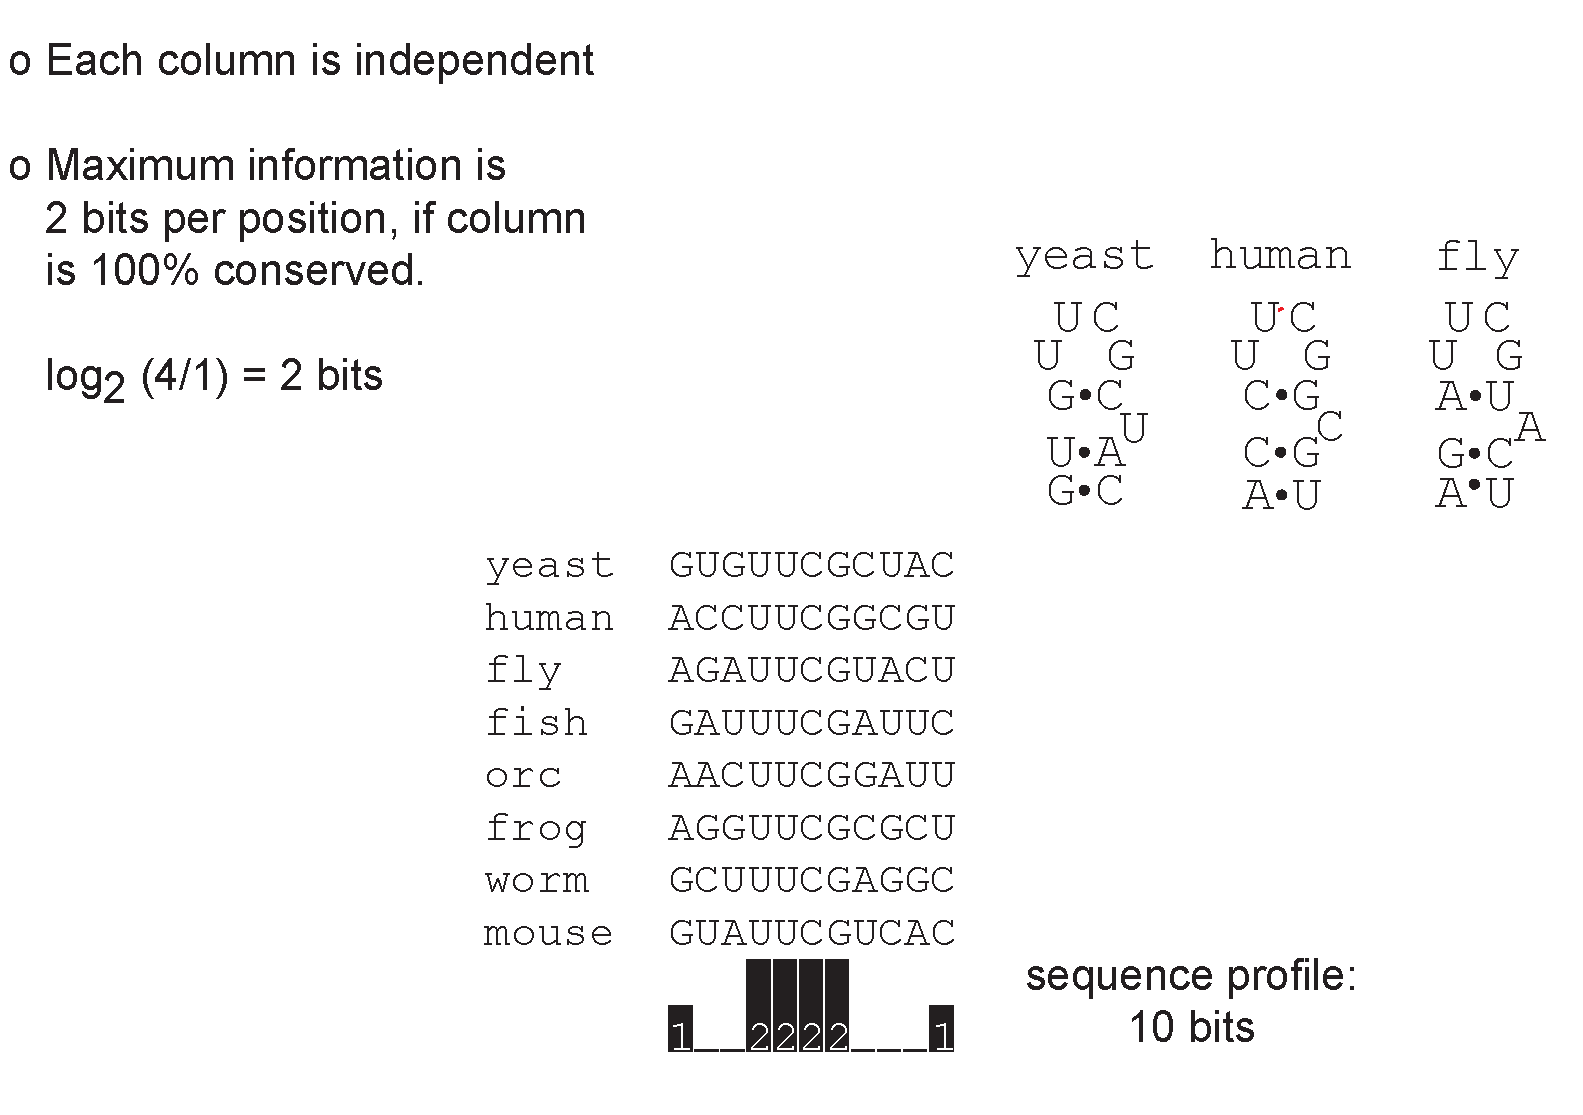
\includegraphics[width=10.5in]{figs/info_for_alignment_primary}
\end{center}

\end{slide}

%%%%%%%%%%%%%%%%%%%%%%%%%%%%%%%%%%%%%%%%%%%%%%%%%%%%%%%%%%%%%%%%%%%%%%
\begin{slide}
\begin{center}
\textbf{RNA sequence analysis with sequence and structure profiles}
\end{center}
\medskip

\begin{center}
%\includegraphics[width=10.5in]{figs/info_structure}
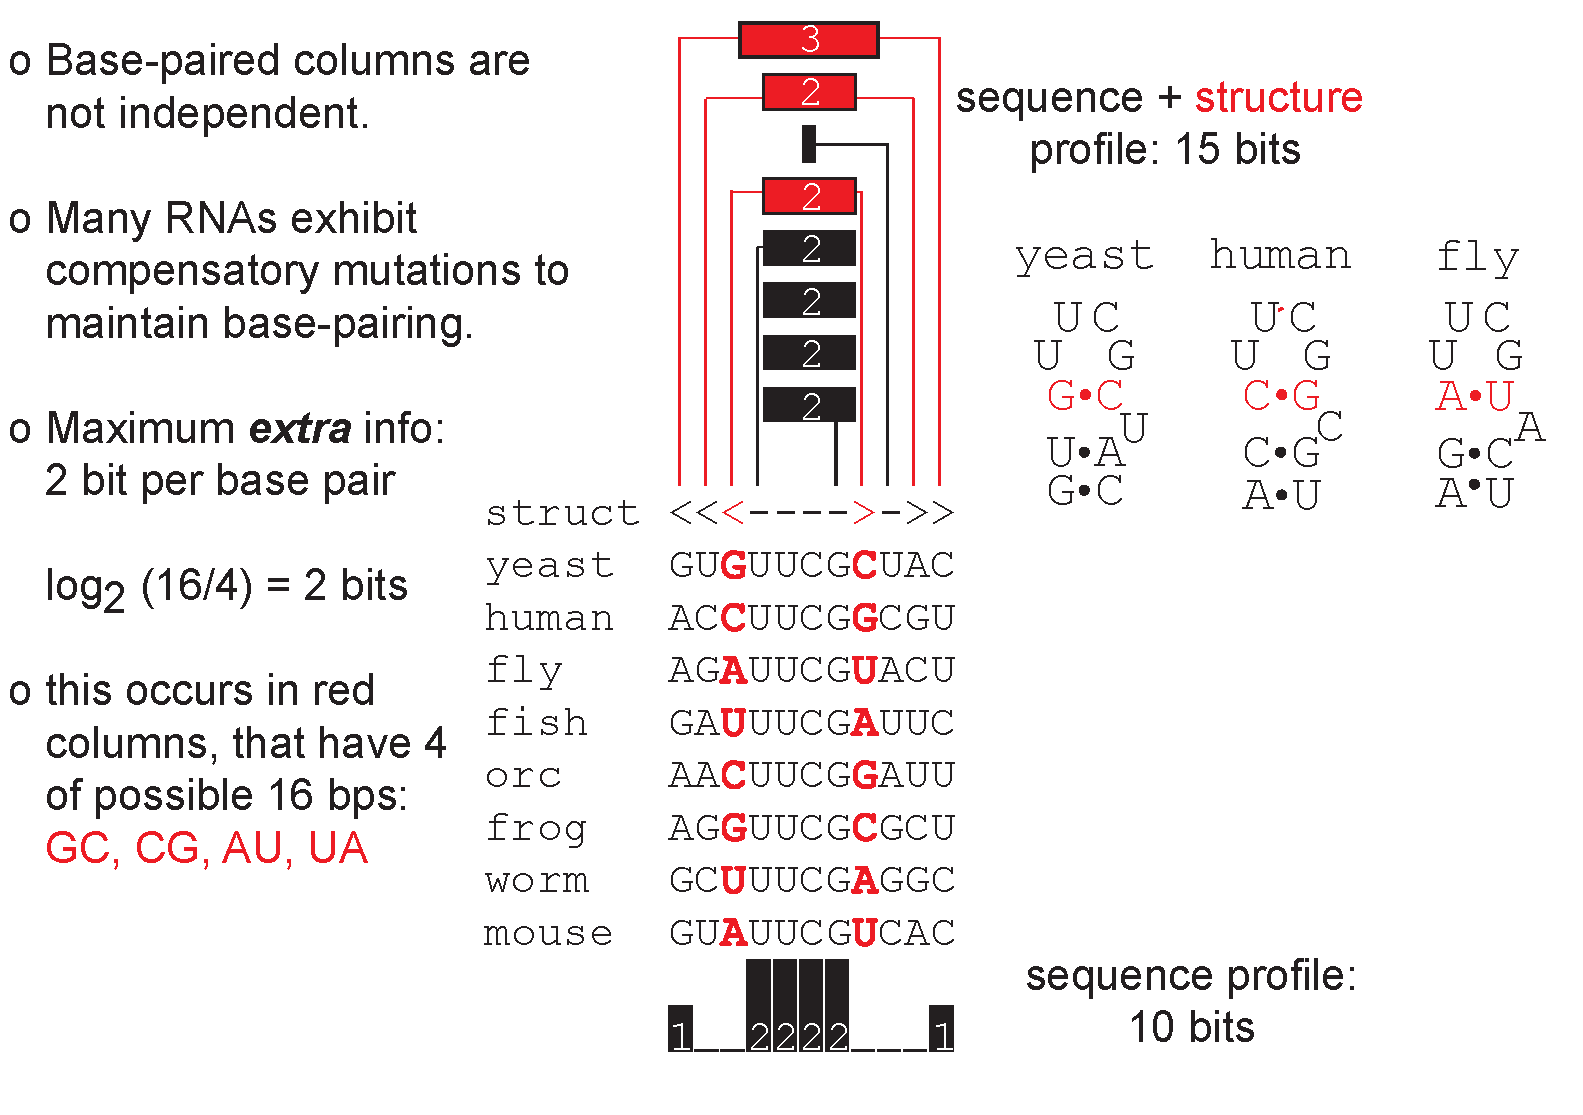
\includegraphics[width=10.5in]{figs/info_for_alignment_structure}
\end{center}

\end{slide}

%%%%%%%%%%%%%%%%%%%%%%%%%%%%%%%%%%%%%%%%%%%%%%%%%%%%%%%%%%%%%%%%%%%%%%%%%%
\begin{slide}
\begin{center}
\textbf{Levels of sequence and structure conservation in RNA families}
\end{center}
\medskip

\begin{center}
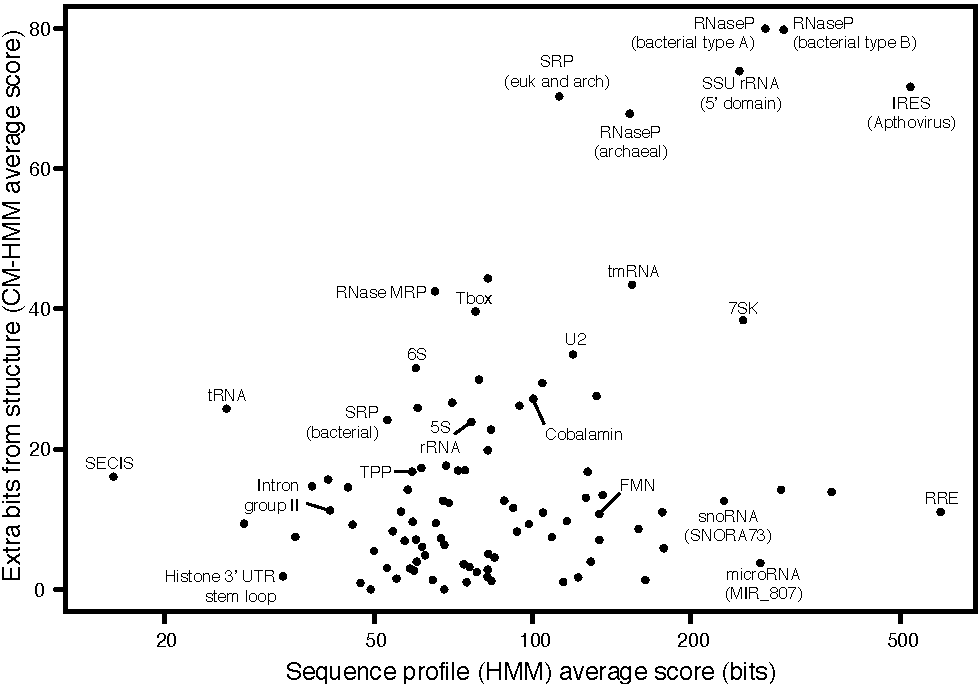
\includegraphics[height=6.5in]{figs/avgscores}
\end{center}

\vfill

\end{slide}
%%%%%%%%%%%%%%%%%%%%%%%%%%%%%%%%%%%%%%%%%%%%%%%%%%%%%%%%%%%%%%%%%%%
\begin{slide}
\begin{center}
%\textbf{profile HMMs and covariance models}
\textbf{Profile probabilistic models}
\end{center}
\medskip

\begin{center}
\small
\begin{tabular}{r|cc} 
             &         & sequence \\
             & sequence& and structure \\
             & profiles& profiles \\ \hline
  \\
  models     & profile HMMs    & profile SCFGs (CMs) \\ 
  \\
  software   & {\sc HMMER}     & {\sc Infernal} \\ 
  \\
  main use   & proteins        & RNAs \\ 
  \\
  database   & {\sc Pfam}      & {\sc Rfam} \\
             & (9318 families) & (1371 families) \\
  \\
%  primary sequence & yes & yes \\
%  \\
%  secondary structure & no & yes \\
%  \\
  algorithms & Viterbi & CYK \\
             & Forward & Inside \\
             &         & \\
  complexity & $O(LN)$ & $O(LN^{2} log N)$ \\
  \\
  performance& faster but    & slower but    \\
  for RNAs   & less accurate & more accurate \\
\end{tabular}

\hspace{1.2in}
\includegraphics[height=1.5in]{figs/hmmer_logo}\hspace{1.05in}
\includegraphics[height=1.8in]{figs/infernal_logo}

\end{center}

\vfill

\end{slide}
%%%%%%%%%%%%%%%%%%%%%%%%%%%%%%%%%%%%%%%%%%%%%%%%%%%%%%%%%%%%%%
\begin{slide}
\begin{center}
\textbf{CMs are much slower than HMMs}
\end{center}
\medskip

% CM search times taken from QDB paper (infernal version 0.72)
% (RF00114 S15 time used instead of 5S, very similar clen and same #bifs)
% all other times calced with infernal 1.0 (see ~/notebook/9_0520_talk_copenhagen/timings/).
% empirically, it seems to get non-banded CYK 1.0 times, multiply the
% 0.72 times by 3 (this speedup was due to a reimplementation of the
% scanning CYK program.
% HMM search: viterbi
% CM search: qdb paper (non-banded CYK)
% HMM align: viterbi
% CM align: cyk D&C no bands
\begin{center}
\small
\begin{tabular}{lr|rr|rr}
                  &        & \multicolumn{2}{c|}{search (min/Mb)} &   \multicolumn{2}{c}{alignment (sec/seq)}\\ \cline{3-6}
                  &        &        &        &         &  \\
family            & length & HMM    & CM     &    HMM  & CM  \\ \hline
                  &        &        &        &         &  \\
%tRNA              & 71     &  0.06m &  40.5 &  0.0002&   0.05  \\
tRNA              & 71     &  0.17 &  13.5 &  0.0002&   0.05  \\
                  &        &        &        &         &  \\
5S rRNA           & 119    &  0.27 &  17.8 &  0.0005&   0.2  \\
                  &        &        &        &        &  \\
Lysine riboswitch & 183    &  0.40  & 57.1 &  0.001 &   0.8 \\
                  &        &        &        &         &  \\
SRP RNA           & 304    &  0.66  & 147.8 &  0.003 &   5.4 \\
                  &        &        &        &         &  \\
RNaseP            & 365    &  0.78 & 334.4 &  0.005 &  12.0 \\
                  &        &        &        &         &  \\
%SSU rRNA          & 1466   &  0.93 &    -   &  0.08  & 795.6 \\
SSU rRNA          & 1466   &  4.00 & 7660.0&  0.08  & 795.6 \\
                  &        &        &        &         &  \\
\end{tabular}
\end{center}

\vfill

\end{slide}
%%%%%%%%%%%%%%%%%%%%%%%%%%%%%%%%%%%%%%%%%%%%%%%%%%%%%%%%%%%%%%%%%%

\begin{slide}
\begin{center}
\large
\textbf{Small subunit ribosomal RNA and the tree of life}
\end{center}
\medskip
\begin{minipage}{5.2in}
\small

\begin{itemize}
\item
1977 - Carl Woese decided to classify all living things phylogenetically
\item
needed ``\emph{a molecule of appropriately broad distribution}'' for
comparative analysis
\item
SSU rRNA was chosen
\begin{itemize}
  \item
    universally distributed
  \item
    highly constrained throughout \\ evolution
  \item
    large enough to provide sufficient data% (1500-1800 nt)
  \item
    readily isolated
\end{itemize}
\end{itemize}

\vspace{2.5in}
\end{minipage}
\hspace{0.1in}
\begin{minipage}{5.5in}
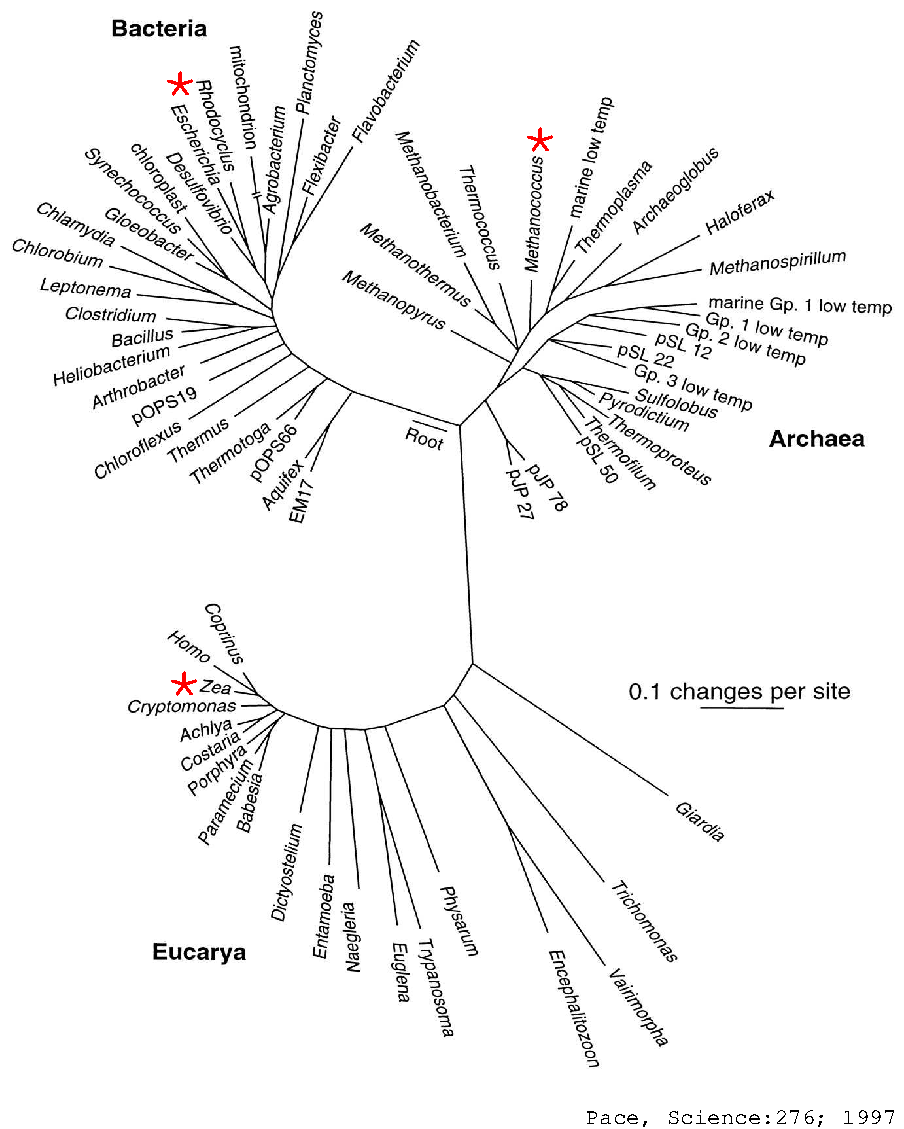
\includegraphics[width=5.5in]{figs/bigtol}
%\vspace{1.5in}
\end{minipage}  

\end{slide}

%%%%%%%%%%%%%%%%%%%%%%%%%%%%%%%%%%%%%%%%%%%%%%%%%%%%%%%%%%%%%%%%%%%%%%%%%%
%Slide 2 - SSU rRNA is very well conserved across all three domains
\begin{slide}
\begin{center}
\large
\textbf{Universal structural conservation of SSU rRNA}
\end{center}
\vspace{0.5in}
\small
\hspace{0.75in}
\emph{Escherichia coli}
\hspace{1.2in}
\emph{Methanococcus vannielii}
\hspace{1.2in}
\emph{Zea mays}

\begin{center}
%\includegraphics[height=4.6in]{figs/ecoli_16S}
%\includegraphics[height=4.6in]{figs/mvan_16S}
%\includegraphics[height=4.6in]{figs/zmays_16S}
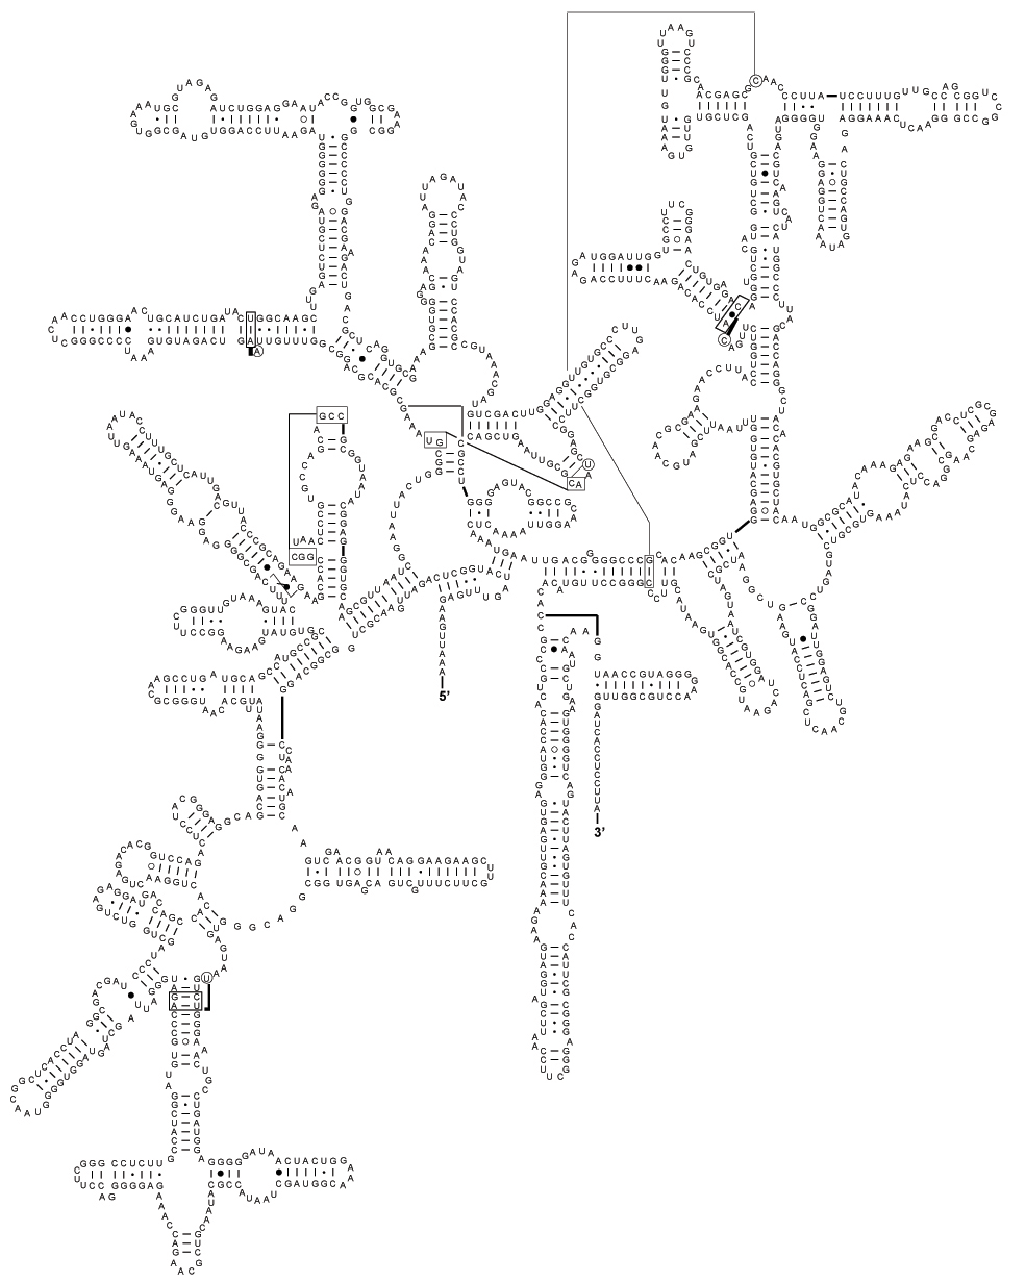
\includegraphics[height=4.45in]{figs/ecoli_16S_man}
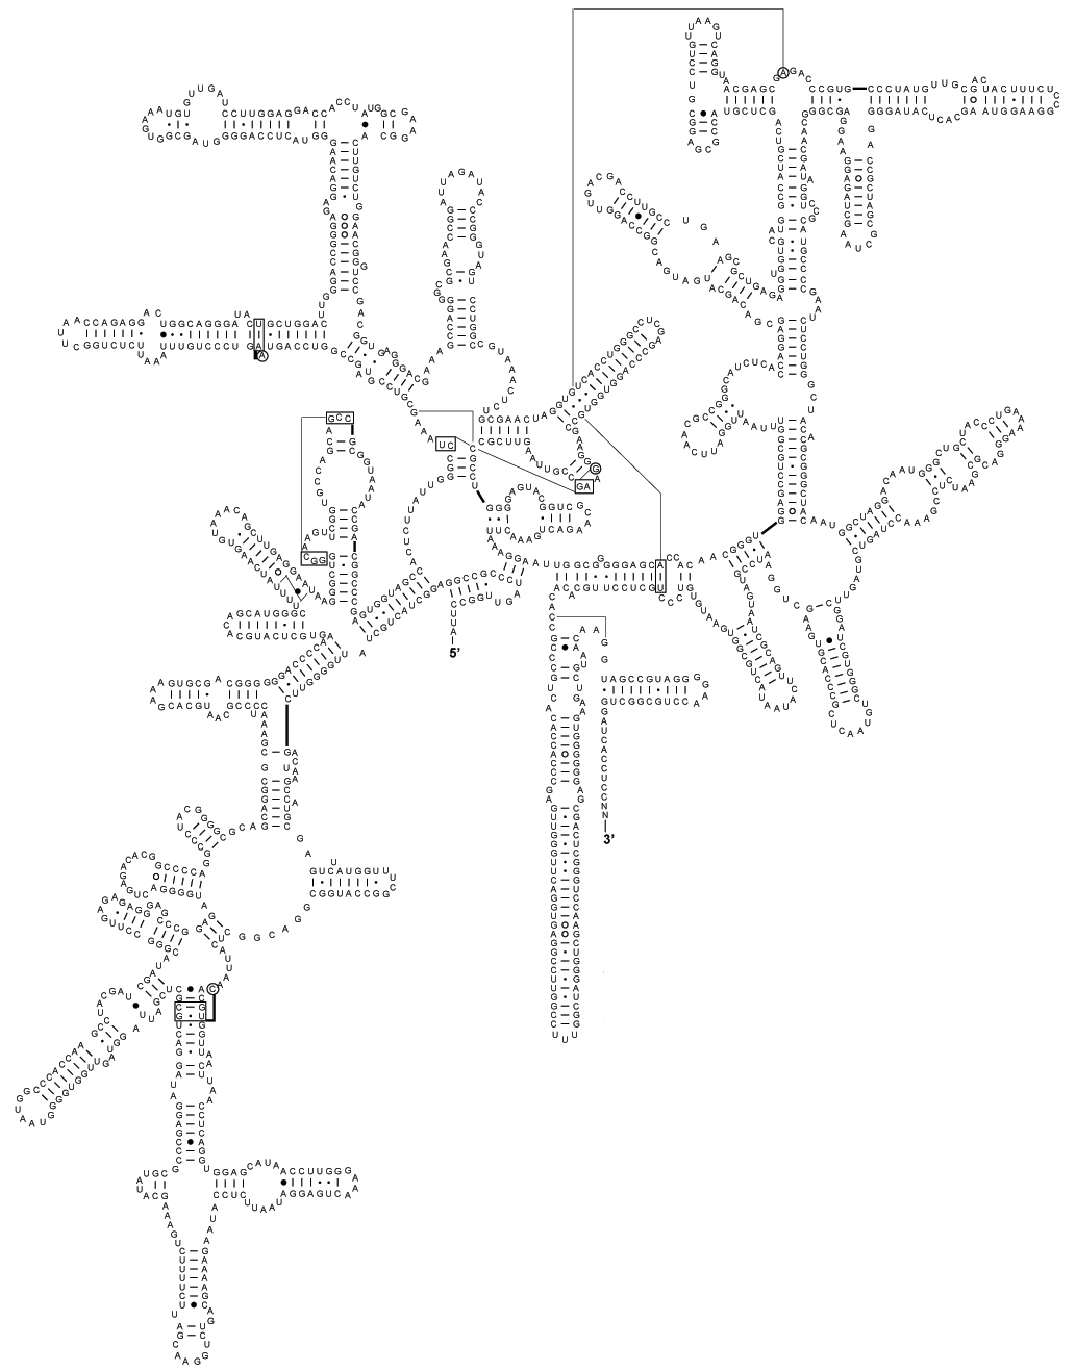
\includegraphics[height=4.45in]{figs/mvan_16S_man}
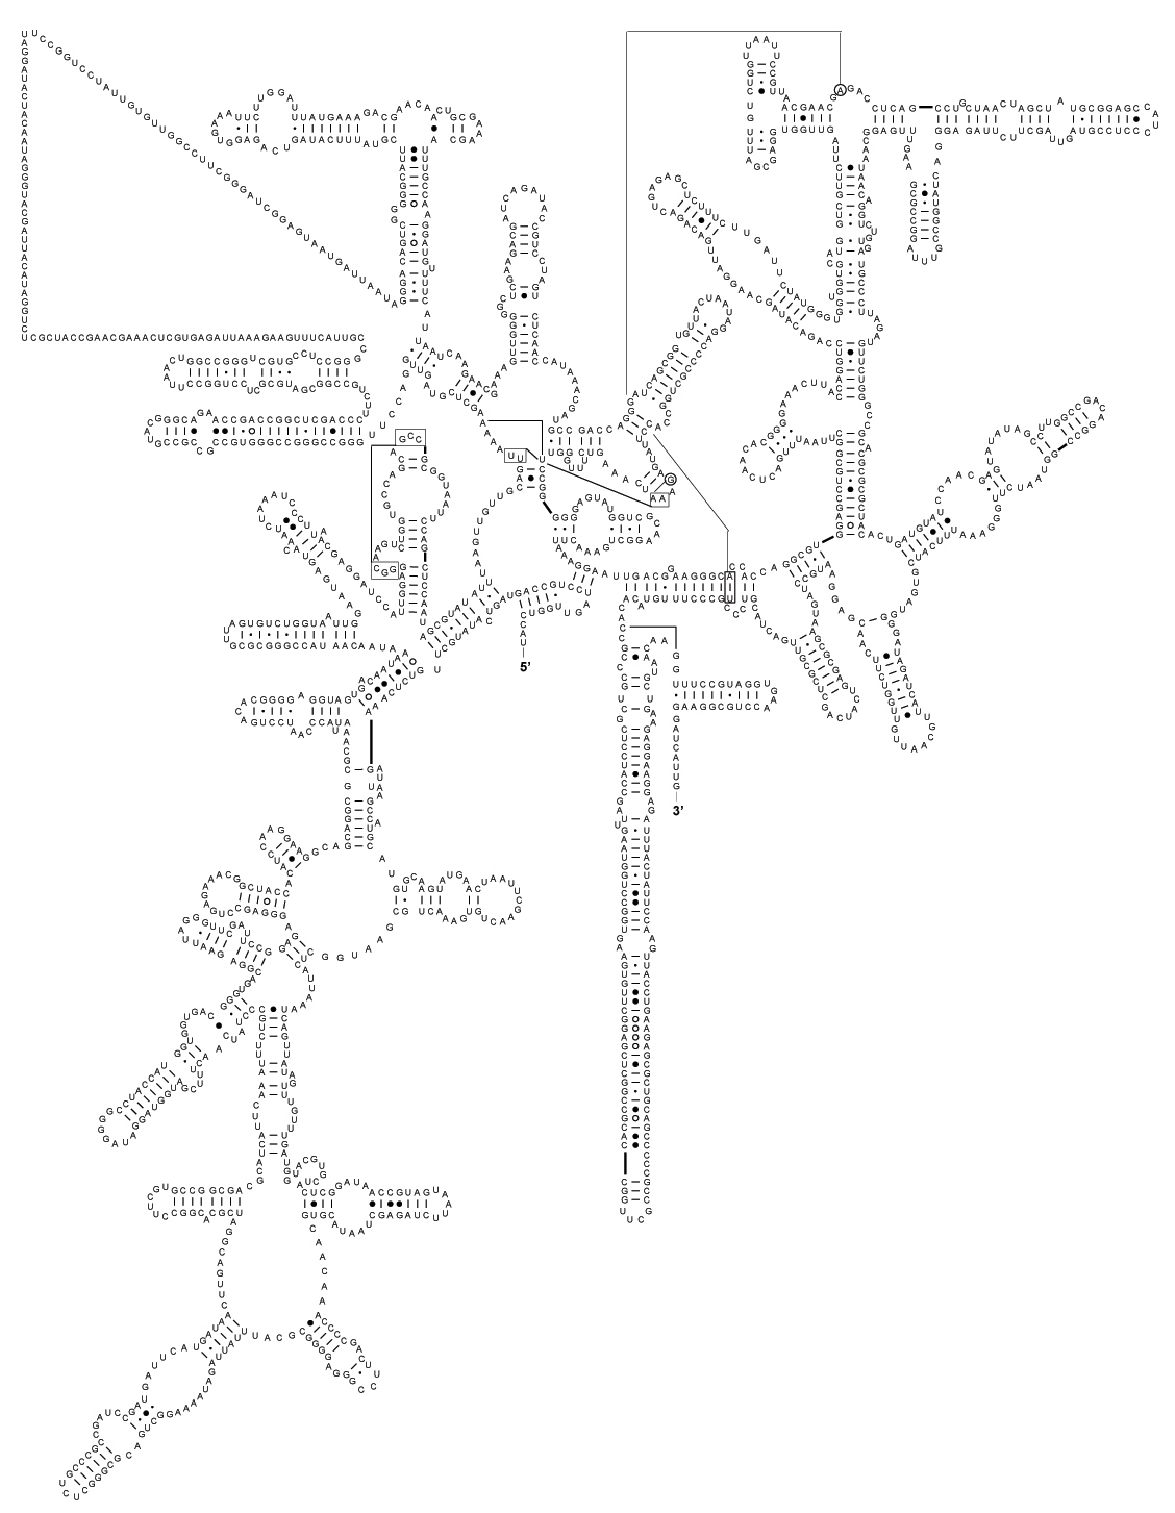
\includegraphics[height=4.45in]{figs/zmays_16S_man}
\end{center}

\begin{flushright}
\tiny{\texttt{Secondary structure diagrams from:}} \\
\tiny{\texttt{URL:http://www.rna.icmb.utexas.edu/}}
\end{flushright}
%should this slide have a tree of life? if not where should it go?
\vfill
\end{slide}

%%%%%%%%%%%%%%%%%%%%%%%%%%%%%%%%%%%%%%%%%%%%%%%%%%%%%%%%%%%%%%%%%%%%%%%%%%
%Slide 2 - SSU rRNA is very well conserved across all three domains
\begin{slide}
\begin{center}
\large
%\textbf{Universal sequence conservation of SSU rRNA}
\textbf{Sequence conservation in SSU rRNA}
\end{center}
\vspace{0.5in}
\small
\hspace{1.5in}
\underline{bacteria}
\hspace{2.2in}
\underline{archaea}
\hspace{2.2in}
\underline{eukarya}

\begin{center}
%\includegraphics[height=4.6in]{figs/ecoli_16S}
%\includegraphics[height=4.6in]{figs/mvan_16S}
%\includegraphics[height=4.6in]{figs/zmays_16S}
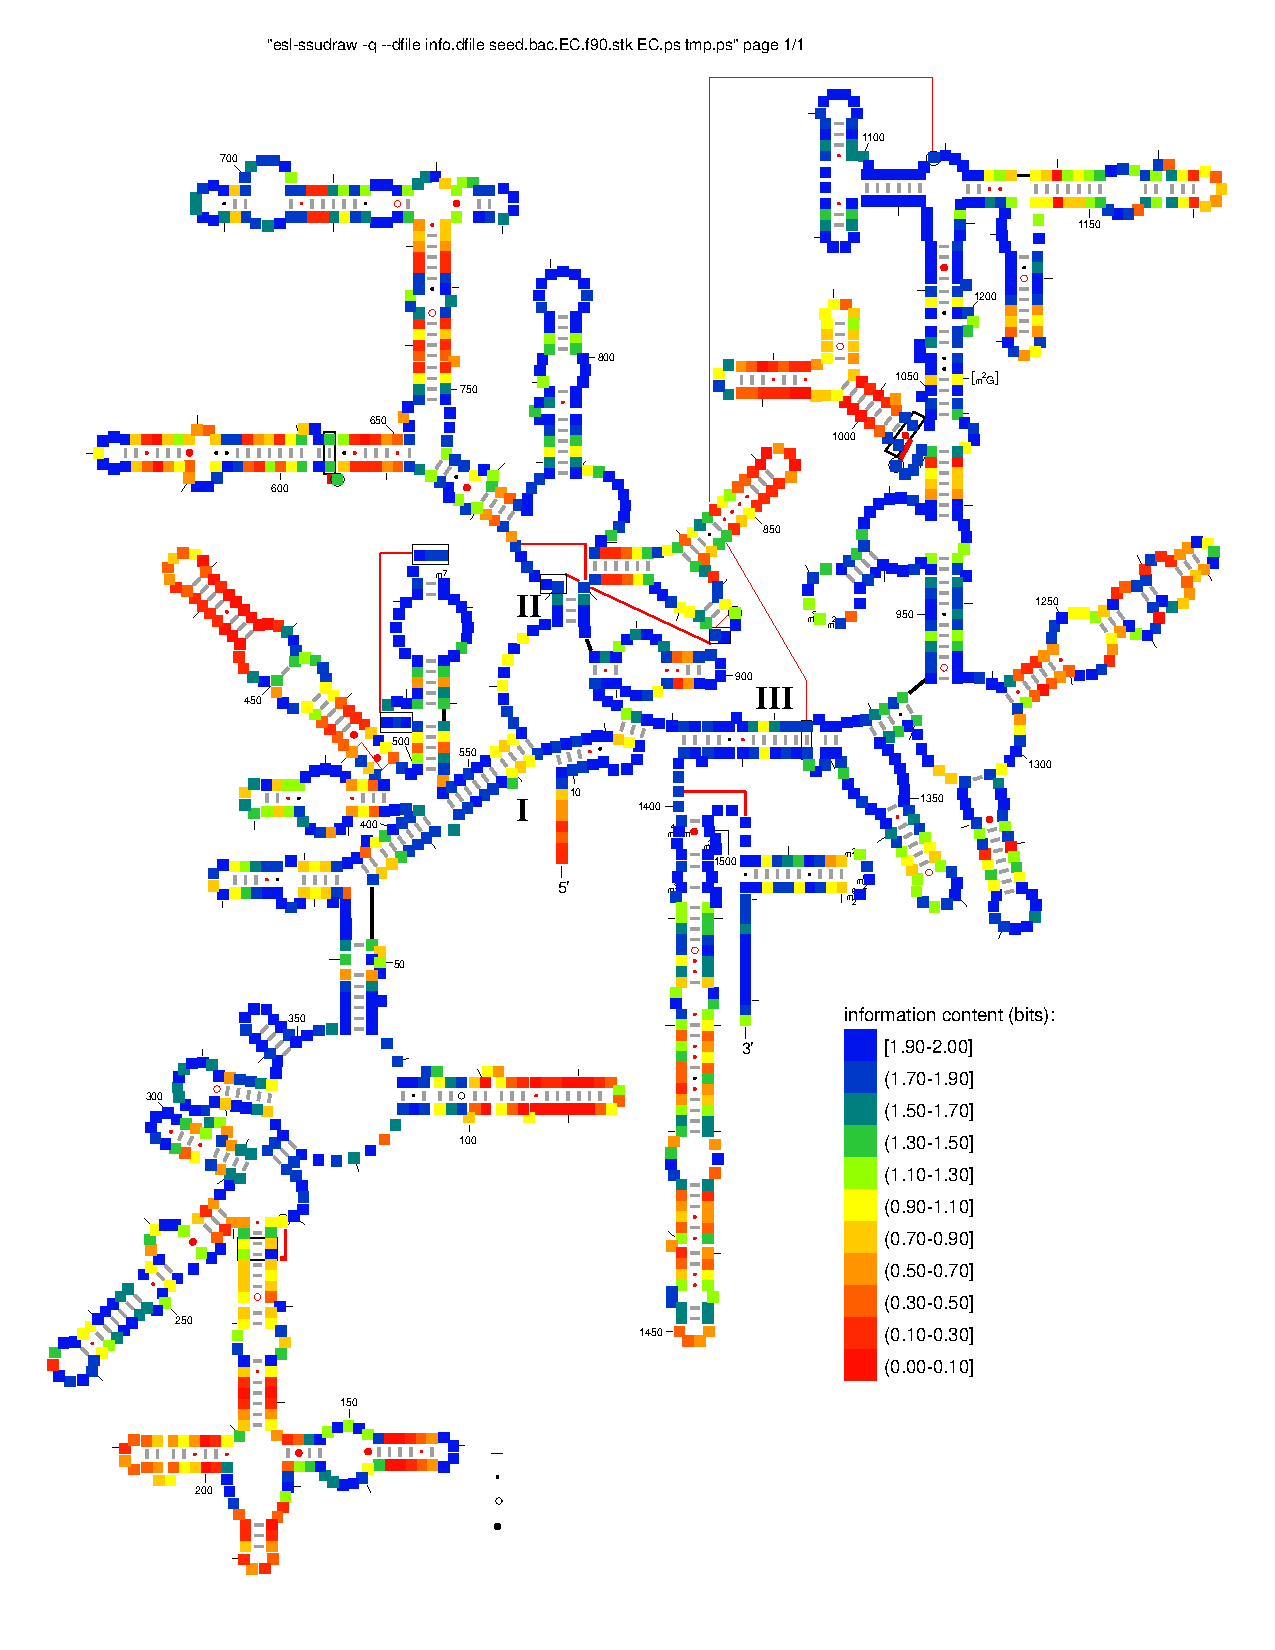
\includegraphics[height=4.45in]{figs/bac_info_heat}
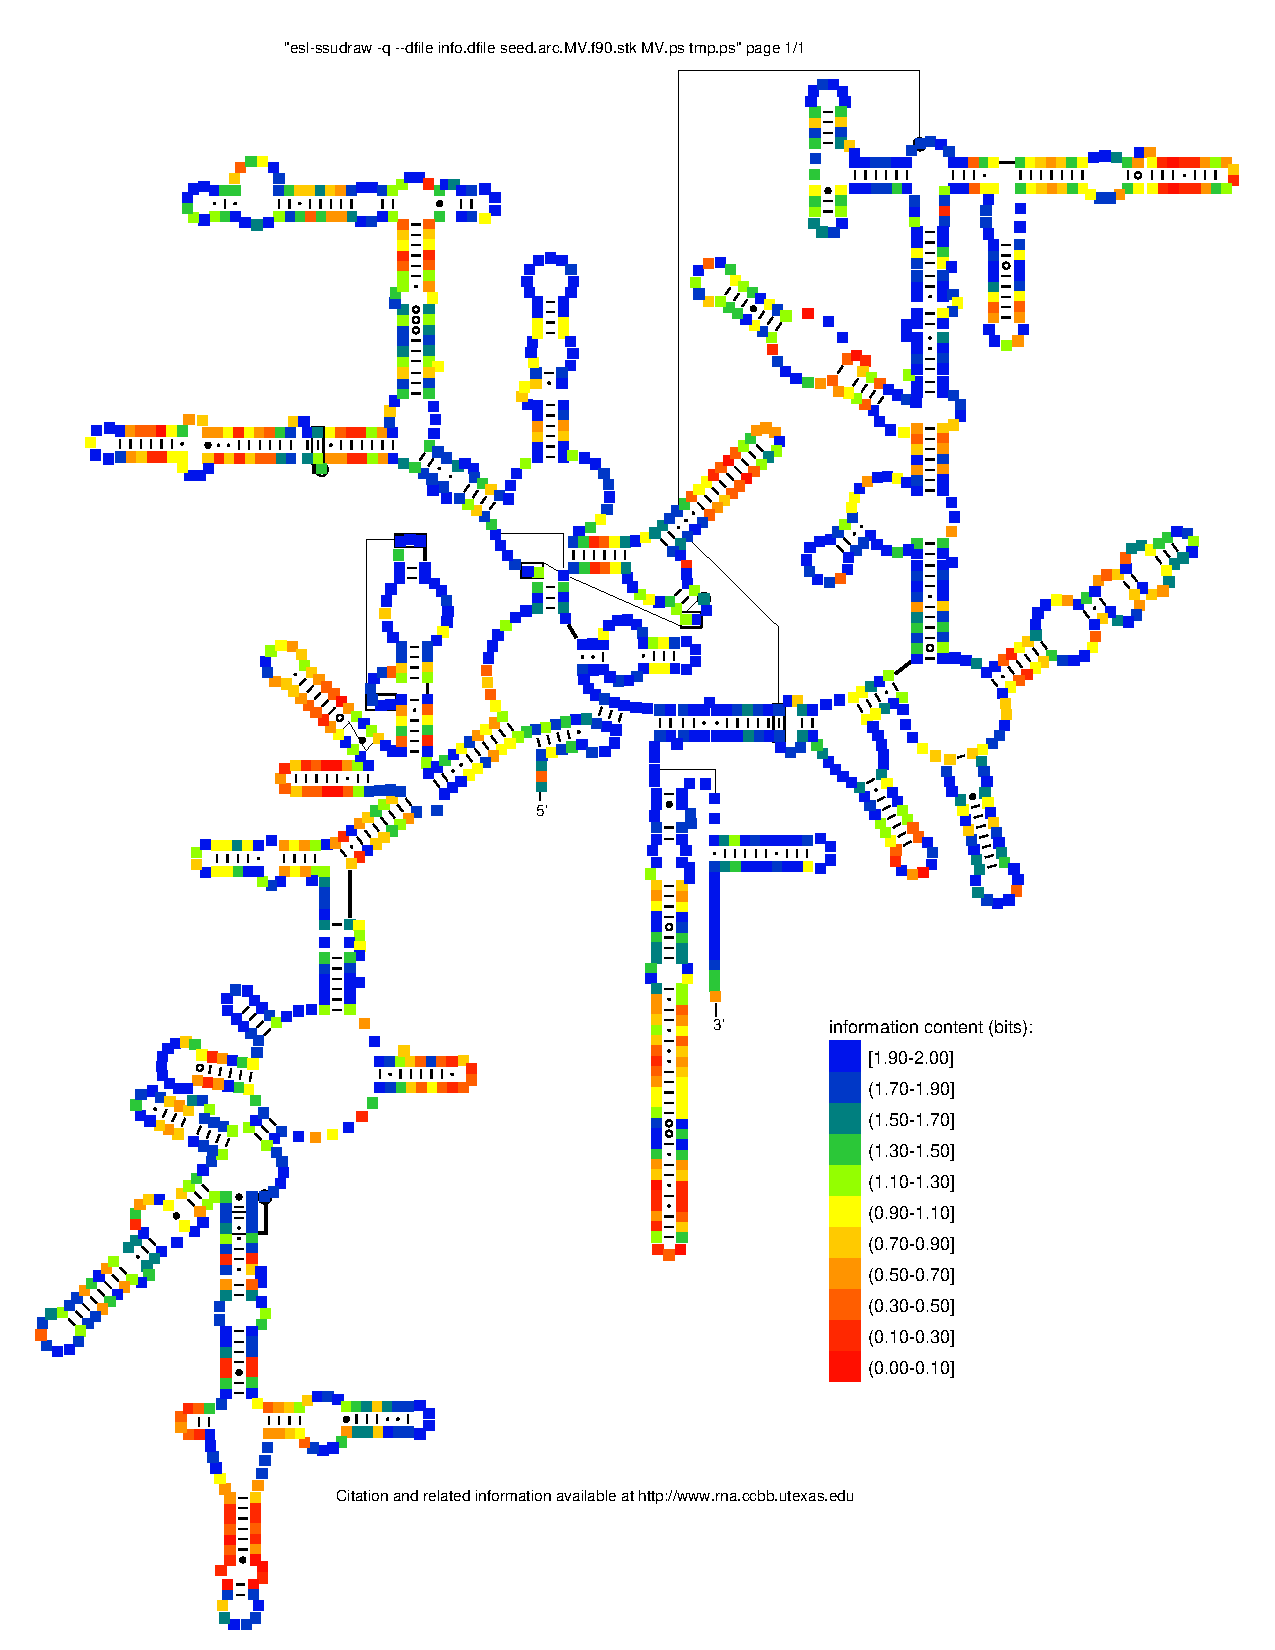
\includegraphics[height=4.45in]{figs/arc_info_heat}
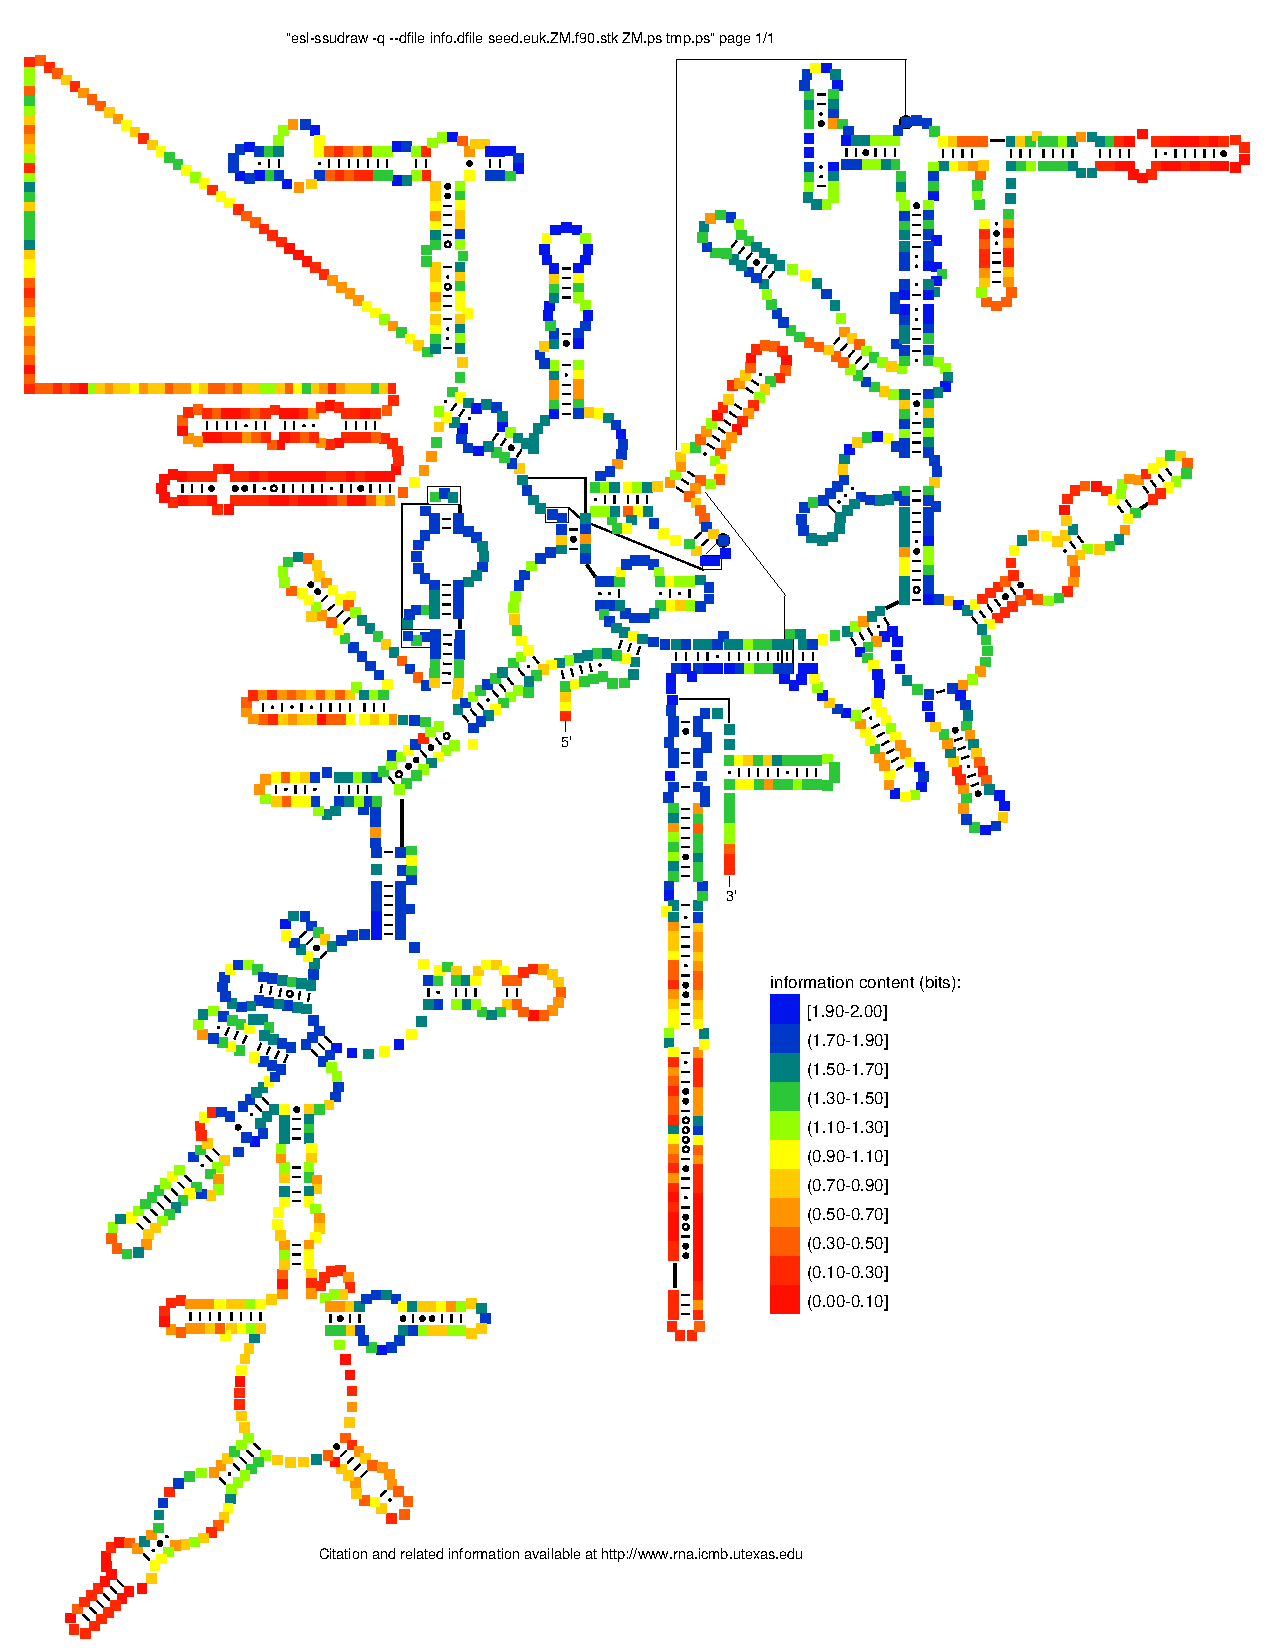
\includegraphics[height=4.45in]{figs/euk_info_heat}
\end{center}

\begin{flushright}
\tiny{\texttt{Secondary structure diagrams created based}} \\
\tiny{\texttt{alignments and diagrams from:}} \\
\tiny{\texttt{URL:http://www.rna.icmb.utexas.edu/}}
\end{flushright}
\vfill
\end{slide}

%%%%%%%%%%%%%%%%%%%%%%%%%%%%%%%%%%%%%%%%%%%%%%%%%%%%%%%%%%%%%%%%%%%%%%%%%%
%%%%%%%%%%%%%%%%%%%%%%%%%%%%%%%%%%%%%%%%%%%%%%%%%%%%%%%%%%%%%%%%%%%%%%%%%%
% Slide 3 Environmental sequencing surveys target SSU rRNA
% 
% Introduce how environmental sequencing surveys require alignment to 
% to phylogenetic inference
% To do : add more specifics on environmental sequencing studies?
%       : shotgun sequencing? universal primers?


\begin{slide}
\begin{center}
\large
\textbf{Environmental surveys target SSU}
\end{center}
\medskip
\begin{minipage}{7in}
\small
\begin{itemize}
\item
mid 1980s - Norman Pace develops methodology for determination of SSU
sequences without cultivation
% for determining SSU sequences
%from microorganisms without cultivation
\item
%``the great plate-count anomaly'' - microorganisms that can grow in a
%  laboratory constitute less than 1\% of all microbial species
``the great plate-count anomaly'' - vast \\ majority of microbial species
  cannot be cultivated
\item
environmental surveys have become common
\begin{itemize}
  \item
    many different environments have been studied
  \item
    commonly expand known biodiversity
    \begin{itemize}
      \item
	recognized bacterial phyla: \\
	11 in 1987, 36 in 1998, 52 in 2003, 67 in 2006...
    \end{itemize}
\end{itemize}
\end{itemize}
\center{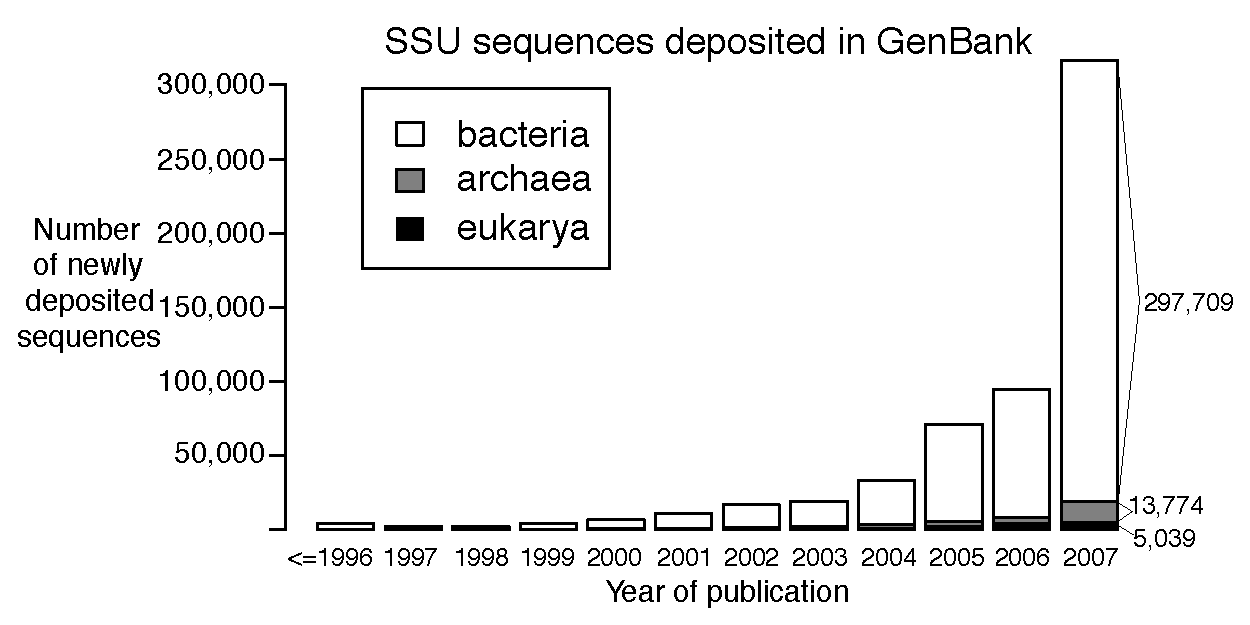
\includegraphics[height=3.3in]{figs/ncbi-ssu-gb}}

\vspace{.7in}
\end{minipage}
\hspace{0.1in}
\begin{minipage}{3in}
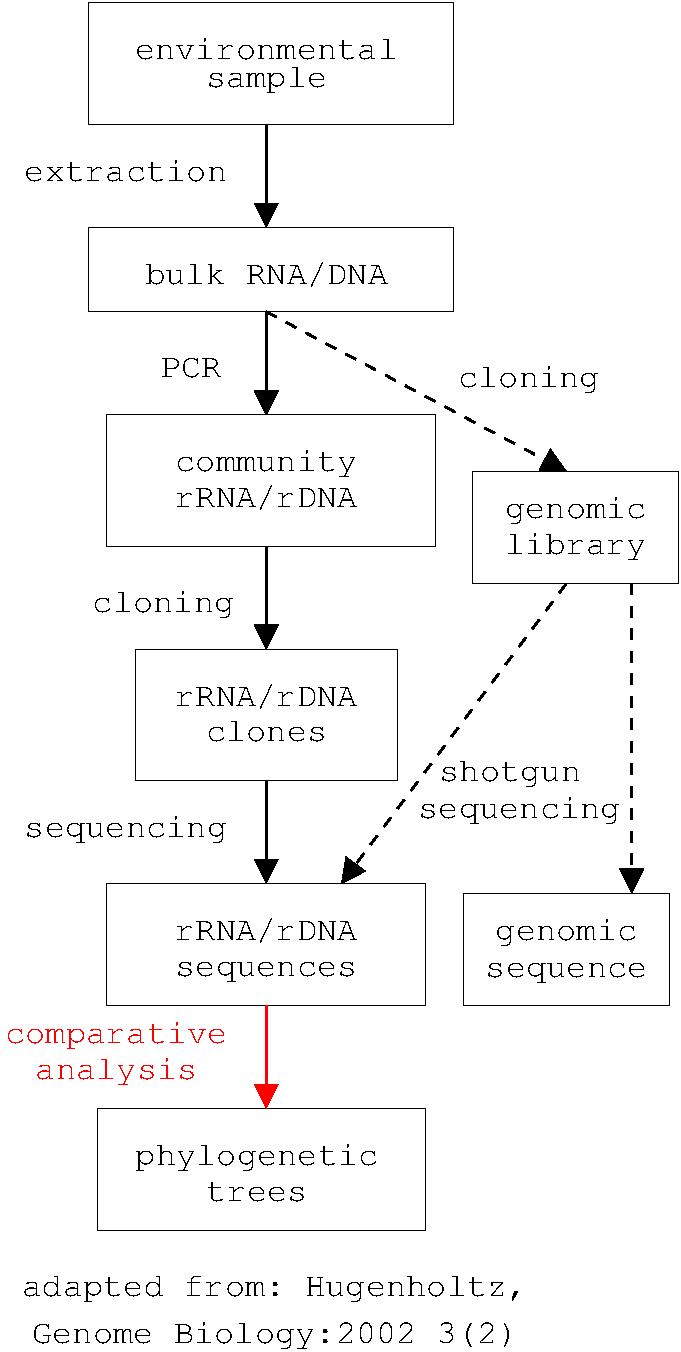
\includegraphics[height=6in]{figs/environmental}
\vspace{1in}
\end{minipage}
\end{slide}

%%%%%%%%%%%%%%%%%%%%%%%%%%%%%%%%%%%%%%%%%%%%%%%%%%%%%%%%%%%%%%%%%%%%%%%%%%
\begin{slide}
\begin{center}
\large
\textbf{Environmental surveys target SSU rRNA}
\end{center}

%\includegraphics[height=6in]{figs/ssu_gb_surveys_list_2007}
\center{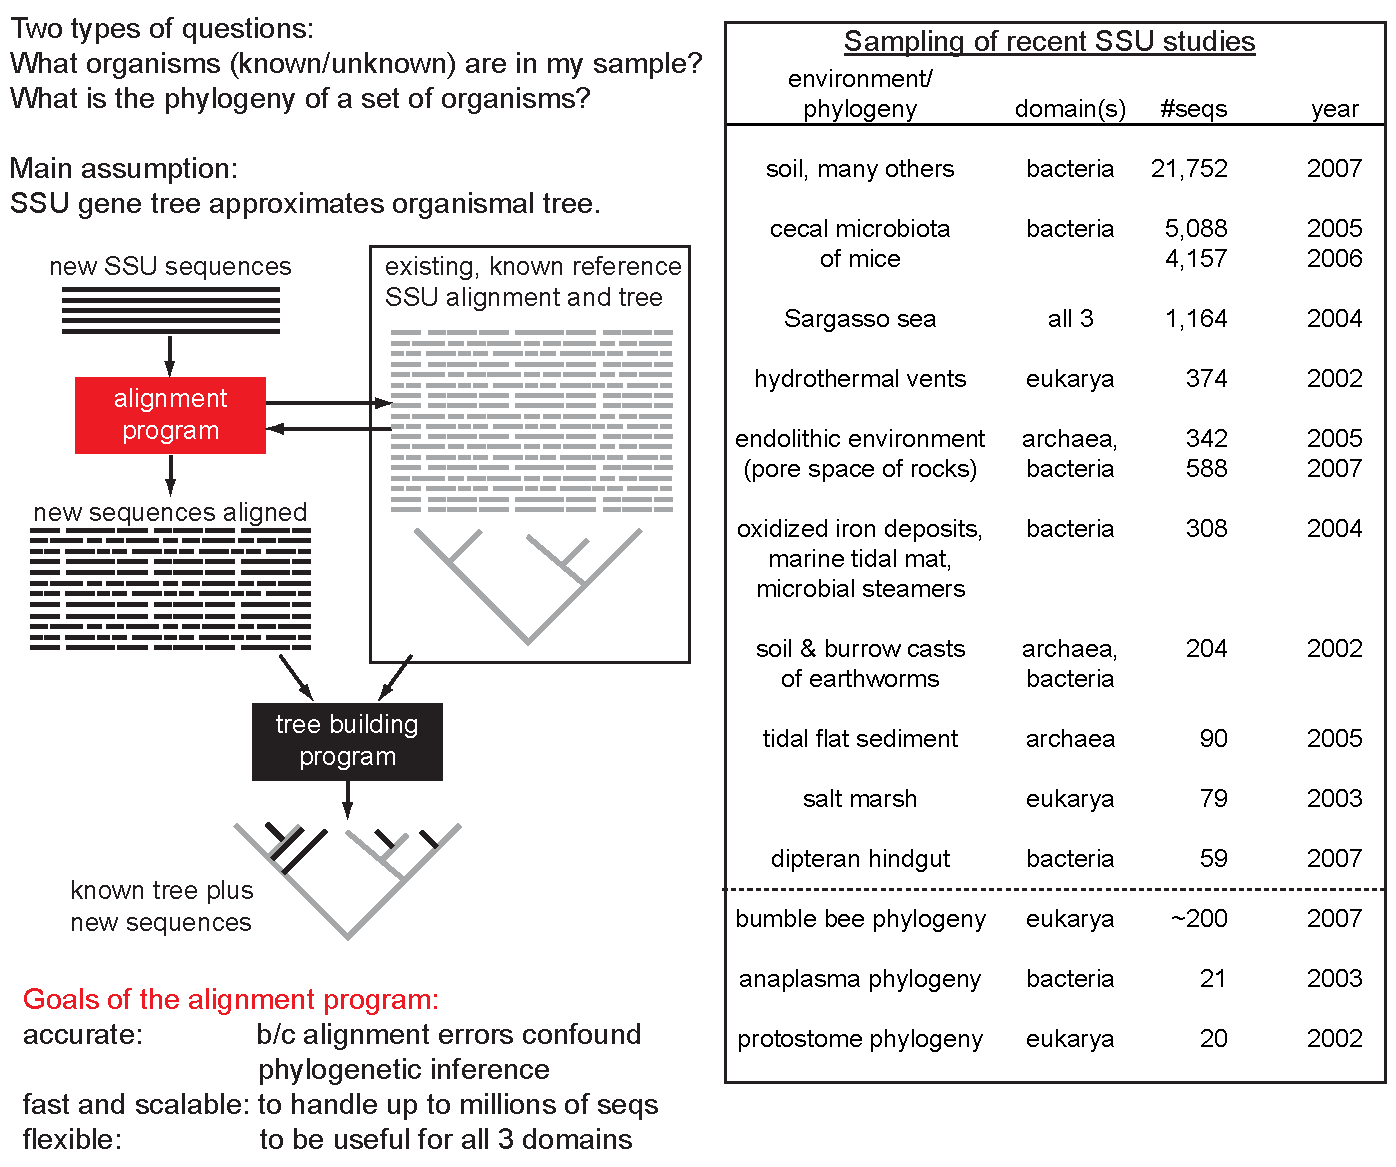
\includegraphics[height=7in]{figs/ssu_list_and_seq2tree_blackgrey}}
%\center{\includegraphics[height=7in]{figs/ssu_list_and_seq2tree_bluegold}}
\vfill
\end{slide}
%%%%%%%%%%%%%%%%%%%%%%%%%%%%%%%%%%%%%%%%%%%%%%%%%%%%%%%%%%%%%%%%%%%%%%%%%%
\begin{slide}
\begin{center}
\large
\textbf{Environmental surveys target SSU rRNA}
\end{center}
%\includegraphics[height=6in]{figs/ssu_gb_surveys_list_2007}
\center{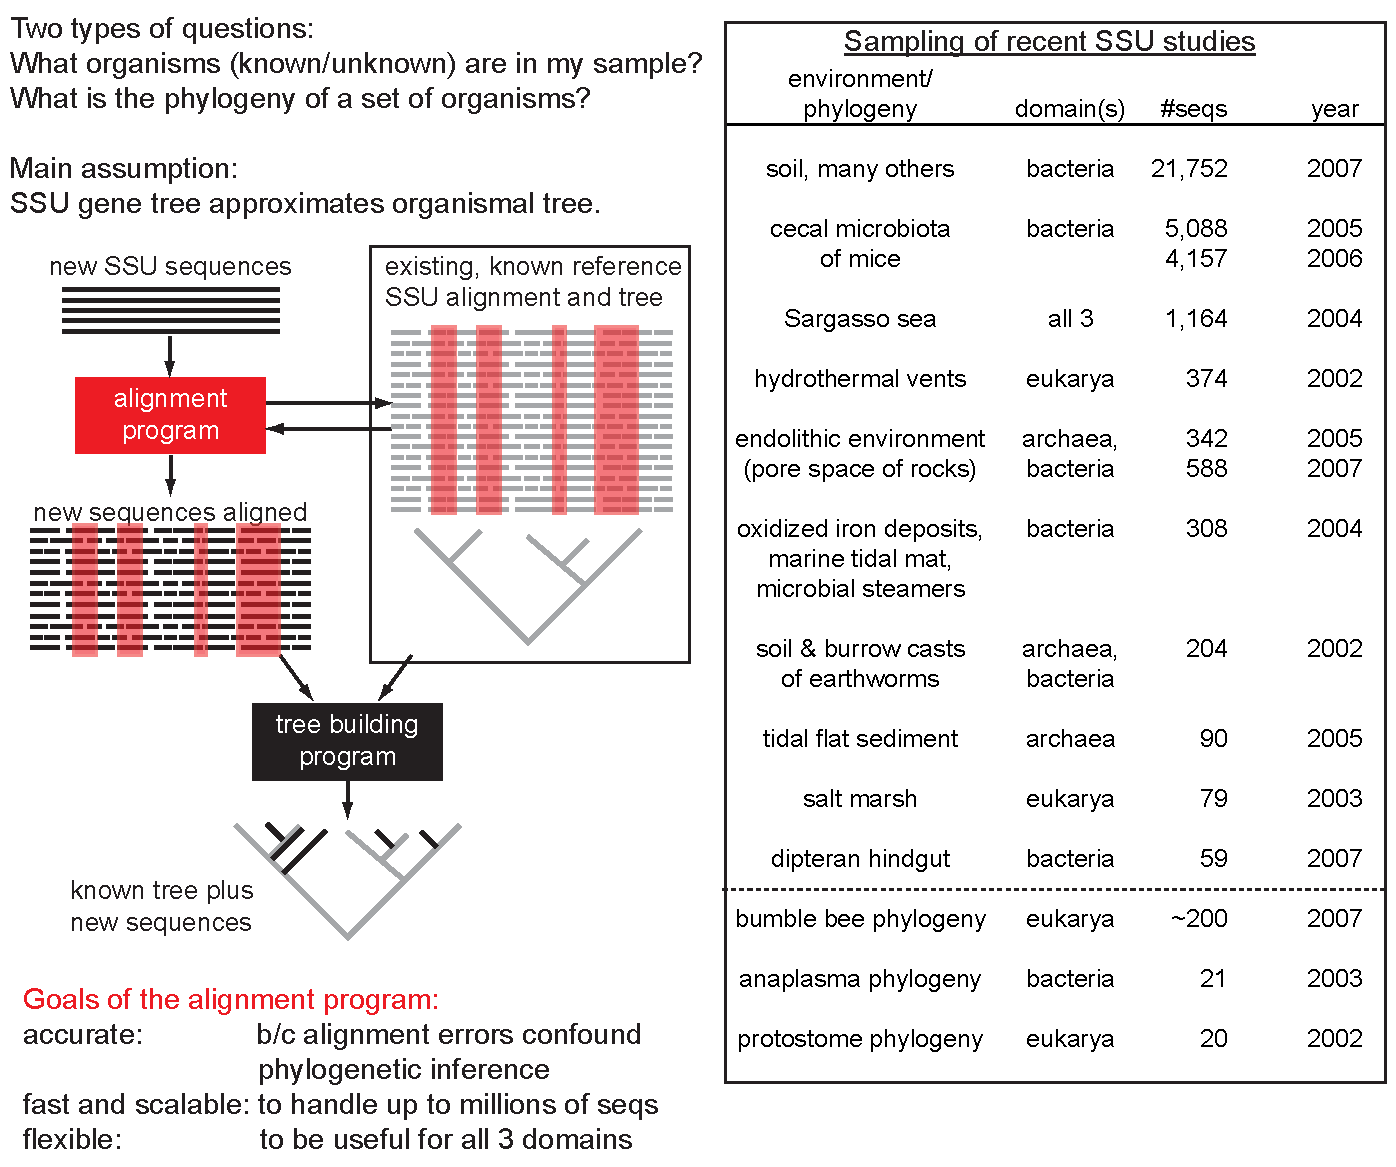
\includegraphics[height=7in]{figs/ssu_list_and_seq2tree_blackgrey_wredmask}}
%\center{\includegraphics[height=7in]{figs/ssu_list_and_seq2tree_blackgrey_wmask}}
%\center{\includegraphics[height=7in]{figs/ssu_list_and_seq2tree_bluegold}}
\vfill
\end{slide}
%%%%%%%%%%%%%%%%%%%%%%%%%%%%%%%%%%%%%%%%%%%%%%%%%%%%%%%%%%%%%%%%%%%%%%%%%%
\begin{slide}
\begin{center}
%\large
\textbf{profile HMMs and covariance models}: speed versus accuracy
\end{center}
\medskip

%\begin{itemize}
%\item
%  Different RNA families exhibit a range of sequence and structural
%  conservation: 

\begin{minipage}{6in}
\begin{center}
\small
\begin{tabular}{r|cc|} 
             & profile & covariance  \\
             & HMMs    & models (CMs) \\ \hline
  & & \\
  software   & {\sc HMMER}     & {\sc Infernal} \\ 
  & & \\
%  database   & {\sc Pfam}      & {\sc Rfam} \\
%             & (9318 families) & (607 families) \\
%  & & \\
%  primary sequence & yes & yes \\
  primary & yes & yes \\
  sequence & & \\
  & & \\
  secondary & no & yes \\
  structure & & \\
%  secondary structure & no & yes \\
%  \\
%  algorithm  & Viterbi & CYK \\
%             & Forward & Inside \\
  & & \\
  complexity & $O(N^2)$ & $O(N^{3} log N)$ \\
  & & \\
  performance& faster but    & slower but    \\
  for SSU    & less accurate      & more accurate \\
  rRNAs      & (0.08 sec/seq)     & (795 sec/seq) \\
\end{tabular}
\end{center}
\hspace{2.1in}
\includegraphics[height=1.5in]{figs/hmmer_logo}\hspace{0.65in}
\includegraphics[height=1.8in]{figs/infernal_logo}

\normalsize
%\begin{center}
\center{\textbf{Ideally, we'd like the speed of HMMs and the accuracy of CMs}}
%\end{center}
\vspace{0.1in}
\end{minipage}
\hspace{0.5in}
\begin{minipage}{4in}
\begin{center}
%\includegraphics[width=4in]{figs/pm_intro_seeds_BPS_layer2}
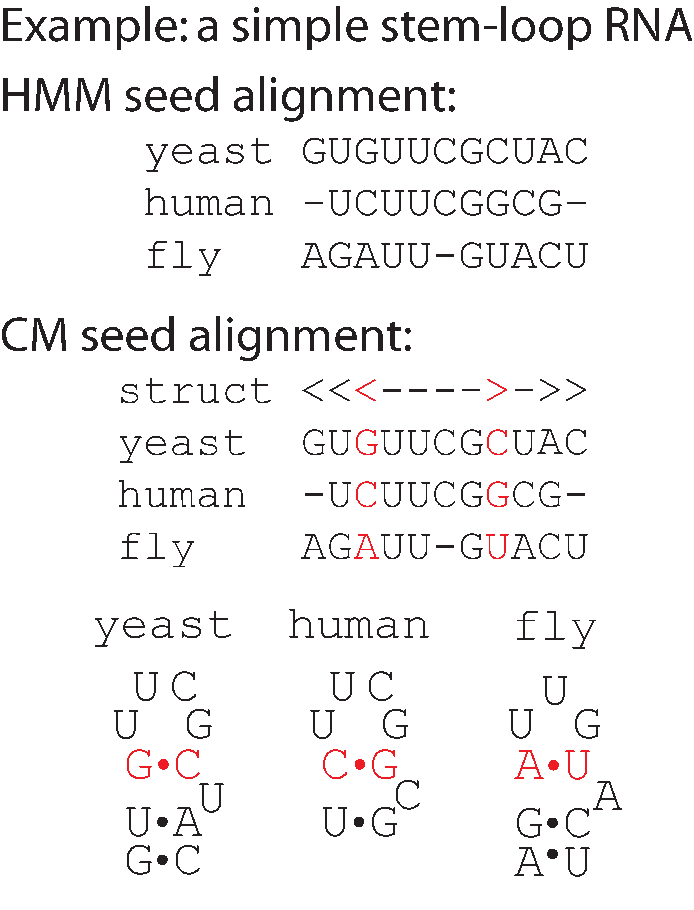
\includegraphics[width=4in]{figs/pm_intro_seeds}
\vspace{1.5in}
\end{center}
\end{minipage}
\vfill

\end{slide}
%%%%%%%%%%%%%%%%%%%%%%%%%%%%%%%%%%%%%%%%%%%%%%%%%%%%%%%%%%%%%%%%%%%%%%%%%%%%%%%%%%%%%%%%%%%%%
%%%%%%%%%%%%%%%%%%%%%%%%%%%%%%%%%%%%%%%%%%%%%%%%%%%%%%%%%%%%%%%%%%%%%%%%%%
\begin{comment}
\begin{slide}
\begin{center}
\large
\textbf{Alignment using profiles}
\end{center}
\medskip
\small
\begin{itemize}
\item
\textbf{main idea:} use fast HMM when it's accurate, appealing to CM when it's not
\item
need some type of measure of confidence in regions of the HMM alignment
\item
requires some type of a \emph{map} from HMM to CM
\end{itemize}
\vfill
\end{slide}
\end{comment}
%%%%%%%%%%%%%%%%%%%%%%%%%%%%%%%%%%%%%%%%%%%%%%%%%%%%%%%%%%%%%%%%%%%%%%%%%%
\begin{slide}
\begin{center}
\large
\textbf{Accelerating CM alignment using HMMs}
\end{center}
\medskip
\begin{minipage}{6in}
\footnotesize
\begin{itemize}
\item
\textbf{main idea:} use fast HMM when it's accurate, appealing to CM when it's not
\item
%requires a method for determining the level of confidence
%(probability) that regions of the HMM alignment are correct 
%need to know the confidence level that regions of the HMM alignment
%are correct
need some type of measure of confidence in regions of the HMM alignment

\end{itemize}
\small
\hspace{0.3in}
\underline{HMM alignment}%\hspace{1.5in}---- $>$
\begin{itemize}
%\item
%each column of 2D dynamic programming \\ matrix corresponds to a column
%of the seed alignment
%\item
%each row of the matrix corresponds to a \\ position of the new sequence
\item
each column of the grid corresponds to a \\ column
of the seed alignment
\item
each row of the grid corresponds to a \\ position of the new sequence
\end{itemize}
\vspace{3in}
\end{minipage}
\begin{minipage}{4in}
\begin{center}
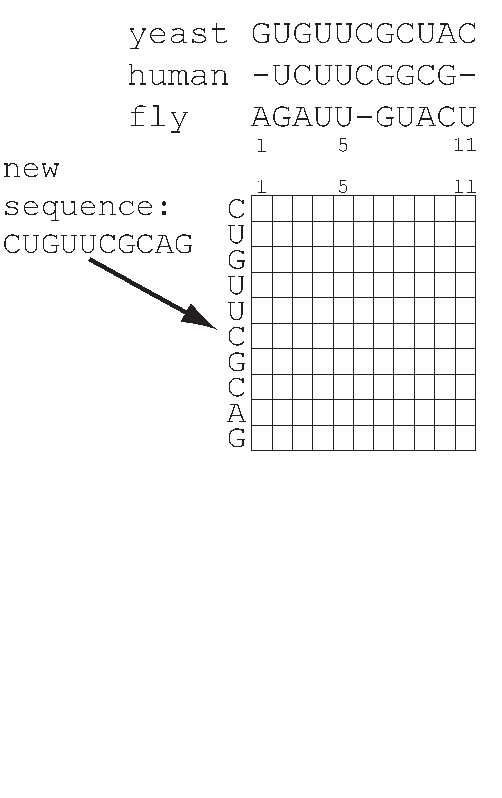
\includegraphics[height=6in]{figs/hmm_alignment2_layer1}
\end{center}
\vspace{1.5in}
\end{minipage}
\end{slide}
%%%%%%%%%%%%%%%%%%%%%%%%%%%%%%%%%%%%%
%%%%%%%%%%%%%%%%%%%%%%%%%%%%%%%%%%%%%%%%%%%%%%%%%%%%%%%%%%%%%%%%%%%%%%%%%%
\begin{slide}
\begin{center}
\large
\textbf{Accelerating CM alignment using HMMs}
\end{center}
\medskip
\begin{minipage}{6in}
\footnotesize
\begin{itemize}
\item
\textbf{main idea:} use fast HMM when it's accurate, appealing to CM when it's not
%for the regions of the alignment it can get right
%and use slower, more accurate CM for the rest
\item
%requires a method for determining the level of confidence
%(probability) that regions of the HMM alignment are correct 
%need to know the confidence level that regions of the HMM alignment
%are correct
need some type of measure of confidence in regions of the HMM alignment

\end{itemize}
\small
\hspace{0.3in}
\underline{HMM alignment}%\hspace{1.5in}---- $>$
\begin{itemize}
\item
each column of the grid corresponds to a \\ column
of the seed alignment
\item
each row of the grid corresponds to a \\ position of the new sequence
\end{itemize}
\vspace{3in}
\end{minipage}
\begin{minipage}{4in}
\begin{center}
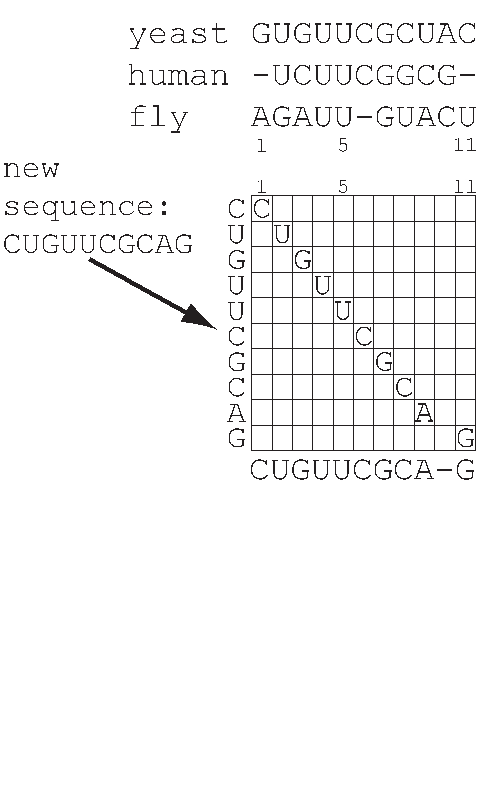
\includegraphics[height=6in]{figs/hmm_alignment2_layer2}
\end{center}
\vspace{1.5in}
\end{minipage}
\end{slide}
%%%%%%%%%%%%%%%%%%%%%%%%%%%%%%%%%%%%%
%%%%%%%%%%%%%%%%%%%%%%%%%%%%%%%%%%%%%%%%%%%%%%%%%%%%%%%%%%%%%%%%%%%%%%%%%%
\begin{slide}
\begin{center}
\large
\textbf{Accelerating CM alignment using HMMs}
\end{center}
\medskip
\begin{minipage}{6in}
\footnotesize
\begin{itemize}
\item
\textbf{main idea:} use fast HMM when it's accurate, appealing to CM when it's not
%main idea: use fast HMM for the regions of the alignment it can get right
%and use slower, more accurate CM for the rest
\item
%requires a method for determining the level of confidence
%(probability) that regions of the HMM alignment are correct 
%need to know the confidence level that regions of the HMM alignment
%are correct
need some type of measure of confidence in regions of the HMM alignment

\end{itemize}
\small
\hspace{0.3in}
\underline{HMM alignment}%\hspace{1.5in}---- $>$
\begin{itemize}
\item
each column of the grid corresponds to a \\ column
of the seed alignment
\item
each row of the grid corresponds to a \\ position of the new sequence
\end{itemize}
\begin{center}
\normalsize
\textbf{How can we use this information during CM alignment?}
\end{center}
\vspace{1.9in}
\end{minipage}
\begin{minipage}{4in}
\begin{center}
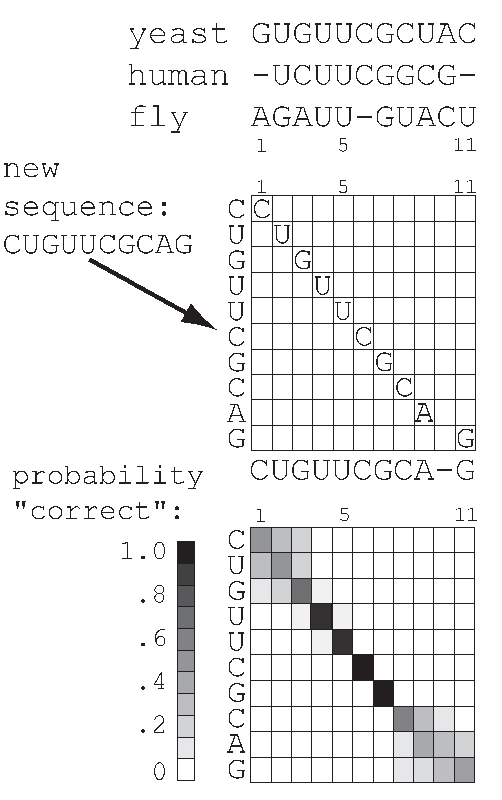
\includegraphics[height=6in]{figs/hmm_alignment2_layer3}
\end{center}
\vspace{1.5in}
\end{minipage}
\end{slide}
%%%%%%%%%%%%%%%%%%%%%%%%%%%%%%%%%%%%%

%%%%%%%%%%%%%%%%%%%%%%%%%%%%%%%%%%%%%%%%%%%%%%%%%%%%%%%%%%%%%%%%%%%%%%%%%%
\begin{slide}
\begin{center}
\large
\textbf{Banded CM alignment}
%\textbf{How can we use this information during CM alignment?}
%\textbf{Accelerating CM alignment using HMMs}
\end{center}
\medskip
%\begin{minipage}{6in}
%\begin{center}
%\normalsize
%\textbf{How can we use this information during CM alignment?}
%\end{center}
\small
\begin{itemize}
\item
\textbf{main idea:} eliminate potential alignments the HMM tells us are very improbable
%\item
%restrict which cells of the CM dynamic programming matrix are filled in
%\item
%requires some type of \textbf{map} from the HMM to the CM
%\item
%each single stranded column or base pair from the seed alignment
%corresponds to \\ a face of the 3D CM dynamic programming matrix
\end{itemize}
\begin{center}
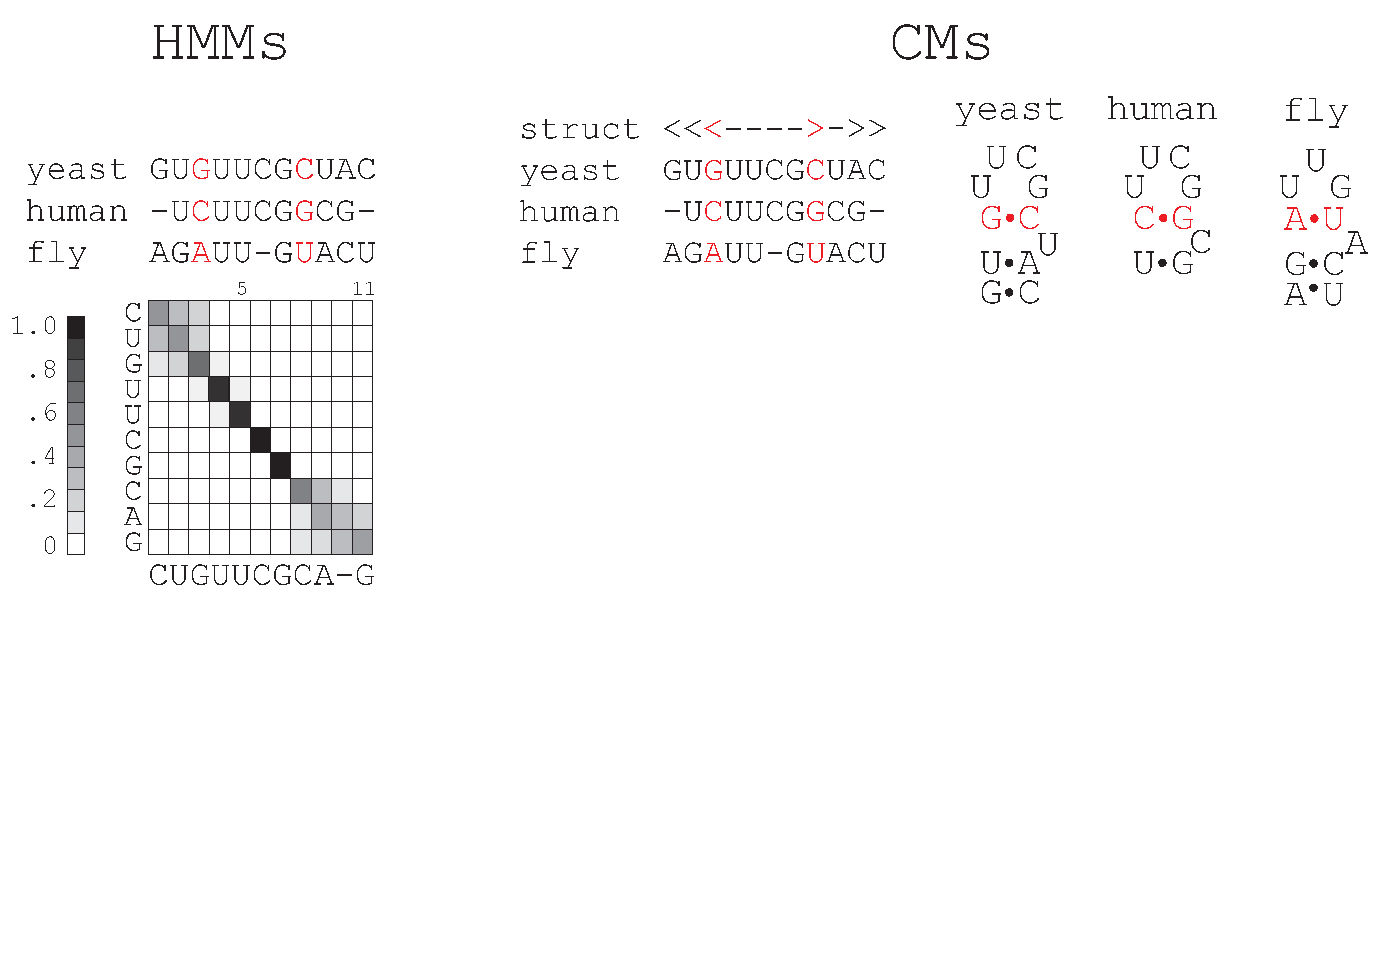
\includegraphics[width=8in]{figs/post_hmm_to_cm_map2_layer1}
\end{center}
\vfill
%\end{minipage}
%\begin{minipage}{4in}
%\vspace{.5in}
%\end{minipage}
\end{slide}
%%%%%%%%%%%%%%%%%%%%%%%%%%%%%%%%%%%%%
%%%%%%%%%%%%%%%%%%%%%%%%%%%%%%%%%%%%%%%%%%%%%%%%%%%%%%%%%%%%%%%%%%%%%%%%%%
\begin{slide}
\begin{center}
\large
\textbf{Banded CM alignment}
%\textbf{How can we use this information during CM alignment?}
%\textbf{Accelerating CM alignment using HMMs}
\end{center}
\medskip
%\begin{minipage}{6in}
%\begin{center}
%\normalsize
%\textbf{How can we use this information during CM alignment?}
%\end{center}
\small
\begin{itemize}
\item
\textbf{main idea:} eliminate potential alignments the HMM tells us are very improbable
%\item
%restrict which cells of the CM dynamic programming matrix are filled in
%\item
%requires some type of \textbf{map} from the HMM to the CM
%\item
%each single stranded column or base pair from the seed alignment
%corresponds to \\ a face of the 3D CM dynamic programming matrix
\end{itemize}
\begin{center}
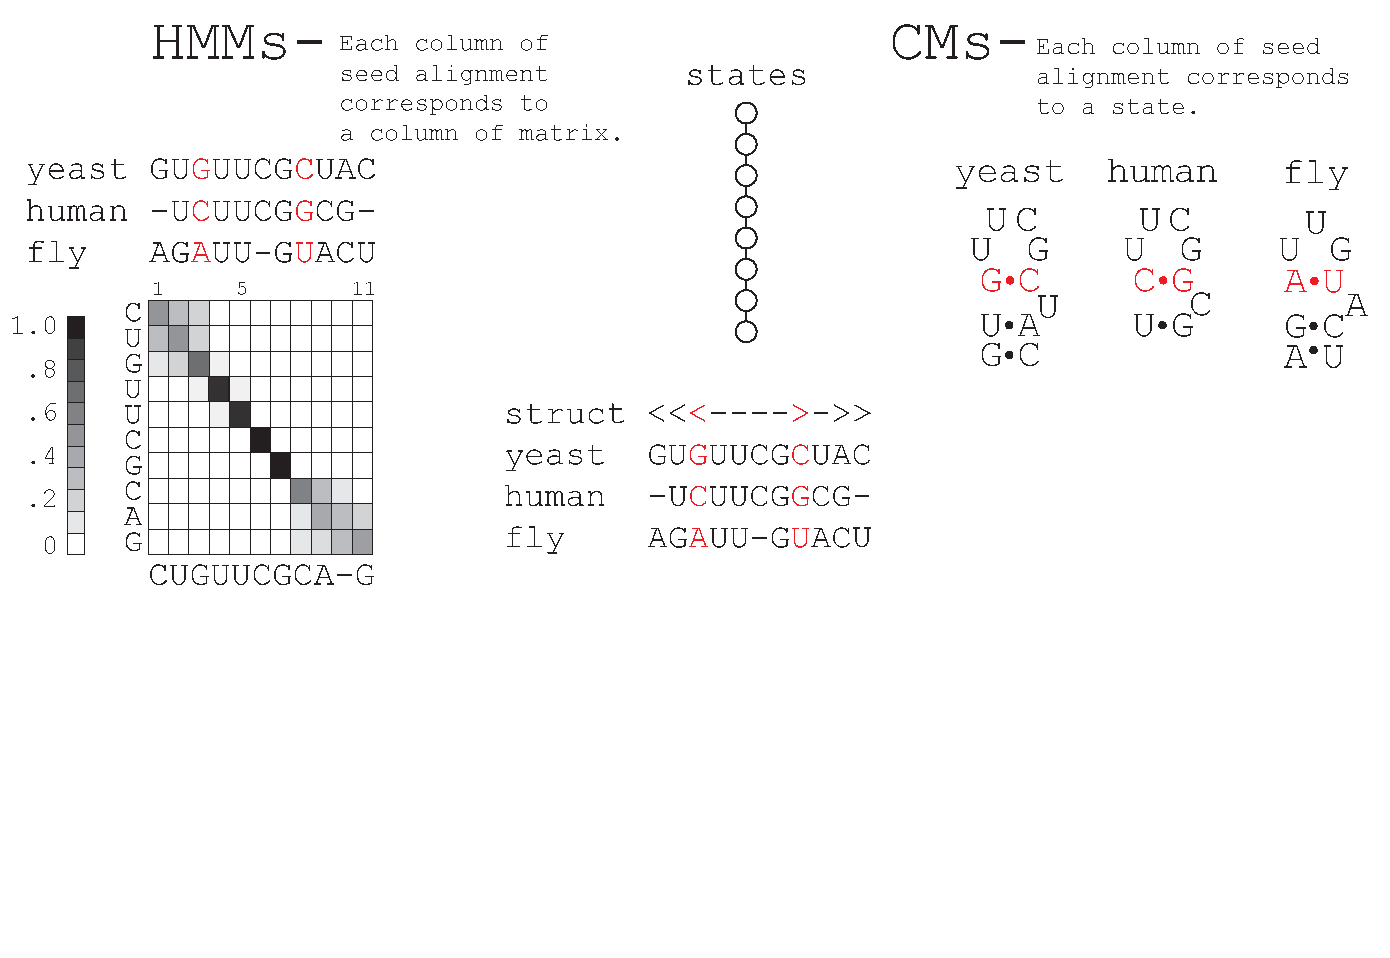
\includegraphics[width=8in]{figs/post_hmm_to_cm_map2_layer2}
\end{center}
\vfill
%\end{minipage}
%\begin{minipage}{4in}
%\vspace{.5in}
%\end{minipage}
\end{slide}
%%%%%%%%%%%%%%%%%%%%%%%%%%%%%%%%%%%%%
%%%%%%%%%%%%%%%%%%%%%%%%%%%%%%%%%%%%%%%%%%%%%%%%%%%%%%%%%%%%%%%%%%%%%%%%%%
\begin{slide}
\begin{center}
\large
\textbf{Banded CM alignment}
%\textbf{How can we use this information during CM alignment?}
%\textbf{Accelerating CM alignment using HMMs}
\end{center}
\medskip
%\begin{minipage}{6in}
%\begin{center}
%\normalsize
%\textbf{How can we use this information during CM alignment?}
%\end{center}
\small
\begin{itemize}
\item
\textbf{main idea:} eliminate potential alignments the HMM tells us are very improbable
%\item
%restrict which cells of the CM dynamic programming matrix are filled in
%\item
%requires some type of \textbf{map} from the HMM to the CM
%\item
%each single stranded column or base pair from the seed alignment
%corresponds to \\ a face of the 3D CM dynamic programming matrix
\end{itemize}
\begin{center}
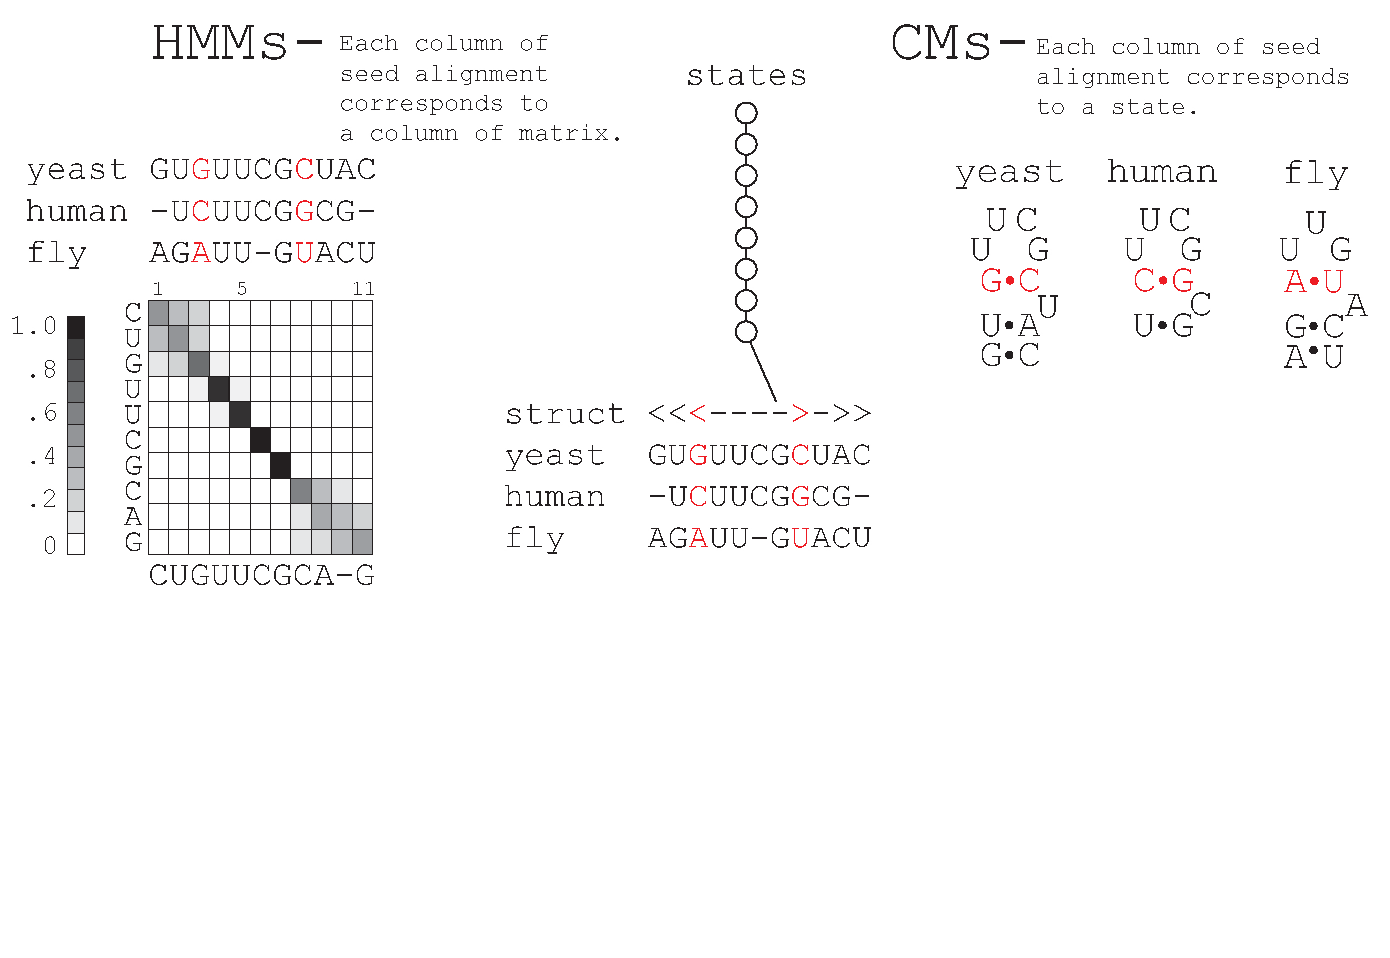
\includegraphics[width=8in]{figs/post_hmm_to_cm_map2_layer3}
\end{center}
\vfill
%\end{minipage}
%\begin{minipage}{4in}
%\vspace{.5in}
%\end{minipage}
\end{slide}
%%%%%%%%%%%%%%%%%%%%%%%%%%%%%%%%%%%%%%%%%%%%%%%%%%%%%%%%%%%%%%%%%%%%%%%%%%
%%%%%%%%%%%%%%%%%%%%%%%%%%%%%%%%%%%%%%%%%%%%%%%%%%%%%%%%%%%%%%%%%%%%%%%%%%
\begin{slide}
\begin{center}
\large
\textbf{Banded CM alignment}
%\textbf{How can we use this information during CM alignment?}
%\textbf{Accelerating CM alignment using HMMs}
\end{center}
\medskip
%\begin{minipage}{6in}
%\begin{center}
%\normalsize
%\textbf{How can we use this information during CM alignment?}
%\end{center}
\small
\begin{itemize}
\item
\textbf{main idea:} eliminate potential alignments the HMM tells us are very improbable
%\item
%restrict which cells of the CM dynamic programming matrix are filled in
%\item
%requires some type of \textbf{map} from the HMM to the CM
%\item
%each single stranded column or base pair from the seed alignment
%corresponds to \\ a face of the 3D CM dynamic programming matrix
\end{itemize}
\begin{center}
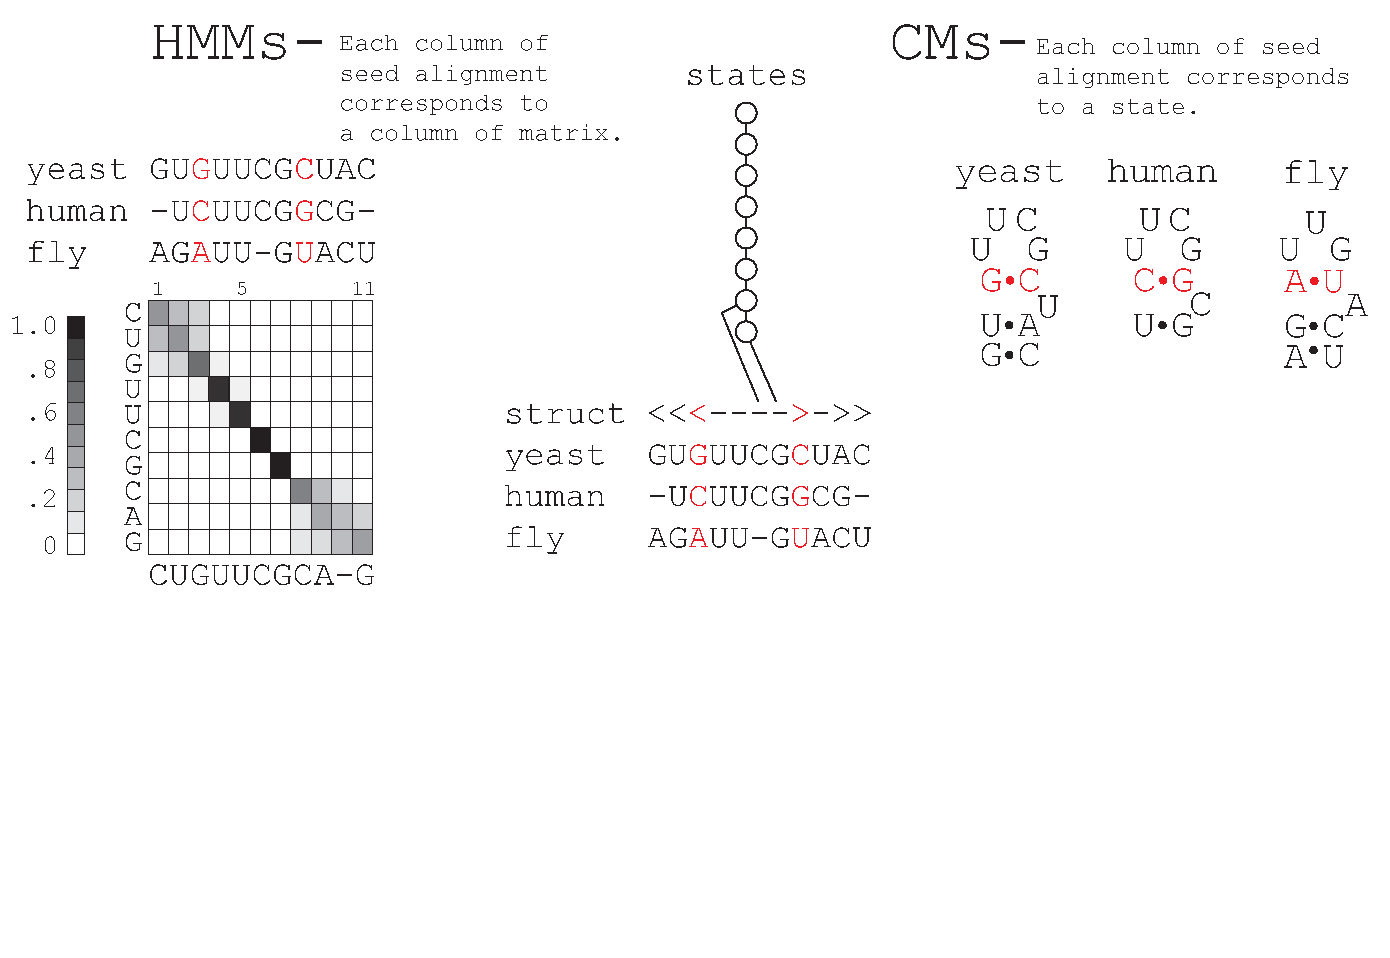
\includegraphics[width=8in]{figs/post_hmm_to_cm_map2_layer4}
\end{center}
\vfill
%\end{minipage}
%\begin{minipage}{4in}
%\vspace{.5in}
%\end{minipage}
\end{slide}
%%%%%%%%%%%%%%%%%%%%%%%%%%%%%%%%%%%%%%%%%%%%%%%%%%%%%%%%%%%%%%%%%%%%%%%%%%
%%%%%%%%%%%%%%%%%%%%%%%%%%%%%%%%%%%%%%%%%%%%%%%%%%%%%%%%%%%%%%%%%%%%%%%%%%
\begin{slide}
\begin{center}
\large
\textbf{Banded CM alignment}
%\textbf{How can we use this information during CM alignment?}
%\textbf{Accelerating CM alignment using HMMs}
\end{center}
\medskip
%\begin{minipage}{6in}
%\begin{center}
%\normalsize
%\textbf{How can we use this information during CM alignment?}
%\end{center}
\small
\begin{itemize}
\item
\textbf{main idea:} eliminate potential alignments the HMM tells us are very improbable
%\item
%restrict which cells of the CM dynamic programming matrix are filled in
%\item
%requires some type of \textbf{map} from the HMM to the CM
%\item
%each single stranded column or base pair from the seed alignment
%corresponds to \\ a face of the 3D CM dynamic programming matrix
\end{itemize}
\begin{center}
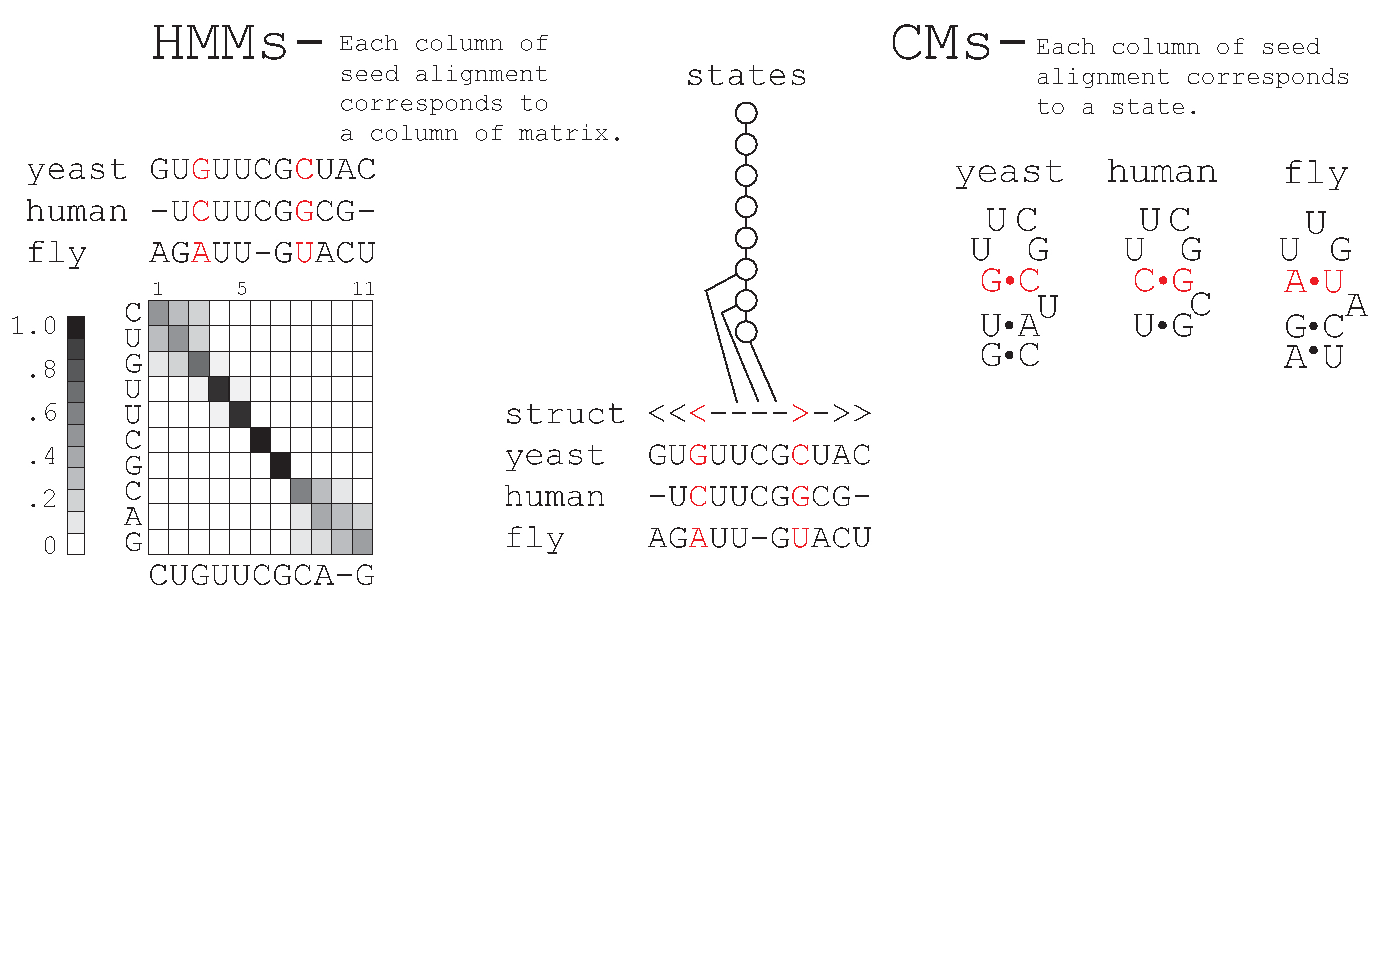
\includegraphics[width=8in]{figs/post_hmm_to_cm_map2_layer5}
\end{center}
\vfill
%\end{minipage}
%\begin{minipage}{4in}
%\vspace{.5in}
%\end{minipage}
\end{slide}
%%%%%%%%%%%%%%%%%%%%%%%%%%%%%%%%%%%%%%%%%%%%%%%%%%%%%%%%%%%%%%%%%%%%%%%%%%
%%%%%%%%%%%%%%%%%%%%%%%%%%%%%%%%%%%%%%%%%%%%%%%%%%%%%%%%%%%%%%%%%%%%%%%%%%
\begin{slide}
\begin{center}
\large
\textbf{Banded CM alignment}
%\textbf{How can we use this information during CM alignment?}
%\textbf{Accelerating CM alignment using HMMs}
\end{center}
\medskip
%\begin{minipage}{6in}
%\begin{center}
%\normalsize
%\textbf{How can we use this information during CM alignment?}
%\end{center}
\small
\begin{itemize}
\item
\textbf{main idea:} eliminate potential alignments the HMM tells us are very improbable
%\item
%restrict which cells of the CM dynamic programming matrix are filled in
%\item
%requires some type of \textbf{map} from the HMM to the CM
%\item
%each single stranded column or base pair from the seed alignment
%corresponds to \\ a face of the 3D CM dynamic programming matrix
\end{itemize}
\begin{center}
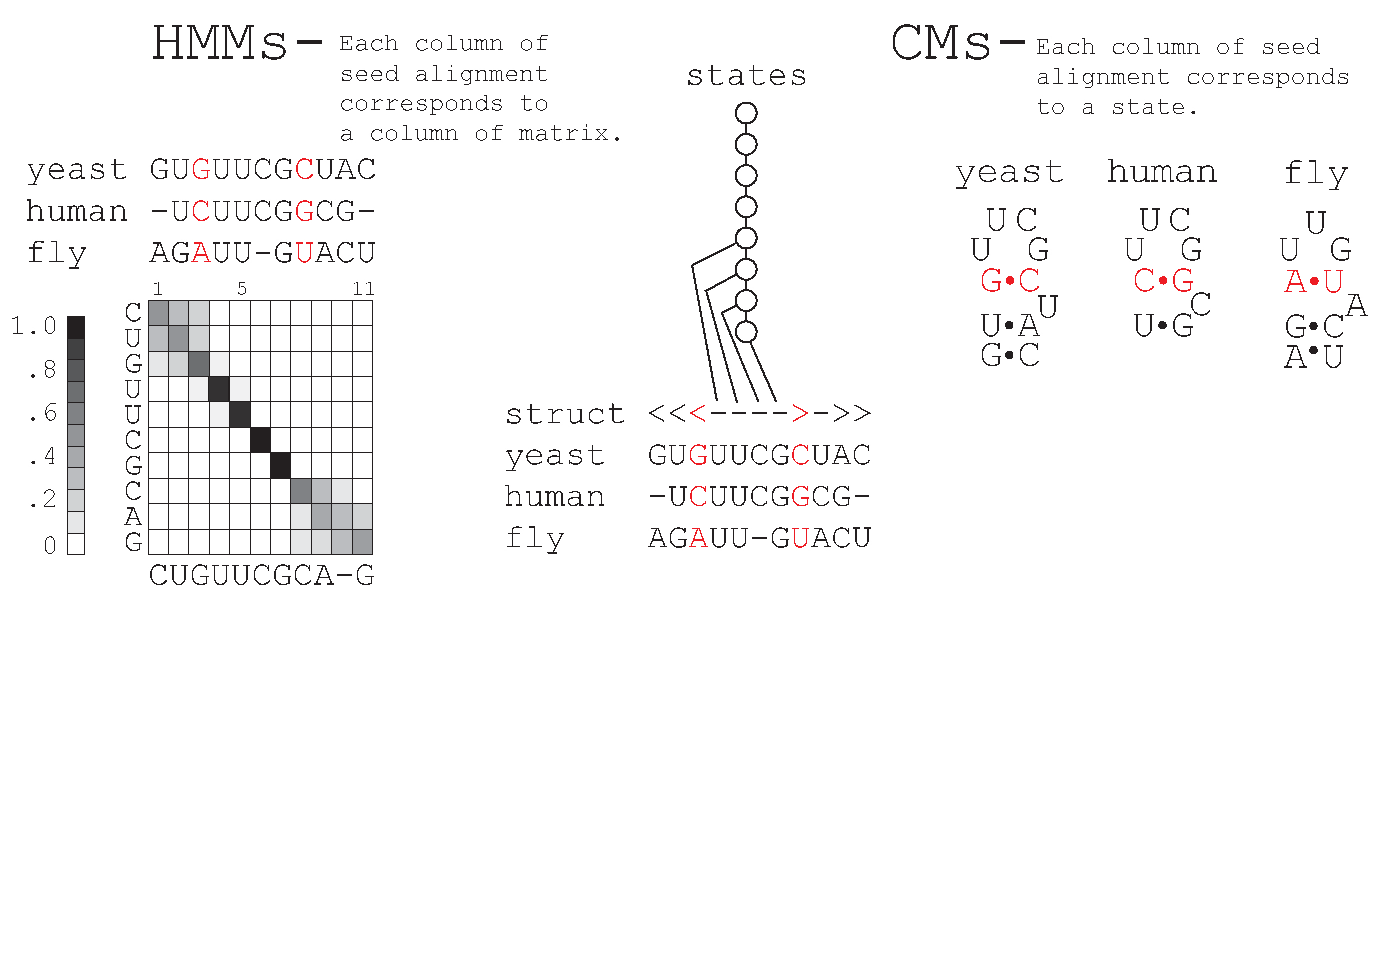
\includegraphics[width=8in]{figs/post_hmm_to_cm_map2_layer6}
\end{center}
\vfill
%\end{minipage}
%\begin{minipage}{4in}
%\vspace{.5in}
%\end{minipage}
\end{slide}
%%%%%%%%%%%%%%%%%%%%%%%%%%%%%%%%%%%%%%%%%%%%%%%%%%%%%%%%%%%%%%%%%%%%%%%%%%
%%%%%%%%%%%%%%%%%%%%%%%%%%%%%%%%%%%%%%%%%%%%%%%%%%%%%%%%%%%%%%%%%%%%%%%%%%
\begin{slide}
\begin{center}
\large
\textbf{Banded CM alignment}
%\textbf{How can we use this information during CM alignment?}
%\textbf{Accelerating CM alignment using HMMs}
\end{center}
\medskip
%\begin{minipage}{6in}
%\begin{center}
%\normalsize
%\textbf{How can we use this information during CM alignment?}
%\end{center}
\small
\begin{itemize}
\item
\textbf{main idea:} eliminate potential alignments the HMM tells us are very improbable
%\item
%restrict which cells of the CM dynamic programming matrix are filled in
%\item
%requires some type of \textbf{map} from the HMM to the CM
%\item
%each single stranded column or base pair from the seed alignment
%corresponds to \\ a face of the 3D CM dynamic programming matrix
\end{itemize}
\begin{center}
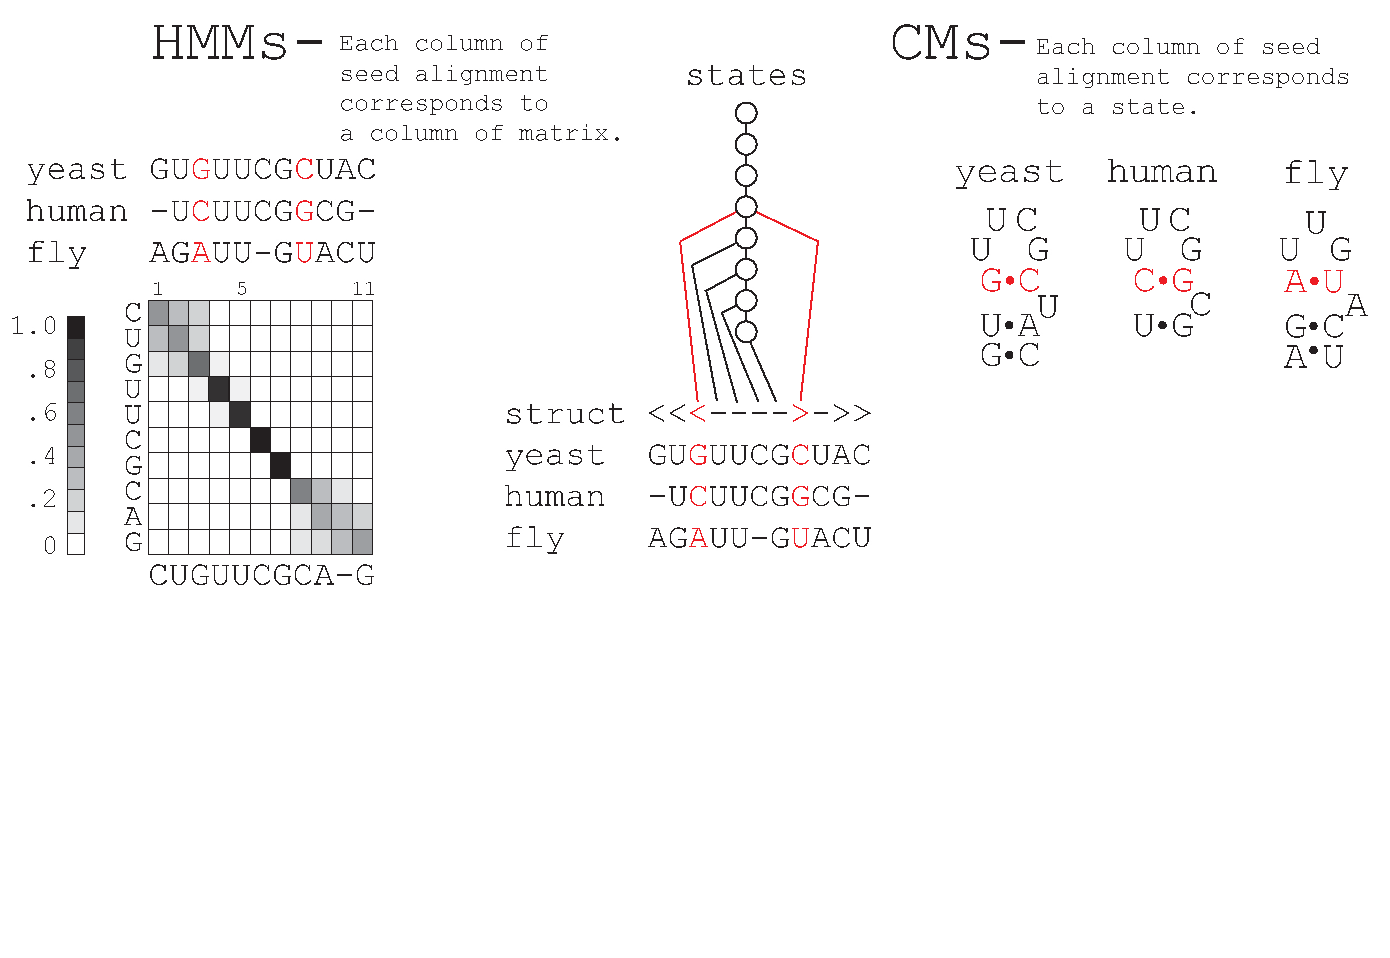
\includegraphics[width=8in]{figs/post_hmm_to_cm_map2_layer7}
\end{center}
\vfill
%\end{minipage}
%\begin{minipage}{4in}
%\vspace{.5in}
%\end{minipage}
\end{slide}
%%%%%%%%%%%%%%%%%%%%%%%%%%%%%%%%%%%%%%%%%%%%%%%%%%%%%%%%%%%%%%%%%%%%%%%%%%
%%%%%%%%%%%%%%%%%%%%%%%%%%%%%%%%%%%%%%%%%%%%%%%%%%%%%%%%%%%%%%%%%%%%%%%%%%
\begin{slide}
\begin{center}
\large
\textbf{Banded CM alignment}
%\textbf{How can we use this information during CM alignment?}
%\textbf{Accelerating CM alignment using HMMs}
\end{center}
\medskip
%\begin{minipage}{6in}
%\begin{center}
%\normalsize
%\textbf{How can we use this information during CM alignment?}
%\end{center}
\small
\begin{itemize}
\item
\textbf{main idea:} eliminate potential alignments the HMM tells us are very improbable
%\item
%restrict which cells of the CM dynamic programming matrix are filled in
%\item
%requires some type of \textbf{map} from the HMM to the CM
%\item
%each single stranded column or base pair from the seed alignment
%corresponds to \\ a face of the 3D CM dynamic programming matrix
\end{itemize}
\begin{center}
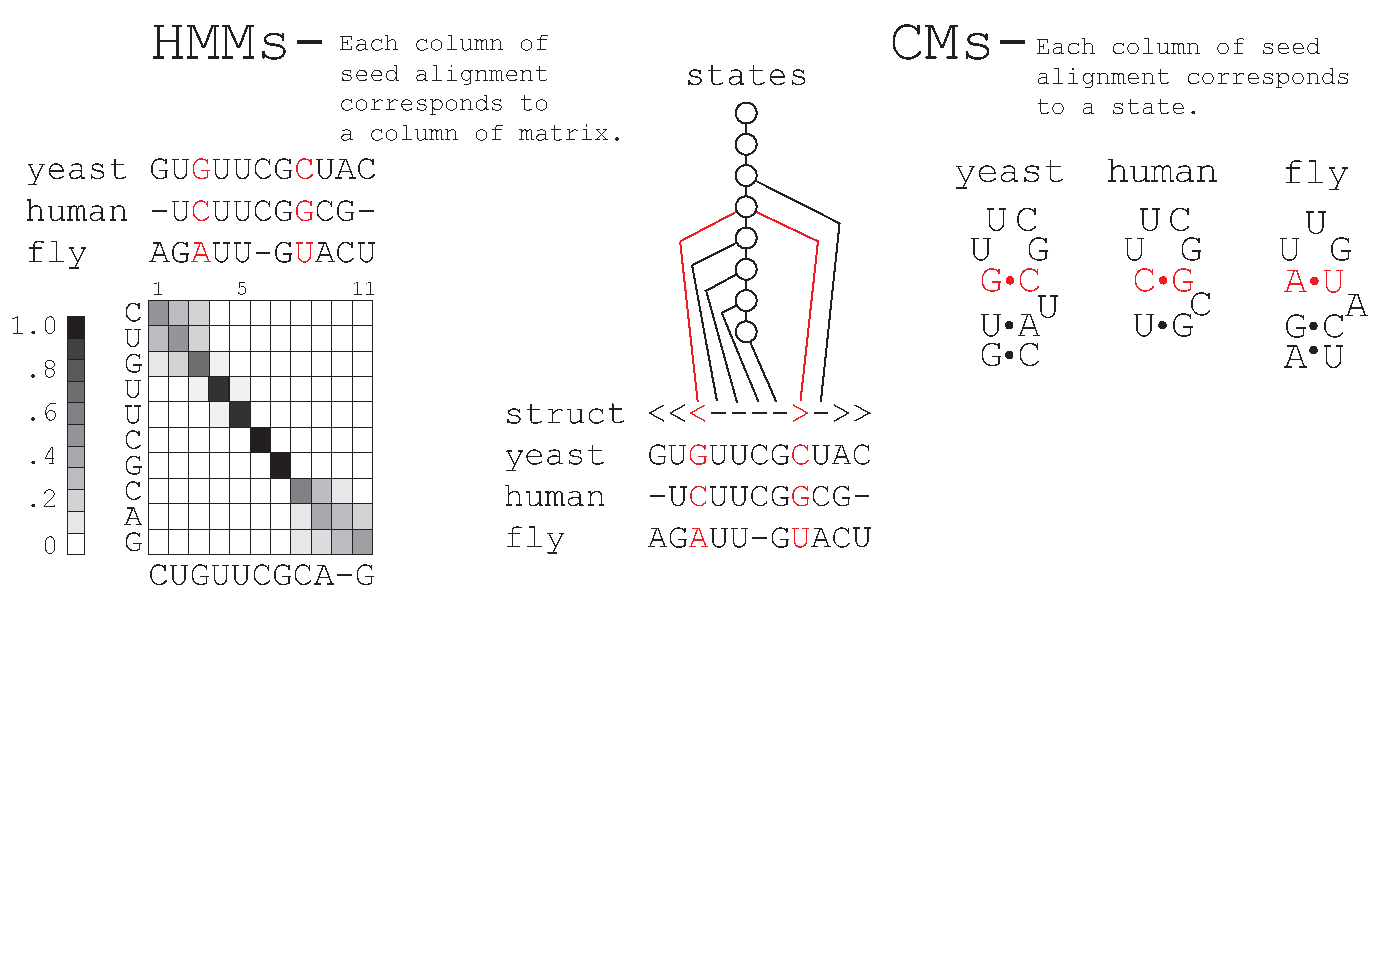
\includegraphics[width=8in]{figs/post_hmm_to_cm_map2_layer8}
\end{center}
\vfill
%\end{minipage}
%\begin{minipage}{4in}
%\vspace{.5in}
%\end{minipage}
\end{slide}
%%%%%%%%%%%%%%%%%%%%%%%%%%%%%%%%%%%%%%%%%%%%%%%%%%%%%%%%%%%%%%%%%%%%%%%%%%
%%%%%%%%%%%%%%%%%%%%%%%%%%%%%%%%%%%%%%%%%%%%%%%%%%%%%%%%%%%%%%%%%%%%%%%%%%
\begin{slide}
\begin{center}
\large
\textbf{Banded CM alignment}
%\textbf{How can we use this information during CM alignment?}
%\textbf{Accelerating CM alignment using HMMs}
\end{center}
\medskip
%\begin{minipage}{6in}
%\begin{center}
%\normalsize
%\textbf{How can we use this information during CM alignment?}
%\end{center}
\small
\begin{itemize}
\item
\textbf{main idea:} eliminate potential alignments the HMM tells us are very improbable
%\item
%restrict which cells of the CM dynamic programming matrix are filled in
%\item
%requires some type of \textbf{map} from the HMM to the CM
%\item
%each single stranded column or base pair from the seed alignment
%corresponds to \\ a face of the 3D CM dynamic programming matrix
\end{itemize}
\begin{center}
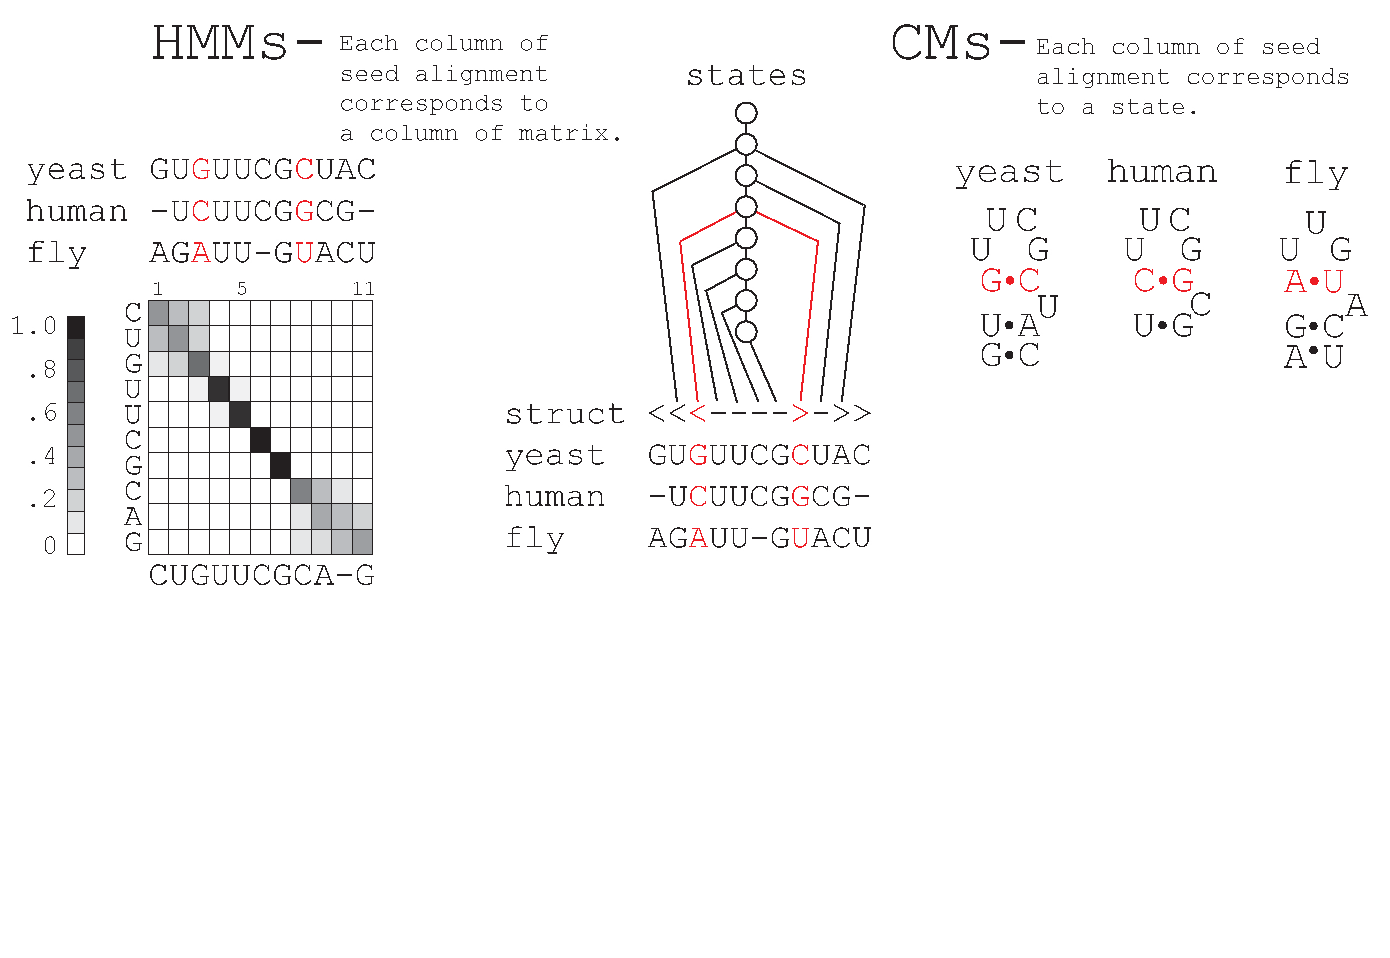
\includegraphics[width=8in]{figs/post_hmm_to_cm_map2_layer9}
\end{center}
\vfill
%\end{minipage}
%\begin{minipage}{4in}
%\vspace{.5in}
%\end{minipage}
\end{slide}
%%%%%%%%%%%%%%%%%%%%%%%%%%%%%%%%%%%%%%%%%%%%%%%%%%%%%%%%%%%%%%%%%%%%%%%%%%
%%%%%%%%%%%%%%%%%%%%%%%%%%%%%%%%%%%%%%%%%%%%%%%%%%%%%%%%%%%%%%%%%%%%%%%%%%
\begin{slide}
\begin{center}
\large
\textbf{Banded CM alignment}
%\textbf{How can we use this information during CM alignment?}
%\textbf{Accelerating CM alignment using HMMs}
\end{center}
\medskip
%\begin{minipage}{6in}
%\begin{center}
%\normalsize
%\textbf{How can we use this information during CM alignment?}
%\end{center}
\small
\begin{itemize}
\item
\textbf{main idea:} eliminate potential alignments the HMM tells us are very improbable
%\item
%restrict which cells of the CM dynamic programming matrix are filled in
%\item
%requires some type of \textbf{map} from the HMM to the CM
%\item
%each single stranded column or base pair from the seed alignment
%corresponds to \\ a face of the 3D CM dynamic programming matrix
\end{itemize}
\begin{center}
\includegraphics[width=8in]{figs/post_hmm_to_cm_map2_layer10}
\end{center}
\vfill
%\end{minipage}
%\begin{minipage}{4in}
%\vspace{.5in}
%\end{minipage}
\end{slide}
%%%%%%%%%%%%%%%%%%%%%%%%%%%%%%%%%%%%%%%%%%%%%%%%%%%%%%%%%%%%%%%%%%%%%%%%%%
%%%%%%%%%%%%%%%%%%%%%%%%%%%%%%%%%%%%%%%%%%%%%%%%%%%%%%%%%%%%%%%%%%%%%%%%%%
\begin{slide}
\begin{center}
\large
\textbf{Banded CM alignment}
%\textbf{How can we use this information during CM alignment?}
%\textbf{Accelerating CM alignment using HMMs}
\end{center}
\medskip
%\begin{minipage}{6in}
%\begin{center}
%\normalsize
%\textbf{How can we use this information during CM alignment?}
%\end{center}
\small
\begin{itemize}
\item
\textbf{main idea:} eliminate potential alignments the HMM tells us are very improbable
%\item
%restrict which cells of the CM dynamic programming matrix are filled in
%\item
%requires some type of \textbf{map} from the HMM to the CM
%\item
%each single stranded column or base pair from the seed alignment
%corresponds to \\ a face of the 3D CM dynamic programming matrix
\end{itemize}
\begin{center}
\includegraphics[width=8in]{figs/post_hmm_to_cm_map2_layer11}
\end{center}
\vfill
%\end{minipage}
%\begin{minipage}{4in}
%\vspace{.5in}
%\end{minipage}
\end{slide}
%%%%%%%%%%%%%%%%%%%%%%%%%%%%%%%%%%%%%%%%%%%%%%%%%%%%%%%%%%%%%%%%%%%%%%%%%%
%%%%%%%%%%%%%%%%%%%%%%%%%%%%%%%%%%%%%%%%%%%%%%%%%%%%%%%%%%%%%%%%%%%%%%%%%%
\begin{slide}
\begin{center}
\large
\textbf{Banded CM alignment}
%\textbf{How can we use this information during CM alignment?}
%\textbf{Accelerating CM alignment using HMMs}
\end{center}
\medskip
%\begin{minipage}{6in}
%\begin{center}
%\normalsize
%\textbf{How can we use this information during CM alignment?}
%\end{center}
\small
\begin{itemize}
\item
\textbf{main idea:} eliminate potential alignments the HMM tells us are very improbable
%\item
%restrict which cells of the CM dynamic programming matrix are filled in
%\item
%requires some type of \textbf{map} from the HMM to the CM
%\item
%each single stranded column or base pair from the seed alignment
%corresponds to \\ a face of the 3D CM dynamic programming matrix
\end{itemize}
\begin{center}
\includegraphics[width=8in]{figs/post_hmm_to_cm_map2_layer12}
\end{center}
\vfill
%\end{minipage}
%\begin{minipage}{4in}
%\vspace{.5in}
%\end{minipage}
\end{slide}
%%%%%%%%%%%%%%%%%%%%%%%%%%%%%%%%%%%%%%%%%%%%%%%%%%%%%%%%%%%%%%%%%%%%%%%%%%
%%%%%%%%%%%%%%%%%%%%%%%%%%%%%%%%%%%%%%%%%%%%%%%%%%%%%%%%%%%%%%%%%%%%%%%%%%
\begin{slide}
\begin{center}
\large
\textbf{Banded CM alignment}
%\textbf{How can we use this information during CM alignment?}
%\textbf{Accelerating CM alignment using HMMs}
\end{center}
\medskip
%\begin{minipage}{6in}
%\begin{center}
%\normalsize
%\textbf{How can we use this information during CM alignment?}
%\end{center}
\small
\begin{itemize}
\item
\textbf{main idea:} eliminate potential alignments the HMM tells us are very improbable
%\item
%restrict which cells of the CM dynamic programming matrix are filled in
%\item
%requires some type of \textbf{map} from the HMM to the CM
%\item
%each single stranded column or base pair from the seed alignment
%corresponds to \\ a face of the 3D CM dynamic programming matrix
\end{itemize}
\begin{center}
\includegraphics[width=8in]{figs/post_hmm_to_cm_map2_layer13}
\end{center}
\vfill
%\end{minipage}
%\begin{minipage}{4in}
%\vspace{.5in}
%\end{minipage}
\end{slide}
%%%%%%%%%%%%%%%%%%%%%%%%%%%%%%%%%%%%%%%%%%%%%%%%%%%%%%%%%%%%%%%%%%%%%%%%%%
%%%%%%%%%%%%%%%%%%%%%%%%%%%%%%%%%%%%%%%%%%%%%%%%%%%%%%%%%%%%%%%%%%%%%%%%%%
\begin{slide}
\begin{center}
\large
\textbf{Banded CM alignment}
%\textbf{How can we use this information during CM alignment?}
%\textbf{Accelerating CM alignment using HMMs}
\end{center}
\medskip
%\begin{minipage}{6in}
%\begin{center}
%\normalsize
%\textbf{How can we use this information during CM alignment?}
%\end{center}
\small
\begin{itemize}
\item
\textbf{main idea:} eliminate potential alignments the HMM tells us are very improbable
%\item
%restrict which cells of the CM dynamic programming matrix are filled in
%\item
%requires some type of \textbf{map} from the HMM to the CM
%\item
%each single stranded column or base pair from the seed alignment
%corresponds to \\ a face of the 3D CM dynamic programming matrix
\end{itemize}
\begin{center}
\includegraphics[width=8in]{figs/post_hmm_to_cm_map2_layer14}
\end{center}
\vfill
%\end{minipage}
%\begin{minipage}{4in}
%\vspace{.5in}
%\end{minipage}
\end{slide}
%%%%%%%%%%%%%%%%%%%%%%%%%%%%%%%%%%%%%%%%%%%%%%%%%%%%%%%%%%%%%%%%%%%%%%%%%%
%%%%%%%%%%%%%%%%%%%%%%%%%%%%%%%%%%%%%%%%%%%%%%%%%%%%%%%%%%%%%%%%%%%%%%%%%%
\begin{slide}
\begin{center}
\large
\textbf{Banded CM alignment}
%\textbf{How can we use this information during CM alignment?}
%\textbf{Accelerating CM alignment using HMMs}
\end{center}
\medskip
%\begin{minipage}{6in}
%\begin{center}
%\normalsize
%\textbf{How can we use this information during CM alignment?}
%\end{center}
\small
\begin{itemize}
\item
\textbf{main idea:} eliminate potential alignments the HMM tells us are very improbable
%\item
%restrict which cells of the CM dynamic programming matrix are filled in
%\item
%requires some type of \textbf{map} from the HMM to the CM
%\item
%each single stranded column or base pair from the seed alignment
%corresponds to \\ a face of the 3D CM dynamic programming matrix
\end{itemize}
\begin{center}
\includegraphics[width=8in]{figs/post_hmm_to_cm_map2_layer15}
\end{center}
\vfill
%\end{minipage}
%\begin{minipage}{4in}
%\vspace{.5in}
%\end{minipage}
\end{slide}
%%%%%%%%%%%%%%%%%%%%%%%%%%%%%%%%%%%%%%%%%%%%%%%%%%%%%%%%%%%%%%%%%%%%%%%%%%
%%%%%%%%%%%%%%%%%%%%%%%%%%%%%%%%%%%%%%%%%%%%%%%%%%%%%%%%%%%%%%%%%%%%%%%%%%
\begin{slide}
\begin{center}
\large
\textbf{Banded CM alignment}
%\textbf{How can we use this information during CM alignment?}
%\textbf{Accelerating CM alignment using HMMs}
\end{center}
\medskip
%\begin{minipage}{6in}
%\begin{center}
%\normalsize
%\textbf{How can we use this information during CM alignment?}
%\end{center}
\small
\begin{itemize}
\item
\textbf{main idea:} eliminate potential alignments the HMM tells us are very improbable
%\item
%restrict which cells of the CM dynamic programming matrix are filled in
%\item
%requires some type of \textbf{map} from the HMM to the CM
%\item
%each single stranded column or base pair from the seed alignment
%corresponds to \\ a face of the 3D CM dynamic programming matrix
\end{itemize}
\begin{center}
\includegraphics[width=8in]{figs/post_hmm_to_cm_map2_layer16}
\end{center}
\vfill
%\end{minipage}
%\begin{minipage}{4in}
%\vspace{.5in}
%\end{minipage}
\end{slide}
%%%%%%%%%%%%%%%%%%%%%%%%%%%%%%%%%%%%%%%%%%%%%%%%%%%%%%%%%%%%%%%%%%%%%%%%%%
%%%%%%%%%%%%%%%%%%%%%%%%%%%%%%%%%%%%%%%%%%%%%%%%%%%%%%%%%%%%%%%%%%%
\begin{slide}
\begin{center}
\large
\textbf{Benchmarking SSU alignment}
\end{center}
\medskip

\small
\begin{itemize}
\item
Does the banded CM approach sacrifice accuracy relative to
non-banded CM alignment?
%\item
%How accurately do profiles align SSU?
%\end{itemize}
\item
'Gold standard' testing dataset
\begin{itemize}
\item
structural alignment of 152 bacterial SSU sequences
from Robin Gutell's database
%the Comparative RNA Website (CRW)
%structural alignment of 221 bacterial SSU sequences
%from the Comparative RNA Website (CRW)
\item
this is the CRW bacterial seed alignment filtered to 92\% identity
\item
determined by 'manual' comparative analysis
\begin{comment}
\item
152 deep alignment is clustered into two groups based on sequence identity:
%representative subset of 46 sequences used as the seed alignment
%(no two are $>$ 80\% identical)
\begin{itemize}
\item
training (seed) alignment of 101 sequences
\item
testing alignment of 51 sequences
\item
  no train/test pair is > 80\% identical
\end{itemize}
\item
Benchmark: train profile on 101-deep seed and test alignment accuracy on the remaining 175 sequences
\end{comment}

%measure accuracy of predicted base pairs versus correct base pairs
\end{itemize}
\end{itemize}

\center{\includegraphics[width=10.5in]{figs/diana_benchmark_l1}}

\vfill
\end{slide}
%%%%%%%%%%%%%%%%%%%%%%%%%%%%%%%%%%%%%%%%%%%%%%%%%%%%%%%%%%%%%%%%%%%%%%%%%
%%%%%%%%%%%%%%%%%%%%%%%%%%%%%%%%%%%%%%%%%%%%%%%%%%%%%%%%%%%%%%%%%%%
\begin{slide}
\begin{center}
\large
\textbf{Benchmarking SSU alignment}
\end{center}
\medskip

\small
\begin{itemize}
\item
Does the banded CM approach sacrifice accuracy relative to
non-banded CM alignment?
%\item
%How accurately do profiles align SSU?
%\end{itemize}
\item
'Gold standard' testing dataset
\begin{itemize}
\item
structural alignment of 152 bacterial SSU sequences
from Robin Gutell's database
%the Comparative RNA Website (CRW)
%structural alignment of 221 bacterial SSU sequences
%from the Comparative RNA Website (CRW)
\item
this is the CRW bacterial seed alignment filtered to 92\% identity
\item
determined by 'manual' comparative analysis
\begin{comment}
\item
152 deep alignment is clustered into two groups based on sequence identity:
%representative subset of 46 sequences used as the seed alignment
%(no two are $>$ 80\% identical)
\begin{itemize}
\item
training (seed) alignment of 101 sequences
\item
testing alignment of 51 sequences
\item
  no train/test pair is > 80\% identical
\end{itemize}
\item
Benchmark: train profile on 101-deep seed and test alignment accuracy on the remaining 175 sequences
\end{comment}

%measure accuracy of predicted base pairs versus correct base pairs
\end{itemize}
\end{itemize}

\center{\includegraphics[width=10.5in]{figs/diana_benchmark_l2}}

\vfill
\end{slide}
%%%%%%%%%%%%%%%%%%%%%%%%%%%%%%%%%%%%%%%%%%%%%%%%%%%%%%%%%%%%%%%%%%%%%%%%%
\begin{slide}
\begin{center}
\large
\textbf{Results}
\end{center}
\medskip
\medskip
\begin{center}

\begin{tabular}{rcr} 
& \multicolumn{1}{c}{alignment} & \multicolumn{1}{c}{time} \\
& \multicolumn{1}{c}{accuracy} & \multicolumn{1}{c}{(sec/seq)} \\ \hline
& \multicolumn{1}{c}{} & \multicolumn{1}{c}{} \\
clustalw & 92.2\% & 30.0 \\ 
& \multicolumn{1}{c}{} & \multicolumn{1}{c}{} \\
HMMs & 96.2\% & 0.08 \\ 
& \multicolumn{1}{c}{} & \multicolumn{1}{c}{} \\
non-banded CMs & 97.8\% & 795.0 \\ 
& \multicolumn{1}{c}{} & \multicolumn{1}{c}{} \\
HMM banded CMs & 97.8\% & 1.3 \\ %1.1
& \multicolumn{1}{c}{} & \multicolumn{1}{c}{} \\
probabilistically masked & & \\
HMM banded CMs           & 99.7\% & 1.3 \\ %1.1
& \multicolumn{1}{c}{} & \multicolumn{1}{c}{} \\
\end{tabular}
\end{center}

\vfill
\end{slide}
%%%%%%%%%%%%%%%%%%%%%%%%%%%%%%%%%%%%%%%%%%%%%%%%%%%%%%%%%%%%%%%%%%%%%%%%%
% Results pre 09.19.07 (reported in Venter, AG, Friday talk)
%HMMs & 96.62\% & 0.1 (pre 09.19.07) 
%non-banded CMs & 98.19\% & 1407.1 (pre 09.19.07)\\ 
%HMM banded CMs & 98.17\% & 3.5 \\ 
%
%%%%%%%%%%%%%%%%%%%%%%%%%%%%%%%%%%%%%%%%%%%%%%%%%%%%%%%%%%%%%%%%%%%%%%%%%
\begin{slide}
\begin{center}
\large
\textbf{Results}
\end{center}
\medskip
\medskip
\begin{center}

\begin{tabular}{rcr} 
& \multicolumn{1}{c}{alignment} & \multicolumn{1}{c}{time} \\
& \multicolumn{1}{c}{accuracy} & \multicolumn{1}{c}{(sec/seq)} \\ \hline
& \multicolumn{1}{c}{} & \multicolumn{1}{c}{} \\
clustalw & 92.2\% & 30.0 \\ 
& \multicolumn{1}{c}{} & \multicolumn{1}{c}{} \\
HMMs & 96.2\% & 0.08 \\ 
& \multicolumn{1}{c}{} & \multicolumn{1}{c}{} \\
non-banded CMs & 97.8\% & 795.0 \\ 
& \multicolumn{1}{c}{} & \multicolumn{1}{c}{} \\
%HMM banded CMs & 97.8\% & 1.3 \\ %1.1
%& \multicolumn{1}{c}{} & \multicolumn{1}{c}{} \\
\end{tabular}
\end{center}

\vfill
\end{slide}
%%%%%%%%%%%%%%%%%%%%%%%%%%%%%%%%%%%%%%%%%%%%%%%%%%%%%%%%%%%%%%%%%%%%%%%%%
%%%%%%%%%%%%%%%%%%%%%%%%%%%%%%%%%%%%%%%%%%%%%%%%%%%%%%%%%%%%%%%%%%%%%%%%%
\begin{slide}
\begin{center}
\large
\textbf{Results}
\end{center}
\medskip
\medskip
\begin{center}

\begin{tabular}{rcr} 
& \multicolumn{1}{c}{alignment} & \multicolumn{1}{c}{time} \\
& \multicolumn{1}{c}{accuracy} & \multicolumn{1}{c}{(sec/seq)} \\ \hline
& \multicolumn{1}{c}{} & \multicolumn{1}{c}{} \\
clustalw & 92.2\% & 30.0 \\ 
& \multicolumn{1}{c}{} & \multicolumn{1}{c}{} \\
HMMs & 96.2\% & 0.08 \\ 
& \multicolumn{1}{c}{} & \multicolumn{1}{c}{} \\
non-banded CMs & 97.8\% & 795.0 \\ 
& \multicolumn{1}{c}{} & \multicolumn{1}{c}{} \\
HMM banded CMs & 97.8\% & 1.3 \\ %1.1
& \multicolumn{1}{c}{} & \multicolumn{1}{c}{} \\
\end{tabular}
\end{center}

\vfill
\end{slide}
%%%%%%%%%%%%%%%%%%%%%%%%%%%%%%%%%%%%%%%%%%%%%%%%%%%%%%%%%%%%%%%%%%%%%%%%%
\begin{comment}
\begin{slide}
\begin{center}
\large
\textbf{Results}
\end{center}
\medskip
\medskip
\begin{center}

\begin{tabular}{rcr} 
& \multicolumn{1}{c}{alignment} & \multicolumn{1}{c}{time} \\
& \multicolumn{1}{c}{accuracy} & \multicolumn{1}{c}{(sec/seq)} \\ \hline
& \multicolumn{1}{c}{} & \multicolumn{1}{c}{} \\
clustalw & 92.2\% & 30.0 \\ 
& \multicolumn{1}{c}{} & \multicolumn{1}{c}{} \\
HMMs & 96.2\% & 0.08 \\ 
& \multicolumn{1}{c}{} & \multicolumn{1}{c}{} \\
non-banded CMs & 97.8\% & 795.0 \\ 
& \multicolumn{1}{c}{} & \multicolumn{1}{c}{} \\
HMM banded CMs & 97.8\% & 1.3 \\ %1.1
& \multicolumn{1}{c}{} & \multicolumn{1}{c}{} \\
\end{tabular}
\end{center}

\begin{center}
\large
\textbf{HMM banding technique is general}
\end{center}

%\small
%\begin{itemize}
%\item
%  Acceleration is greater for longer families
%\item
%  LSU alignment goes from about 3 hours to 8 seconds
%\end{itemize}

\small
\begin{center}
\begin{tabular}{lrr} 
%        clen    acceleration
%tRNA    72      4.5
%RNaseP  307     31.6
%SSU     1534    793.1  (no --sub) 396.5 (--sub)
%LSU     2916    3465.2 (no --sub)       
%see ~/notebook/7_0919_colorado_talk/00LOG:
  family & length & HMM banding acceleration \\ \hline
  tRNA      & 73   & 4.5 \\
  RNase P   & 307  & 31.6 \\
  SSU rRNA  & 1534 & 600.0 \\ %793.1
  LSU rRNA  & 2914 & 1732.6 \\ %3465.2
\end{tabular}
\end{center}

\vfill
\end{slide}
\end{comment}
%%%%%%%%%%%%%%%%%%%%%%%%%%%%%%%%%%%%%%%%%%%%%%%%%%%%%%%%%%%%%%%%%%%%%%%%%%
%%%%%%%%%%%%%%%%%%%%%%%%%%%%%%%%%%%%%%%%%%%%%%%%%%%%%%%%%%%%%%%%%%%%%%%%%%
\begin{slide}
\begin{center}
\large
\textbf{Phil Hugenholtz's manually created mask}
\end{center}
\small

\begin{center}
\includegraphics[height=7.5in]{figs/lmph-on-1513}

\end{center}
\vfill
\end{slide}
%%%%%%%%%%%%%%%%%%%%%%%%%%%%%%%%%%%%%%%%%%%%%%%%%%%%%%%%%%%%%%%%%%%%%%%%%%%%%%%%%%%%%%%%%%%%%
\begin{slide}\begin{center}\includegraphics[height=8in]{figs/arc-1}\end{center}\vfill\end{slide}
%%%%%%%%%%%%%%%%%%%%%%%%%%%%%%%%%%%%%%%%%%%%%%%%%%%%%%%%%%%%%%%%%%%%%%%%%%%%%%%%%%%%%%%%%%%%%
\begin{slide}\begin{center}\includegraphics[height=8in]{figs/arc-2}\end{center}\vfill\end{slide}
%%%%%%%%%%%%%%%%%%%%%%%%%%%%%%%%%%%%%%%%%%%%%%%%%%%%%%%%%%%%%%%%%%%%%%%%%%%%%%%%%%%%%%%%%%%%%
\begin{slide}\begin{center}\includegraphics[height=8in]{figs/arc-3}\end{center}\vfill\end{slide}
%%%%%%%%%%%%%%%%%%%%%%%%%%%%%%%%%%%%%%%%%%%%%%%%%%%%%%%%%%%%%%%%%%%%%%%%%%%%%%%%%%%%%%%%%%%%%
%\begin{slide}\begin{center}\includegraphics[height=8in]{figs/arc-4}\end{center}\vfill\end{slide}
%%%%%%%%%%%%%%%%%%%%%%%%%%%%%%%%%%%%%%%%%%%%%%%%%%%%%%%%%%%%%%%%%%%%%%%%%%%%%%%%%%%%%%%%%%%%%
%\begin{slide}\begin{center}\includegraphics[height=8in]{figs/arc-5}\end{center}\vfill\end{slide}
%%%%%%%%%%%%%%%%%%%%%%%%%%%%%%%%%%%%%%%%%%%%%%%%%%%%%%%%%%%%%%%%%%%%%%%%%%%%%%%%%%%%%%%%%%%%%
%\begin{slide}\begin{center}\includegraphics[height=8in]{figs/arc-6}\end{center}\vfill\end{slide}
%%%%%%%%%%%%%%%%%%%%%%%%%%%%%%%%%%%%%%%%%%%%%%%%%%%%%%%%%%%%%%%%%%%%%%%%%%%%%%%%%%%%%%%%%%%%%
%\begin{slide}\begin{center}\includegraphics[height=8in]{figs/arc-7}\end{center}\vfill\end{slide}
%%%%%%%%%%%%%%%%%%%%%%%%%%%%%%%%%%%%%%%%%%%%%%%%%%%%%%%%%%%%%%%%%%%%%%%%%%%%%%%%%%%%%%%%%%%%%
%\begin{slide}\begin{center}\includegraphics[height=8in]{figs/arc-8}\end{center}\vfill\end{slide}
%%%%%%%%%%%%%%%%%%%%%%%%%%%%%%%%%%%%%%%%%%%%%%%%%%%%%%%%%%%%%%%%%%%%%%%%%%%%%%%%%%%%%%%%%%%%%
%\begin{slide}\begin{center}\includegraphics[height=8in]{figs/arc-9}\end{center}\vfill\end{slide}
%%%%%%%%%%%%%%%%%%%%%%%%%%%%%%%%%%%%%%%%%%%%%%%%%%%%%%%%%%%%%%%%%%%%%%%%%%%%%%%%%%%%%%%%%%%%%
%\begin{slide}\begin{center}\includegraphics[height=8in]{figs/arc-10}\end{center}\vfill\end{slide}
%%%%%%%%%%%%%%%%%%%%%%%%%%%%%%%%%%%%%%%%%%%%%%%%%%%%%%%%%%%%%%%%%%%%%%%%%%%%%%%%%%%%%%%%%%%%%
\begin{slide}\begin{center}\includegraphics[height=8in]{figs/arc-11}\end{center}\vfill\end{slide}
%%%%%%%%%%%%%%%%%%%%%%%%%%%%%%%%%%%%%%%%%%%%%%%%%%%%%%%%%%%%%%%%%%%%%%%%%%%%%%%%%%%%%%%%%%%%%
\begin{slide}\begin{center}\includegraphics[height=8in]{figs/arc-12}\end{center}\vfill\end{slide}
%%%%%%%%%%%%%%%%%%%%%%%%%%%%%%%%%%%%%%%%%%%%%%%%%%%%%%%%%%%%%%%%%%%%%%%%%%%%%%%%%%%%%%%%%%%%%
\begin{slide}\begin{center}\includegraphics[height=8in]{figs/arc-13}\end{center}\vfill\end{slide}
%%%%%%%%%%%%%%%%%%%%%%%%%%%%%%%%%%%%%%%%%%%%%%%%%%%%%%%%%%%%%%%%%%%%%%%%%%%%%%%%%%%%%%%%%%%%%
\begin{slide}\begin{center}\includegraphics[height=8in]{figs/arc-14}\end{center}\vfill\end{slide}
%%%%%%%%%%%%%%%%%%%%%%%%%%%%%%%%%%%%%%%%%%%%%%%%%%%%%%%%%%%%%%%%%%%%%%%%%%%%%%%%%%%%%%%%%%%%%
\begin{slide}\begin{center}\includegraphics[height=8in]{figs/arc-15}\end{center}\vfill\end{slide}
%%%%%%%%%%%%%%%%%%%%%%%%%%%%%%%%%%%%%%%%%%%%%%%%%%%%%%%%%%%%%%%%%%%%%%%%%%%%%%%%%%%%%%%%%%%%%
\begin{slide}\begin{center}\includegraphics[height=8in]{figs/arc-16}\end{center}\vfill\end{slide}
%%%%%%%%%%%%%%%%%%%%%%%%%%%%%%%%%%%%%%%%%%%%%%%%%%%%%%%%%%%%%%%%%%%%%%%%%%%%%%%%%%%%%%%%%%%%%
\begin{slide}\begin{center}\includegraphics[height=8in]{figs/arc-17}\end{center}\vfill\end{slide}
%%%%%%%%%%%%%%%%%%%%%%%%%%%%%%%%%%%%%%%%%%%%%%%%%%%%%%%%%%%%%%%%%%%%%%%%%%%%%%%%%%%%%%%%%%%%%
\begin{slide}\begin{center}\includegraphics[height=8in]{figs/arc-18}\end{center}\vfill\end{slide}
%%%%%%%%%%%%%%%%%%%%%%%%%%%%%%%%%%%%%%%%%%%%%%%%%%%%%%%%%%%%%%%%%%%%%%%%%%%%%%%%%%%%%%%%%%%%%
\begin{slide}\begin{center}\includegraphics[height=8in]{figs/arc-19}\end{center}\vfill\end{slide}
%%%%%%%%%%%%%%%%%%%%%%%%%%%%%%%%%%%%%%%%%%%%%%%%%%%%%%%%%%%%%%%%%%%%%%%%%%%%%%%%%%%%%%%%%%%%%
%\begin{slide}\begin{center}\includegraphics[height=8in]{figs/arc-20}\end{center}\vfill\end{slide}
%%%%%%%%%%%%%%%%%%%%%%%%%%%%%%%%%%%%%%%%%%%%%%%%%%%%%%%%%%%%%%%%%%%%%%%%%%%%%%%%%%%%%%%%%%%%%
%\begin{slide}\begin{center}\includegraphics[height=8in]{figs/arc-21}\end{center}\vfill\end{slide}
%%%%%%%%%%%%%%%%%%%%%%%%%%%%%%%%%%%%%%%%%%%%%%%%%%%%%%%%%%%%%%%%%%%%%%%%%%%%%%%%%%%%%%%%%%%%%
\begin{slide}\begin{center}\includegraphics[height=8in]{figs/arc-22}\end{center}\vfill\end{slide}
%%%%%%%%%%%%%%%%%%%%%%%%%%%%%%%%%%%%%%%%%%%%%%%%%%%%%%%%%%%%%%%%%%%%%%%%%%%%%%%%%%%%%%%%%%%%%
\begin{slide}\begin{center}\includegraphics[height=8in]{figs/arc-23}\end{center}\vfill\end{slide}
%%%%%%%%%%%%%%%%%%%%%%%%%%%%%%%%%%%%%%%%%%%%%%%%%%%%%%%%%%%%%%%%%%%%%%%%%%%%%%%%%%%%%%%%%%%%%
\begin{slide}\begin{center}\includegraphics[height=8in]{figs/arc-24}\end{center}\vfill\end{slide}
%%%%%%%%%%%%%%%%%%%%%%%%%%%%%%%%%%%%%%%%%%%%%%%%%%%%%%%%%%%%%%%%%%%%%%%%%%%%%%%%%%%%%%%%%%%%%
\begin{slide}\begin{center}\includegraphics[height=8in]{figs/arc-25}\end{center}\vfill\end{slide}
%%%%%%%%%%%%%%%%%%%%%%%%%%%%%%%%%%%%%%%%%%%%%%%%%%%%%%%%%%%%%%%%%%%%%%%%%%%%%%%%%%%%%%%%%%%%%
\begin{slide}
\begin{center}
\large
\textbf{Phil Hugenholtz's manually created mask}
\end{center}
\small

\begin{center}
\includegraphics[height=7.5in]{figs/lmph-on-1513}

\end{center}
\vfill
\end{slide}
%%%%%%%%%%%%%%%%%%%%%%%%%%%%%%%%%%%%%%%%%%%%%%%%%%%%%%%%%%%%%%%%%%%%%%%%%%%%%%%%%%%%%%%%%%%%%
\begin{slide}
\begin{center}
\large
\textbf{Infernal's automatically generated Archaeal mask}
\end{center}
\small

\begin{center}
\includegraphics[height=7.5in]{figs/inf-lm}

\end{center}
\vfill
\end{slide}
%%%%%%%%%%%%%%%%%%%%%%%%%%%%%%%%%%%%%%%%%%%%%%%%%%%%%%%%%%%%%%%%%%%%%%%%%%%%%%%%%%%%%%%%%%%%%
%%%%%%%%%%%%%%%%%%%%%%%%%%%%%%%%%%%%%%%%%%%%%%%%%%%%%%%%%%%%%%%%%%%%%%%%%%%%%%%%%%%%%%%%%%%%%
\begin{slide}
\begin{center}
\large
\textbf{Comparison of masks}
\end{center}
\small

\begin{center}
\includegraphics[height=6.5in]{figs/lmph-on-1513}
\includegraphics[height=6.5in]{figs/inf-lm}

\end{center}
\vfill
\end{slide}
%%%%%%%%%%%%%%%%%%%%%%%%%%%%%%%%%%%%%%%%%%%%%%%%%%%%%%%%%%%%%%%%%%%%%%%%%%%%%%%%%%%%%%%%%%%%%
%%%%%%%%%%%%%%%%%%%%%%%%%%%%%%%%%%%%%%%%%%%%%%%%%%%%%%%%%
%%%%%%%%%%%%%%%%%%%%%%%%%%%%%%%%%%%%%%%%%%%%%%%%%%%%%%%%%
%%%%%%%%%%%%%%%%%%%%%%%%%%%%%%%%%%%%%%%%%%%%%%%%%%%%%%%%%%
\begin{comment}
\begin{slide}
\begin{center} 
\large
\textbf{Alignment masking based on posterior probabilities}
\end{center}
\medskip

\small
\begin{itemize}
\item
  Put MODIFIED proposal talk figure here?
\item
  Probabilistic models allow calculation of posterior probability (PP) that
  each residue aligns at each position of alignment
\item
  CMs: banded Inside/Outside algorithm 
\item
  Possible masking strategies based on PPs:
  \begin{itemize}
    \item
      only include columns with average PP $> Z$
    \item
      only include columns in which $> Y$ fraction of sequences have
      PP $> X$
\end{itemize}
\item 
  What values should be used for $X, Y, Z$? 
\end{itemize}

\vfill
\end{slide}
%%%%%%%%%%%%%%%%%%%%%%%%%%%%%%%%%%%%%%%%%%%%%%%%%%%%%%%%%%%%%%%%%%%%%%%%%%
%%%%%%%%%%%%%%%%%%%%%%%%%%%%%%%%%%%%%%%%%%%%%%%%%%%%%%%%%%%%%%%%%%%%%%%%%

\begin{slide}
\begin{center} 
\large
\textbf{Infernal masking}
\end{center}
\medskip

\begin{itemize}
\item
  do expt! pray CMs beat HMMs handily.
\item
  compare HMM and CM to get 99.8% accuracy
\item
  compare HMM and CM to get CM ncols
\end{itemize}

\vfill
\end{slide}
%%%%%%%%%%%%%%%%%%%%%%%%%%%%%%%%%%%%%%%%%%%%%%%%%%%%%%%%%%%%%%%%%%%%%%%%%%

%%%%%%%%%%%%%%%%%%%%%%%%%%%%%%%%%%%%%%%%%%%%%%%%%%%%%%%%%%%%%%%%%%%%%%%%%%
\begin{slide}
\begin{center}
\small
\textbf{Infernal mask: 1376 columns; 95\% of seqs have PP $\>$ 0.95}
\end{center}

\begin{center}
\includegraphics[height=6in]{figs/inf_1376-1s_1513c_min6_probmask}
%\includegraphics[height=6in]{figs/arc_info_heat}
\includegraphics[height=6in]{figs/1513_info_heat}

\end{center}
\vfill
\end{slide}
%%%%%%%%%%%%%%%%%%%%%%%%%%%%%%%%%%%%%%%%%%%%%%%%%%%%%%%%%%%%%%%%%%%%%%%%%%%
\begin{slide}
\begin{center}
\small
\textbf{Infernal mask: 1376 columns; 95\% of seqs have PP $\>$ 0.95}
\end{center}

\begin{center}
\includegraphics[height=6in]{figs/inf_1376-1s_1513c_min6_probmask}
%\includegraphics[height=6in]{figs/arc_idelete_heat}
\includegraphics[height=6in]{figs/1513_idelete_heat}

\end{center}
\vfill
\end{slide}
%%%%%%%%%%%%%%%%%%%%%%%%%%%%%%%%%%%%%%%%%%%%%%%%%%%%%%%%%%%%%%%%%%%%%%%%%%%
\begin{slide}
\begin{center}
\small
\textbf{Infernal masks: compare CMs and HMMs somehow?}
\end{center}

%\begin{center}
%\includegraphics[height=6in]{figs/inf_1376-1s_1513c_min6_probmask}
%%\includegraphics[height=6in]{figs/arc_idelete_heat}
%\includegraphics[height=6in]{figs/1513_idelete_heat}

\vfill
\end{slide}
%%%%%%%%%%%%%%%%%%%%%%%%%%%%%%%%%%%%%%%%%%%%%%%%%%%%%%%%%%%%%%%%%%%%%%%%%%
\end{comment}
%%%%%%%%%%%%%%%%%%%%%%%%%%%%%%%%%%%%%%%%%%%%%%%%%%%%%%%%%%%%%%%%%%%%%%%%%%
\begin{slide}
\begin{center}
\large
\textbf{Results}
\end{center}
\medskip
\medskip
\begin{center}

\begin{tabular}{rcr} 
& \multicolumn{1}{c}{alignment} & \multicolumn{1}{c}{time} \\
& \multicolumn{1}{c}{accuracy} & \multicolumn{1}{c}{(sec/seq)} \\ \hline
& \multicolumn{1}{c}{} & \multicolumn{1}{c}{} \\
clustalw & 92.2\% & 30.0 \\ 
& \multicolumn{1}{c}{} & \multicolumn{1}{c}{} \\
HMMs & 96.2\% & 0.08 \\ 
& \multicolumn{1}{c}{} & \multicolumn{1}{c}{} \\
non-banded CMs & 97.8\% & 795.0 \\ 
& \multicolumn{1}{c}{} & \multicolumn{1}{c}{} \\
HMM banded CMs & 97.8\% & 1.3 \\ %1.1
& \multicolumn{1}{c}{} & \multicolumn{1}{c}{} \\
probabilistically masked & & \\
HMM banded CMs           & 99.7\% & 1.3 \\ %1.1
& \multicolumn{1}{c}{} & \multicolumn{1}{c}{} \\
\end{tabular}
\end{center}

\vfill
\end{slide}
%%%%%%%%%%%%%%%%%%%%%%%%%%%%%%%%%%%%%%%%%%%%%%%%%%%%%%%%%%%%%%%%%%%%%%%%%%
% alignment time complexity plots 
%
\begin{slide}
\begin{center}
\textbf{Empirical time complexity of CM alignment}

\includegraphics[width=10in]{figs/aln-complexity}

\vfill
\end{center}
\end{slide}
%%%%%%%%%%%%%%%%%%%%%%%%%%%%%%%%%%%%%%%%%%%%%%%%%%%%%%%%%%%%%%%
%%%%%%%%%%%%%%%%%%%%%%%%%%%%%%%%%%%%%%%%%%%%%%%%%%%%%%%%%%%%%%%%%%%%%%%%%%
\begin{slide}
\begin{center}
\textbf{CMs are much slower than HMMs}
\end{center}
\medskip

% CM search times are 1.0 times implicitly calced (by multiplying by
% 3) the 0.72 CM search times taken from QDB paper (infernal version 0.72)
% (RF00114 S15 time used instead of 5S, very similar clen and same #bifs)
% all other times calced with infernal 1.0 (see ~/notebook/9_0520_talk_copenhagen/timings/).
% empirically, it seems to get non-banded CYK 1.0 times, multiply the
% 0.72 times by 3 (this speedup was due to a reimplementation of the
% scanning CYK program.
% HMM search: forward
% CM search: qdb paper (non-banded CYK)
% HMM align: viterbi
% CM align: cyk D&C no bands
\begin{center}
\small
\begin{tabular}{lr|rr|rrr}
                  &        & \multicolumn{2}{c|}{search (min/Mb)} &   \multicolumn{3}{c}{alignment (sec/seq)} \\ \cline{3-7}
                  &        &        &        &         & banded  & non-banded \\
family            & length & HMMs   & CMs    &    HMMs & CMs     & CMs \\ \hline
                  &        &        &        &         &         & \\
tRNA              & 71     &  0.17 &  13.5 &  0.0002& 0.004  & 0.05  \\
                  &        &        &        &         &         & \\
5S rRNA           & 119    &  0.27 &  17.8 &  0.0005& 0.009  & 0.2  \\
                  &        &        &        &         &         & \\
Lysine riboswitch & 183    &  0.40  & 57.1 &  0.001& 0.02   & 0.8 \\
                  &        &        &        &         &         & \\
SRP RNA           & 304    &  0.66  & 147.8 &  0.003&  0.06  &  5.4 \\
                  &        &        &        &         &         &  \\
RNaseP            & 365    &  0.78 &334.4 &  0.005 &  0.07  & 12.0 \\
                  &        &        &        &         &         & \\
SSU rRNA          & 1466   &  4.00 &7660.0 &  0.08  &   1.3  & 795.0 \\
                  &        &        &        &         &         & \\
\end{tabular}
\end{center}

\begin{itemize}
\item
Homology search is the primary application of CMs \\ (Rfam, tRNAscan-SE)
\end{itemize}

\vfill

\end{slide}
%%%%%%%%%%%%%%%%%%%%%%%%%%%%%%%%%%%%%%%%%%%%%%%%%%%%%%%%%%%%%%%%%%
%%%%%%%%%%%%%%%%%%%%%%%%%%%%%%%%%%%%%%%%%%%%%%%%%%%%%%%%%%%%%%%%%%%%%%%%%%
\begin{slide}
\begin{center}
\large
\textbf{An independent homology search benchmark}
\end{center}
\medskip

\small
\begin{itemize}
\item
  BRaliBase III (Freyhult \& Gardner, Genome Research, 2007)
  \begin{itemize}
  \item
    tRNA, 5S, U5: 5 and 20 sequence queries
\end{itemize}
\end{itemize}
\center{\includegraphics[width=10.5in]{figs/gardner}}

\vfill 
\end{slide}
%%%%%%%%%%%%%%%%%%%%%%%%%%%%%%%%%%%%%%%%%%%%%%%%%%%%%%%%%%%%%%%
%%%%%%%%%%%%%%%%%%%%%%%%%%%%%%%%%%%%%%%%%%%%%%%%%%%%%%%%%%%%%%%%%%%%
\begin{slide}
\begin{center}
\textbf{RMARK: an \emph{internal}  RNA homology search benchmark}
\end{center}
\medskip
\begin{minipage}{7in}
\small
\begin{itemize}
%\item
%  BRaliBase III is too easy (Freyhult \& Gardner, Genome Research, 2007)
\item
  RMARK construction - for each of the 503 Rfam 7 seed alignments:
  \begin{itemize}
%  \item
%    remove sequences $<$ 70\% average family length
  \item 
    cluster sequences by sequence identity \\ given the alignment
  \item 
    look for a \textcolor{blue}{training} cluster and
    \textcolor{red}{testing} cluster such that: 
    \begin{itemize}
    \item
      no \textcolor{blue}{training}/\textcolor{red}{test} sequence pair is $>$ 60\% identical
    \item
      at least five sequences are in the \textcolor{blue}{training} set
    \end{itemize}
  \item
    filter \textcolor{red}{test} set so no two test seqs $>$ 70\% identical 
  \item
    %51 families qualify, with 450 \textcolor{red}{test} sequences
    51 families qualify, with 450 test sequences
  \item
    %\textcolor{red}{test} seqs are embedded in a 1 Mb pseudo-genome (25\% A,C,G,U)
    test seqs are embedded in a 10 Mb pseudo-genome of ``realistic'' base composition
%  \item
%    %    \textsc{BLAST}: family-pairwise search, each \textcolor{blue}{training} seq is used
%        \textsc{BLAST}: family-pairwise search, each \\ training sequence is used
%    as a separate query
%  \item
%    %\textsc{Infernal}: build 1 CM per family from \textcolor{blue}{training} set
%    \textsc{Infernal}: build 1 CM per family from \\ training alignment 
  \end{itemize}
\end{itemize}
\vspace{1.5in}
\end{minipage}
\hspace{0.1in}
\begin{minipage}{3.5in}
  Example: 
\vspace{0.2in}

\begin{center}
\includegraphics[height=7in]{figs/u8-RF00373-tree}

\end{center}
\end{minipage}
\end{slide}
%%%%%%%%%%%%%%%%%%%%%%%%%%%%%%%%%%%%%%%%%%%%%%%%%%%%%%%%%%%%%%%%%%%%%%%%%%
\begin{slide}
\begin{center}
\large
\textbf{RMARK results}
\end{center}
\medskip

\center{\includegraphics[width=10in]{figs/cph-roc-blast-hmm-nb}}

\vfill 
\end{slide}


%%%%%%%%%%%%%%%%%%%%%%%%%%%%%%%%%%%%%%%%%%%%%%%%%%%%%%%%%%%%%%%%%%%%%%
\begin{slide}
\begin{center}
\textbf{Accelerating CM homology search}
\end{center}

\medskip
\small
\begin{itemize}

\item
CM homology search CYK and Inside dynamic programming algorithm \\ scale
$O(LN^2 log N))$ for a database of size $L$ and an RNA of length
$N$

\item Two complementary acceleration heuristic strategies:

\begin{enumerate}
\item 
Decreasing $L$ (prefiltering database) would speed up searches.

\item 
Banded dynamic programming (decreasing $N^2 logN$ part) would speed up searches.

\begin{itemize}
\item 
  HMM banding is lame when there is no primary sequence conservation, \\ which occurs most of the time during searches. 
\item 
  A sequence-independent method would be useful.
\end{itemize}
\end{enumerate}

\end{itemize}

\vfill
\end{slide}
%%%%%%%%%%%%%%%%%%%%%%%%%%%%%%%%%%%%%%%%%%%%%%%%%%%%%%%%%%%%%%%%%%%%%%%%%%
\begin{slide}
\begin{center}
\textbf{Why CM homology search is so slow}
\end{center}

\medskip
\small
\begin{itemize}

\item
CM homology search algorithms align/score all subsequences of length
$1..W$ \\ as they scan along the target sequence
looking for high scoring hits
\end{itemize}

\center{\includegraphics[height=2.25in]{figs/wheresloop}}

\begin{itemize}
\item
  We can save time by restricting the possible loop lengths
  considered.
\item
  One idea: take advantage of generative capacity of CMs \\ and generate
  sequences and examine loop length distribution.
\end{itemize}

\vfill
\end{slide}
%%%%%%%%%%%%%%%%%%%%%%%%%%%%%%%%%%%%%%%%%%%%%%%%%%%%%%%%%%%%%%%%%%%%%%%%%%
%%%%%%%%%%%%%%%%%%%%%%%%%%%%%%%%%%%%%%%%%%%%%%%%%%%%%%%%%%%%%%%%%%%%%%%%%%
% Slide X: QDB intro
%
\begin{slide}
\begin{center}
\textbf{Query-dependent banding (QDB) strategy}
\end{center}

\tiny
\begin{itemize}
\item
Calculate $\gamma_v(d)$ probability each state $v$ will emit/align to
subsequences of length $d$, for $d = 0..Z$

\begin{tabular}{l|l|l}
\multicolumn{3}{l}{for states $v = M-1$ down to $0$:} \\
$v = $ end state $(E)$: & $\gamma_v(0) = 1$ & \\
                        & $\gamma_v(d) = 0$ & for $d=1$ to $Z$ \\
& & \\
$v = $ bifurcation $(B)$: & $\gamma_v(d) = \sum_{n=0}^{d} \gamma_y(n)
* \gamma_z(d-n)$ & for $d = 0$ to $Z$ \\
& & \\
else ($v = S, P, L, R$): & $\gamma_v(d) = 0$ & for $d=0$ to $(\Delta_v^{L} + \Delta_v^{R} -
1)$ \\
& $\gamma_v(d) = \sum_{y \in C_v} \gamma_y(d-(\Delta_v^{L} + \Delta_v^{R})) * t_v(y) $ 
& for $d = (\Delta_v^{L} + \Delta_v^{R})$ to $Z$ \\
\end{tabular}

\end{itemize}
\center{\includegraphics[height=5in]{figs/qdb}}

\vfill
\end{slide}
%%%%%%%%%%%%%%%%%%%%%%%%%%%%%%%%%%%%%%%%%%%%%%%%%%%%%%%%%%%%%%%%%%%%%%%%%%
\begin{comment}
\begin{slide}
\begin{center}
\textbf{QDB CM homology search running time}
\end{center}

\small
\begin{itemize}
\item
  QDB gives average speedup of 4-fold with negligible effect on accuracy
\item
  But, even with QDB, CM homology search is still very slow:
\end{itemize}

\begin{center}
\begin{tabular}{cccccc} 
% 1 MB times from Nawrocki Eddy PLoS 2007
         &        & CM time & HMM time & CM/HMM \\ 
  family & length & per MB  & per MB   & time   \\ \hline
  \\
  tRNA   & 73     & 0.5 hours          & 19 seconds & 92.2X \\ 
  \\
% tRNA 1.35 hrs non-banded, 20 s/MB HMM rmark
%  gp II Intron & 141 & 1.3 hours      & 36 seconds & 132.5X \\ 
  U2 & 191 & 1.1 hours        & 49 seconds & 80.8X \\
  \\
% group II Introns 4.79 hrs non-banded, 40 s/MB HMM rmark
%  RNaseP bac & 332 & 3.3 hours        & 74 seconds & 159.2X \\
  RNaseP nuc & 290 & 7.1 hours        & 70 seconds & 395.7X \\
  \\
% RNaseP bac 33.2 hours nonbanded, 83 s/MB HMM rmark 
\end{tabular}
\end{center}
\vfill
\end{slide}
\end{comment}
%%%%%%%%%%%%%%%%%%%%%%%%%%%%%%%%%%%%%%%%%%%%%%%%%%%%%%%%%%%%%%%%%%%%%%%%%%%%%%%%%%%%
\begin{slide}
\begin{center}
\textbf{The $\beta$ parameter controls amount of probability loss}
\end{center}

\begin{minipage}{6in}

\center{\includegraphics[width=6in]{figs/qdb-beta}}

\vspace{1in}
\begin{itemize} 
\item $\beta$ is typically very small \\
  for example: $0.0000001 (10^{-7})$
\item Higher $\beta$ gives more acceleration \\ but larger impact on
  accuracy
\end{itemize}

\vspace{1.5in}
\end{minipage}
\begin{minipage}{4in}

\small

\[
   \sum_{d = 0}^{\mbox{dmin} - 1} \gamma(d) < \frac{\beta}{2}
\]

\[
   \sum_{d = \mbox{dmin}}^{\mbox{dmax}} \gamma(d) = 1 - \beta
\]

\[
   \sum_{d = \mbox{dmax} + 1}^{Z} \gamma(d) < \frac{\beta}{2}
\]


\vspace{3in}
\end{minipage}


\end{slide}

%%%%%%%%%%%%%%%%%%%%%%%%%%%%%%%%%%%%%%%%%%%%%%%%%%%%%%
\begin{slide}
\begin{center}
\textbf{Choice of probability loss ($\beta$ parameter)}
\end{center}

\small


\center{\includegraphics[width=10in]{figs/betavaried}}

\vfill
\end{slide}

%%%%%%%%%%%%%%%%%%%%%%%%%%%%%%%%%%%%%%%%%%%%%%%%%%%%%%%%
\begin{slide}
\begin{center}
\textbf{Empirical time complexity of CM homology search}
\end{center}

\center{\includegraphics[width=10in]{figs/speedup}}

\vfill
\end{slide}

%%%%%%%%%%%%%%%%%%%%%%%%%%%%%%%%%%%%%%%%%%%%%%%%%%%%%%%%%%%%%%%%%%%%%%%%%%%%%%%%%%%%
\begin{slide}
\begin{center}
\textbf{QDB sacrifices very little sensitivity}
\end{center}

\center{\includegraphics[width=10in]{figs/cph-roc-blast-hmm-nb-qdb}}

\vfill
\end{slide}

%%%%%%%%%%%%%%%%%%%%%%%%%%%%%%%%%%%%%%%%%%%%%%%%%%%%%%%%%%%%%%%%%%%%%%%%%%%%%%%%%%%%
\begin{slide}
\begin{center}
\textbf{CM homology search is still slow}
\end{center}

%timings: QDB, took regular CM times and divided by speedup
%         for QDB paper table 5. For SSU, ran cmsearch 1.0 --forecast
\small
\begin{center}
\small
\begin{tabular}{lr|rrr}
                  &        & \multicolumn{3}{c}{search (min/Mb)} \\
                  &        &        &        &         \\
family            & length & HMMs   & QDB CMs&    CMs  \\
                  &        &        &        &         \\
tRNA              & 71     &  0.17 &  4.8  &   13.5 \\
                  &        &        &        &         \\
5S rRNA           & 119    &  0.27 &  6.0  &   17.8 \\
                  &        &        &        &         \\
Lysine riboswitch & 183    &  0.40 &  14.5 &  57.1 \\
                  &        &        &        &         \\
SRP RNA           & 304    &  0.66 &  27.0 &  147.8 \\
                  &        &        &        &         \\
RNaseP            & 365    &  0.78 &  37.2 & 334.4  \\
                  &        &       &        &         \\
SSU rRNA          & 1466   &  4.00 & 263.7 &7660.0  \\
                  &        &        &        &         \\
\end{tabular}
\end{center}

\vfill

\end{slide}
%%%%%%%%%%%%%%%%%%%%%%%%%%%%%%%%%%
\begin{slide}
\large
\begin{center}
\textbf{Accelerating homology search with filters}
\end{center}

%\item
%  Query-dependent banding (QDB) accelerates
%  homology search six-fold at a negligible cost to sensitivity
\small
\begin{itemize}
\item
  Main idea: search database with faster method first, hits above some threshold survive the filter and are searched with the slow CM.
\item
  Rfam uses a BLAST filter at an unknown cost to sensitivity
\item
  \emph{tRNAscan-SE}: filters database using tRNA-specific heuristics to find tRNAs
\item
  Weinberg and Ruzzo developed HMM filters for faster searches
\item
  Goal of filtering: Maximal speedup with minimal loss of sensitivity
\end{itemize}

\center{\includegraphics[width=8in]{figs/filter}}
\vfill

\end{slide}
%%%%%%%%%%%%%%%%%%%%%%%%%%%%%%%%%%%%%%%%%%%%%%%%%%%%%%%%%%%%%%%%%%%%%%%%%%
%%%%%%%%%%%%%%%%%%%%%%%%%%%%%%%%%%
\begin{slide}
\large
\begin{center}
\textbf{Benchmarking HMM filters}
\end{center}

\center{\includegraphics[width=10in]{figs/cph-roc-blast-hmm-nb-qdb-hfil}}

\vfill

\end{slide}
%%%%%%%%%%%%%%%%%%%%%%%%%%%%%%%%%%
\begin{slide}
\large
\begin{center}
\normalsize
\textbf{Combining QDB and HMM filters}

\small
\begin{itemize}
\item 35-fold acceleration
\item makes more powerful Inside algorithm feasible
\end{itemize}

\end{center}

\center{\includegraphics[width=10in]{figs/cph-roc-blast-hmm-nb-qdb-hfil-1p0}}

\vfill

\end{slide}
%%%%%%%%%%%%%%%%%%%%%%%%%%%%%%%%%%
\begin{comment}
\begin{slide}
\large
\begin{center}
\textbf{More powerful inside algorithm is now feasible}
\end{center}

\center{\includegraphics[width=10in]{figs/cph-roc-blast-hmm-nb-qdb-1p0}}
%\center{\includegraphics[width=10in]{figs/cph-roc-blast-hmm-nb-qdb-hf-both-1p0}}

\vfill

\end{slide}
\end{comment}
%%%%%%%%%%%%%%%%%%%%%%%%%%%%%%%%%%
\begin{slide}
\begin{center}
\textbf{CM homology search timings}
\end{center}

\small
\begin{center}
\small
\begin{tabular}{lr|rrr}
                  &        & \multicolumn{3}{c}{search (min/Mb)}
\\  \cline {3-5}
                  &        &        & HMM and QDB     &     \\
                  &        &        & filtered CMs    & CMs \\
family            & length & HMMs   & (Inside)        & (CYK)  \\
                  &        &        &        &         \\
tRNA              & 71     &  0.17 &  4.4  &   13.5 \\
                  &        &        &        &         \\
5S rRNA           & 119    &  0.27 &  1.1  &   17.8 \\
                  &        &        &        &         \\
Lysine riboswitch & 183    &  0.40 &  1.3  &  57.1 \\
                  &        &        &        &         \\
SRP RNA           & 304    &  0.66 &  3.0  &  147.8 \\
                  &        &        &        &         \\
RNaseP            & 365    &  0.78 &  0.9  & 334.4  \\
                  &        &        &        &         \\
SSU rRNA          & 1466   &  4.00 & 17.6  &7660.0  \\
                  &        &        &        &         \\
\end{tabular}
\end{center}

\vfill

\end{slide}
%%%%%%%%%%%%%%%%%%%%%%%%%%%%%%%%%%%%%%%%%%%%%%%%%%%%%%%%%%%%%%%%%%%%%%%%%%
\begin{slide}

\large
\begin{center}
\large{\textbf{Acknowledgements}}
\end{center}

\small
%\footnotesize
%\item
%- Sean Eddy, Jeff Gordon \& Ruth Ley \\
%- Gary Stormo, Michael Brent, Jeremy Buhler, Justin Fay \\
%- Funding: NIH/NHGRI Institutional Training Grant in Genomic Science \\

\begin{itemize}
\item
  Sean Eddy, Jeff Gordon \& Ruth Ley 
\item
  Gary Stormo, Michael Brent, Jeremy Buhler, Justin Fay 
\item
  Funding: NIH/NHGRI Institutional Training Grant in Genomic Science,
  and HHMI
\end{itemize}

\vspace{1in}
\center{\includegraphics[height=1.5in]{figs/infernal_logo}}

\vfill
\end{slide}

%%%%%%%%%%%%%%%%%%%%%%%%%%%%%%%%%%%%%%%%%%%%%%%%%%%%%%%%%%%%%%%%%%%%%%%%
%%%%%%%%%%%%%%%%%%%%%%%%%%%%%%%%%%%%%%%%%%%%%%%%%%%%%%%%%%%%%%%%%%%%%%
\begin{slide}
\begin{center}
\textbf{RNA sequence analysis with sequence profiles}
\end{center}
\medskip

\begin{center}
%\includegraphics[width=10.5in]{figs/info_primary}
\includegraphics[width=10.5in]{figs/info_for_alignment_primary}
\end{center}

\end{slide}

%%%%%%%%%%%%%%%%%%%%%%%%%%%%%%%%%%%%%%%%%%%%%%%%%%%%%%%%%%%%%%%%%%%%%%
\begin{slide}
\begin{center}
\textbf{RNA sequence analysis with sequence and structure profiles}
\end{center}
\medskip

\begin{center}
%\includegraphics[width=10.5in]{figs/info_structure}
\includegraphics[width=10.5in]{figs/info_for_alignment_structure}
\end{center}

\end{slide}

%%%%%%%%%%%%%%%%%%%%%%%%%%%%%%%%%%%%%%%%%%%%%%%%%%%%%%%%%%%%%%%%%%%%%%
\begin{slide}
\begin{center}
\textbf{Levels of sequence and structure conservation in RNA families}
\end{center}
\medskip

\begin{center}
\small
\begin{tabular}{lrrrr} 
         &        &             &              & \% info \\
         &        & sequence    & structure    & due to  \\
  family & length & info (bits) & info (bits)  & structure \\ \hline
  \\
  tRNA   & 73     & 37.2      & 26.5         & 41.6\%    \\ 
  \\
  5S rRNA& 119    & 100.7     & 25.6         & 20.3\%    \\ 
  \\
  Telomerase (ciliates) & 177 & 148.3 & 37.0     & 20.0\%    \\
  \\
  Cobalamin riboswitch & 190 & 104.2 & 21.6      & 20.8\%    \\
  \\
  U2     & 191    & 193.7     & 33.4         & 14.7\%    \\ 
  \\
  RNaseP (nuclear) & 290    & 163.0     & 58.6 & 26.4\%    \\ 
  \\
  SSU rRNA (16S; bacteria) & 1522 & 1984.7 & 270.9      &  12.0\% \\
  \\
\end{tabular}
\end{center}

\vfill

\end{slide}
%%%%%%%%%%%%%%%%%%%%%%%%%%%%%%%%%%%%%%%%%%%%%%%%%%%%%%%%%%%%%%%%%%%%%%
\end{document}
%%%%%%%%%%%%%%%%%%%%%%%%%%%%%%%%%%%%%%%%%%%%%%%%%%%%%%%%%%%%%%%%%%%%%%
\begin{comment}
\begin{slide}
\begin{center}
\large
\textbf{HMM filtering in Infernal}
\end{center}

\small
\begin{itemize}
%\item
%  ML HMMs were implemented in \emph{INFERNAL} for HMM banded alignment
\item
  \emph{Infernal} 0.8 includes simplistic ML HMM filtering with user
  defined filter thresholds
\item
  Appropriate HMM filter thresholds should be able to be automatically determined:
\begin{itemize}
  \item
    higher, stricter thresholds for families with high primary sequence
    conservation
  \item
    lower, more permissive thresholds for families where structure is more
    conserved than sequence 
\end{itemize}
\item
  \emph{Infernal} 1.0 uses \texttt{cmcalibrate} to automatically
  determine the appropriate HMM filter threshold score \emph{dependent}
  on the final CM threshold score.
\begin{itemize}
\item
  in general, the more strict the final CM threshold, the more strict
  our HMM filter threshold can be without sacrificing sensitivity
\end{itemize}
\end{itemize}
\vfill
\end{slide}

%%%%%%%%%%%%%%%%%%%%%%%%%%%%%%%%%%%%%%%%%%%%%%%%%%%%%%%%%%%%%%%%%%%%%%%%%%
\begin{slide}
\begin{center}
\large
\textbf{HMM filtering in Infernal}
\end{center}

\small
\begin{itemize}
\item
  Goal: filter should miss only 1\% of hits 
  the CM would find at a given threshold $GA$
\item
  $GA$ = Rfam \emph{gathering threshold} bit score; set manually by Rfam curators as
  cutoff for collecting believable hits 

\item
  Strategy: take advantage of CM as a generative model that can emit
  ``homologous'' RNAs
  \begin{itemize}
    \item 
      emit $N$ sequences from the CM
    \item 
      search these sequences with the CM and HMM, collecting scores
    \item 
      only consider the $N_{GA}$ sequences with CM score above $GA$
    \item 
      set HMM filter cutoff $H$ for CM cutoff $GA$ as the $(0.99 *
      N_{GA})$th ranked HMM score      
  \end{itemize}

%\item
%  Infernal determines appropriate $H$ values over full dynamic range
%  of possible CM thresholds (not just $GA$) once per model with
%  \texttt{cmcalibrate}.

%%\item
%%  In general, as $C$ increases (becomes more strict) $H$ also increases and filter effectiveness increases
%%\item
%%  One important cutoff: Rfam \emph{gathering threshold} (GA) bit score; set manually by Rfam curators as
%%  cutoff for collecting believale hits 

\end{itemize}
\vfill
\end{slide}
%%%%%%%%%%%%%%%%%%%%%%%%%%%%%%%%%%%%%%%%%%%%%%%%%%%%%%%%%%%%%%%%%%%%%%%%%%
%%%%%%%%%%%%%%%%%%%%%%%%%%%%%%%%%%%%%%%%%%%%%%%%%%%%%%%%%%%%%%%%%%%%%%%%%%
\begin{slide}
\begin{center}

\includegraphics[height=8.25in]{figs/tRNA_cm_R}
\end{center}

\vfill
\end{slide}
%%%%%%%%%%%%%%%%%%%%%%%%%%%%%%%%%%%%%%%%%%%%%%%%%%%%%%%%%%%%%%%%%%%%%%%%%%
\begin{slide}
\begin{center}

\includegraphics[height=8.25in]{figs/tRNA_3_17_R}
%\includegraphics[height=8.25in]{figs/tRNA_9_14_R}
\end{center}

\vfill
\end{slide}
%%%%%%%%%%%%%%%%%%%%%%%%%%%%%%%%%%%%%%%%%%%%%%%%%%%%%%%%%%%%%%%%%%%%%%%%%%
%%%%%%%%%%%%%%%%%%%%%%%%%%%%%%%%%%%%%%%%%%%%%%%%%%%%%%%%%%%%%%%%%%%%%%%%%%
\begin{slide}
\begin{center}
\textbf{HMM filtering in Infernal}
\end{center}

\begin{center}
\tiny
\begin{tabular}{cccccc} 
% 1 MB times from Nawrocki Eddy PLoS 2007
         &        &         & HMM filtered &              & filtered \\
         &        & CM time & CM time      & HMM time     & CM/HMM   \\
  family & length & per MB  & per MB       & per MB       & time     \\ \hline
  \\
  tRNA   & 73     & 0.5 hours & 222 seconds & 19 seconds &  11.7X \\
  \\
  %gp II Intron & 141 & 1.3 hours      & 36 seconds & 72 seconds & 2.0X  \\ 
  U2    & 191     & 1.1 hours & 78 seconds  & 49 seconds & 1.6X \\
  \\
  RNaseP nuc & 290 & 7.1 hours & 140 seconds  & 70 seconds & 2.0X \\
%RNaseP bac & 332 & 3.3 hours        & 74 seconds & 82 seconds & 1.1X \\
  \\
% RNaseP bac 33.2 hours nonbanded, 83 s/MB HMM rmark 
\end{tabular}
\end{center}
\vfill
\end{slide}
%%%%%%%%%%%%%%%%%%%%%%%%%%%%%%%%%%%%%%%%%%%%%%%%%%%%%%%%%%%%%%%%%%%%%%%%
%%%%%%%%%%%%%%%%%%%%%%%%%%%%%%%%%%%%%%%%%%%%%%%%%%%%%%%%%%%%%%%%%%%%%%%%%%
\begin{slide}
\begin{center}
\textbf{HMM filtering in Infernal}
\end{center}

\begin{center}
\tiny
\begin{tabular}{ccccccc} 
% 1 MB times from Nawrocki Eddy PLoS 2007
         &        &         & HMM filtered &              & filtered & \% info         \\
         &        & CM time & CM time      & HMM time     & CM/HMM   & due to          \\
  family & length & per MB  & per MB       & per MB       & time     & structure        \\ \hline
  \\
  tRNA   & 73     & 0.5 hours & 222 seconds & 19 seconds &  11.7X & 41.6\%\\ 
  \\
  %gp II Intron & 141 & 1.3 hours      & 36 seconds & 72 seconds & 2.0X  \\ 
  U2    & 191     & 1.1 hours & 78 seconds  & 49 seconds & 1.6X & 14.7\%\\
  \\
  RNaseP nuc & 290 & 7.1 hours & 140 seconds  & 70 seconds & 2.0X & 26.4\% \\
%RNaseP bac & 332 & 3.3 hours        & 74 seconds & 82 seconds & 1.1X \\
  \\
% RNaseP bac 33.2 hours nonbanded, 83 s/MB HMM rmark 
\end{tabular}
\end{center}
\vfill
\end{slide}
%%%%%%%%%%%%%%%%%%%%%%%%%%%%%%%%%%%%%%%%%%%%%%%%%%%%%%%%%%%%%%%%%%%%%%%%
\begin{slide}
\begin{center}
\textbf{Filtering for all 1371 Rfam models}
\end{center}

\small
\begin{itemize}
\item
  $xhmm$: how much slower a filtered CM search is than an HMM search
\item
  $xhmm == 1.1$ for 312 of 607 models ($51.4\%$)
\item
  $xhmm <= 2.0$ for 515 of 607 models ($84.8\%$)
\item
  filtering is ineffective (turned off) for 19 of 607 models ($3.2\%$)
\item
  For all 607 models, total $xhmm = 6.1$ 
\end{itemize}
\center{\includegraphics[width=7.6in]{figs/xhmm}}
\small
\begin{itemize}
\item
  Infernal determines appropriate $H$ values over full dynamic range
  of possible CM thresholds (not just $GA$) once per model with
  \texttt{cmcalibrate}.
\end{itemize}
\vfill
\end{slide}

%%%%%%%%%%%%%%%%%%%%%%%%%%%%%%%%%%%%%%%%%%%%%%%%%%%%%%%%%%%%%%%%%%%%
%%%%%%%%%%%%%%%%%%%%%%%%%%%%%%%%%%%%%%%%%%%%%%%%%%%%%%%%%%%%%%%%%%%%%%%%%
\begin{slide}
\begin{center}
\small
\textbf{HMM filtered homology search: 40X speedup without losing sensitivity}
%\small{Nawrocki and Eddy, 2007}
\end{center}

\center{\includegraphics[width=10.5in]{figs/8venter-roc2}}

\vfill
\end{slide}
%%%%%%%%%%%%%%%%%%%%%%%%%%%%%%%%%%%%%%%%%%%%%%%%%%%%%%%%%%%%%%%%%%%%%%%%%
\begin{comment}
\begin{slide}
\begin{center}
\large
\textbf{Other features}
\end{center}

\small
\begin{itemize}
\item
partial sequence handling
\item
confidence estimates for each aligned residue
\item
probabilistic masking of alignment columns
\item
easy parallelization with MPI
%\item
%future goals:
%\begin{itemize}
%\item
%better test sets/benchmarks: how does alignment accuracy affect
%phylogenetic \\ inference?
%\item
%meta-profile strategy
%\item
%more trustworthy seed alignments
%\item
%filters for misalignments and possibly chimeras
\end{itemize}

\center{\includegraphics[height=1.5in]{figs/infernal_logo}}


\begin{center}
\large{\textbf{Acknowledgements}}
\end{center}

%\footnotesize
%\item
%- Sean Eddy, Jeff Gordon \& Ruth Ley \\
%- Gary Stormo, Michael Brent, Jeremy Buhler, Justin Fay \\
%- Funding: NIH/NHGRI Institutional Training Grant in Genomic Science \\

\begin{itemize}
\item
  Sean Eddy, Jeff Gordon \& Ruth Ley 
\item
  Gary Stormo, Michael Brent, Jeremy Buhler, Justin Fay 
\item
  Funding: NIH/NHGRI Institutional Training Grant in Genomic Science,
  and HHMI
\end{itemize}

\vfill
\end{slide}
\end{comment}
%%%%%%%%%%%%%%%%%%%%%%%%%%%%%%%%%%%%%%%%%%%%%%%%%%%%%%%%%%%%%%%%%%%

\end{document}
